\documentclass{article}

\usepackage[dblblindworkshop]{neurips_2026}

\workshoptitle{CODEC-FM: Collaborative, Open, and DECentralized Training of Foundation Models}

\usepackage{amsmath,amssymb,amsfonts,amsthm}
\newtheorem{theorem}{Theorem}
\newtheorem{proposition}{Proposition}
\newtheorem{lemma}{Lemma}
\newtheorem{corollary}{Corollary}
\newtheorem{definition}{Definition}
\newtheorem{remark}{Remark}
\usepackage{booktabs}
\usepackage{graphicx}
\usepackage{hyperref}
\usepackage{xcolor}
\usepackage{enumitem}

\title{Statistic Preservation Does Not Identify\\Attack-Suppression Preservation: Limits of\\Composed Defenses in Collaborative Learning}

\author{Anonymous}

\begin{document}
\maketitle

\begin{abstract}
Collaborative learning composes defenses that were never designed together, so upstream processing can destroy what the downstream defense reads. The natural repair is to require the upstream stage to \textbf{preserve} it; for the broad class of \emph{positive per-client rescaling} compositions, where the invariance question is exactly algebraic, that is not enough. The obstruction is structural: a criterion gated on the outcome it predicts conditions on a descendant of both the mechanism and the defense's standalone strength, so \textbf{no screen of this form identifies the mechanism's contribution, at any sample size}. Ignoring this does not cost power, it costs the sign: on the identical cell the outcome-gated ladder moves $-0.272$ where the instrument moves $+0.098$. Preservation is a hierarchy, and we break its last two links by intervening rather than comparing: Oracle intervention pinning every adversary's coefficient closes the attenuation channel, and disturbing the statistic Krum reads then flips its decision in up to $80\%$ of rounds while the \emph{support} of the admitted adversarial mass never changes in any measured round of any arm, and suppression stays inside our pre-specified $\pm0.15$ equivalence margin. We prove sufficient conditions for the weighting$\to$aggregator class and replicate the negative in a second invariance class and on a second dataset and architecture. The implication for decentralized training is methodological: evaluate composed mechanisms by intervening on adversarial contribution, not by inferring it from downstream statistics.
\end{abstract}

\begin{figure}[t]
\centering
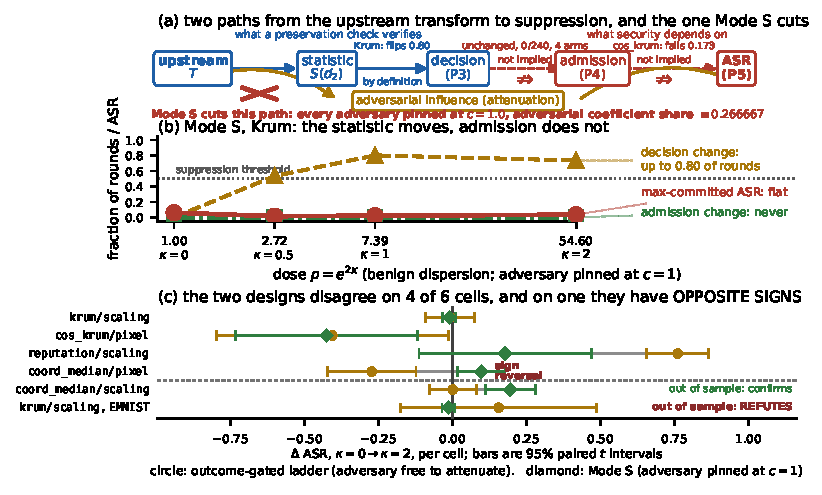
\includegraphics[width=\linewidth]{figures/modeS_causal.pdf}
\caption{\textbf{The paper in one figure: the statistic moves, admission does not, suppression does not follow.} \textbf{(a)} Two paths run from an upstream rescaling $T$ to suppression: the \emph{chain} a preservation criterion reasons along, and a \emph{confounded} path on which $T$ merely attenuates whichever client carries the poison (Lem.~\ref{lem:annihilation}) and reaches ASR \textbf{without passing through $d_2$'s statistic at all}. \textbf{Mode~S cuts the second by construction}, pinning every adversary at $c{=}1$ (\textbf{the one channel the dose closes, and not the only thing it moves}). The admission count pools the four aggregators of \S\ref{sec:targeted_rest}; Krum admits no adversary at any rung, so its zero is a floor (App.~\ref{app:channel_table}). \textbf{(b)} Mode~S, Krum under model-scaling (\S\ref{sec:targeted}): as $\rho$ grows to $54.6$ the \emph{decision} flips in up to $80\%$ of rounds while the \emph{support} of the admitted adversarial mass does not, and max-committed ASR stays inside the pre-specified $\pm0.15$ equivalence margin ($|\Delta|{=}0.026$). Error bars \emph{in this panel} are Student-$t$ $95\%$ intervals on the levels ($n{=}5$). \textbf{(c)} \textbf{Six cells, one contrast each, estimated two ways} (circle: outcome-gated ladder; diamond: Mode~S, adversary pinned at $c{=}1$). \textbf{The designs disagree on $4$ of $6$ cells, and on \texttt{coord\_median}/pixel they have opposite signs}: $\Delta$ASR${=}{-}0.272$ (paired $95\%$ $t$ interval $[-0.422,-0.122]$) against $+0.098$ ($[+0.018,+0.178]$), intervals excluding zero and not overlapping, so \textbf{closing the attenuation channel does not shrink the effect, it reverses its sign}. Above the dashed rule are the four cells a pre-registered mechanism was read off (\emph{training data, not evidence for it}); below are its two out-of-sample cells, one of which \textbf{refutes it, so we withdraw it}.}
\label{fig:modeS}
\end{figure}

\section{Introduction}
\label{sec:intro}

Federated learning~\citep{mcmahan2017communication} is vulnerable to data poisoning~\citep{chen2017targeted,bagdasaryan2020backdoor}, and an arms race has produced defenses~\citep{fung2020foolsgold,pillutla2022robust,yin2018byzantine,blanchard2017machine} with accuracy/robustness trade-offs and none universally dominant (Appendix~\ref{app:related}). \emph{Can we compose them for stronger robustness?} Composition does not even commute: FoolsGold$\to$CoordMedian suppresses a pixel backdoor to ASR $0.076$ while the reverse order reaches $0.732$: a rank aggregator emits one vector rather than per-client updates, so it cannot be an \emph{upstream} stage and the pair collapses to FoolsGold alone, bit-identically. Naive layering fails this way whenever upstream processing destroys what the downstream defense reads.

\textbf{Why the question is sharper without a trusted coordinator.} Such stacks compose independently developed mechanisms among heterogeneous, partially trusted, often pseudonymous participants, so preservation is the obvious discipline to demand of them. Concretely: a contributor clips its own update, a scheduler reweights contributors by reputation, and whoever merges runs a robust aggregator: three parties, three mechanisms, nobody owning the stack. The only check at each seam is that the next stage still reads what it expects, so a preserved statistic is read as evidence the stack is robust. \textbf{That inference is what this paper refutes.} \textbf{The identification problem we isolate is defined independently of model scale}, so we study it in a controlled federated setting and claim no transfer beyond it.

\noindent\textbf{Contributions.} We propose no new defense, and \textbf{our central contribution is a negative identification result}: an outcome-gated comparison of defense pairs cannot determine whether preserving a downstream defense's mechanism is what keeps the composition secure. \emph{Attack-suppression preservation} names the object throughout: suppression of the committed attack surviving composition, instantiated as ASR, never the statistic or the decision that follows; Fig.~\ref{fig:modeS} is the paper in one picture. \textbf{The boundary.} Outcome-gated cross-defense screening is structurally unidentified: its eligibility gate is defined on the same outcome it predicts, so no cross-defense contrast \emph{satisfying this outcome-gated design} identifies the mechanism's contribution and the admissible designs are within-defense (\S\ref{sec:testability}). \textbf{The demonstration.} Statistic preservation is accordingly not a valid causal proxy for attack-suppression preservation, established by intervention rather than correlation: on the identical cell the outcome-gated design estimates $-0.272$ where the intervention estimates $+0.098$, reversing the direction and not merely the precision (\S\ref{sec:targeted}). \textbf{The consequence.} The screening rule follows from the boundary and is nothing more: evaluation prioritization, measurably broken under heterogeneity (App.~\ref{app:prioritization}). \textbf{Also.} The preservation hierarchy (Def.~\ref{def:levels}); mechanism preservation as invariance under positive per-client rescalings (Prop.~\ref{prop:invariance}), with margins on the weighting$\to$aggregator class (Thm.~\ref{thm:bounded_reweight}), supporting machinery, safe at \emph{both} extremes of the weight ratio, so dispersion alone mispredicts; counterexamples across four aggregators of three structural kinds; and the negative replicated in a second invariance class and on a second dataset and architecture, while refuting the cross-arm admission ordering we had predicted. Scope is inventoried once, in Tables~\ref{tab:scope_levels} and~\ref{tab:tiers}: what each claim does \emph{not} license, and the evidence tiers (App.~\ref{app:contributions}).

\section{What Preservation Could Mean: A Hierarchy of Five Levels}
\label{sec:framework}

\emph{What does it mean for a composition to preserve a defense?} Every per-client defense we consider acts as a positive scalar rescaling $T(u_i) = c_i u_i$, which gives the invariance question a sharp \emph{algebraic} answer (Prop.~\ref{prop:invariance}), but writing C2 as an invariance of the statistic $S$ leaves a gap our own experiments exposed. Three different things can be preserved: what the downstream defense \emph{reads} (P1--P2), what it \emph{decides} and what \emph{survives} it (P3--P4), and whether the attack is still \emph{suppressed} (P5). They come apart, so we name the levels and ask of each whether it determines the one below:

\begin{center}\small\vspace{-7pt}\setlength{\tabcolsep}{5pt}
\begin{tabular}{@{}lll@{}}
\toprule
Level & What is preserved & Determines the level below? \\
\midrule
(P1) & the statistic's value & yes, by definition \\
(P2) & the ordering it induces & yes, by definition \\
(P3) & the decision $d_2$ makes & \textbf{no}, by counterexample (\S\ref{sec:targeted}) \\
(P4) & the adversarial contribution admitted & \textbf{no}, by counterexample (\S\ref{sec:targeted_rest}) \\
(P5) & suppression of the committed attack & --- \\
\bottomrule
\end{tabular}
\vspace{-5pt}\end{center}

\noindent \textbf{Both breaks are measured}, at fixed $d_2$ and attack: Krum's decision flips in up to $80\%$ of rounds with the adversarial mass it admits unchanged (\S\ref{sec:targeted}), and \texttt{cos\_krum}'s decision and admitted mass are bit-identical while ASR falls $0.173$ (\S\ref{sec:targeted_rest}); Fig.~\ref{fig:story} draws the chain and both breaks.

The algebra fixes which level a given composition sits at: cosine similarity is exactly invariant, so C2 holds for every $\cdot \to$ FoolsGold composition; coordinate ordering survives only under a bounded-ratio condition; consensus distance and residual magnitude are not invariant at all, so $\cdot \to$ Reputation compositions are C2 failures; norm clipping does not blind FoolsGold, though it does blind Reputation.

\begin{definition}[Preservation levels]
\label{def:levels}
For an upstream transform $T$ and a downstream defense $d_2$ reading statistic $S$:
\begin{enumerate}[noitemsep,topsep=2pt,label=(P\arabic*)]
\item \textbf{Value invariance:} $S(T(U)) = S(U)$.
\item \textbf{Ordering invariance:} $S(T(U)) = \varphi(S(U))$ for some $\varphi$ preserving the ordering $S$ induces on clients. \emph{(this is C2)}.
\item \textbf{Decision invariance:} the client or coordinate $d_2$ actually selects is unchanged.
\item \textbf{Adversarial contribution (admission) invariance:} the adversarial input $d_2$ admits into its aggregate is unchanged. \emph{Admission} is the pre-registered term throughout for how much adversarial input survives $d_2$: a level, not one measurable quantity, instantiated by whatever each rule exposes: Krum's and \texttt{cos\_krum}'s selected-client indicator, \texttt{coord\_median}'s selected-coordinate share, reputation's adversarial weight share, which is why App.~\ref{app:channel_table}'s influence column is aggregator-specific.
\item \textbf{Attack-suppression preservation:} ASR stays below threshold.
\end{enumerate}
We target (P4)$\not\Rightarrow$(P3) in \S\ref{sec:targeted} and (P4)$\not\Rightarrow$(P5) in \S\ref{sec:targeted_rest}. The conditions (C0)--(C3) the levels induce (\textbf{the rule being C1$\wedge$C2}) are in App.~\ref{app:framework} and~\ref{app:conditions}.
\end{definition}

\paragraph{What the theory delivers: supporting machinery, not the claim.} For a per-client \emph{weighting} into a \emph{rank-based} or \emph{geometric} aggregator, Thm.~\ref{thm:bounded_reweight} gives sufficient conditions for $d_2$'s ordering to survive: it \textbf{certifies mechanism preservation, not security} and bounds no ASR. Its one prediction, admitted adversarial mass $\Lambda_a \leq 12.6\%$ against a realized $\leq 1.8\%$, goes vacuous as the separation margin approaches $1$, which heterogeneity reaches, and does not follow from a $(d_1,d_2)$ definition pair alone, as a screen would need (App.~\ref{app:proofs}).

\section{The Testability Boundary}
\label{sec:testability}

\emph{Why can we not simply compare many defense pairs?} The natural test keeps pairs whose constituents already suppress the attack and asks whether the composition preserves it. That is exactly where identification is lost. \textbf{The boundary in words} (Prop.~\ref{prop:identification}, formal in App.~\ref{app:boundary}): let a screen certify $(d_1 \to d_2)$ only if an \emph{eligibility gate} holds: some constituent already suppresses the attack, measured by the same outcome metric and threshold the screen predicts for the composition, and a mechanism condition $P$ holds, fixed by the two defenses' definitions alone. Four cells follow, and that design never fills two of them:

\begin{center}\small\vspace{-7pt}\setlength{\tabcolsep}{5pt}
\begin{tabular}{@{}lll@{}}
\toprule
Mechanism condition & $d_2$ suppresses $a$ alone & it does not \\
\midrule
$P$ holds (preserved) & observed: every certified pair & \textbf{empty by the gate} \\
$\neg P$ (destroyed) & observed: predicted-FAIL pairs & \textbf{empty by the gate} \\
\bottomrule
\end{tabular}
\vspace{-5pt}\end{center}

\noindent Reading down a column is the contrast that would identify $P$'s contribution, and \textbf{the only column in which $d_2$ is not already doing the work is empty}, for every menu a screen of this form could range over: excluded by design, not undersampled: more data cannot fill a cell the design never permits. The gate cannot be dropped either, because without it C1 is vacuous. So wherever our conditions certify a pair, a low composition ASR is attributable to $d_2$'s standalone strength rather than to preservation. Equivalently, this is selection on a collider~\citep{elwert2014endogenous,pearl2009causality}: the gate is a descendant of both $P$ and $d_2$'s standalone effectiveness, so conditioning on it makes them co-vary. The hazard is standard; the gate reading as hygiene rather than as the step that removes identification is not, and we made that mistake ourselves (\S\ref{sec:dose_response}).

\paragraph{The admissible design, derived: the practical contribution.} Read forwards the boundary is \emph{constructive}, each clause forced by a term in Prop.~\ref{prop:identification}: (1) hold $d_2$ and the attack fixed, so the gate's input is the same quantity on both sides of every contrast; (2) intervene on the upstream transform rather than selecting a different $d_2$, whose variation is what empties the cell; (3) pin the adversarial coefficient channel, since an upstream that attenuates the adversary moves the outcome by a route unrelated to $d_2$'s statistic, the confound that inverted our own sign; (4) measure every channel: aggregate displacement, decision, admission, influence. \S\ref{sec:targeted} is clause (3) as an instrument; the six-step form is in App.~\ref{app:conclusion}. A second boundary bounds what such a screen can \emph{find}: \textbf{no \emph{emergent} composition can satisfy an inherited-suppression gate}, our own lowest-ASR composition being the witness: FG$\to$RFA reaches $0.093$ where FoolsGold alone reaches $0.732$, so at $|\mathcal{E}|/|\mathcal{S}|{=}1/5$ the bound caps recall at $80\%$, above the $40\%$ we measure (App.~\ref{app:prioritization}).
\label{sec:prioritization}

\section{Statistic Preservation Does Not Identify Attack-Suppression Preservation}
\label{sec:targeted}

\emph{Does disturbing what a defense reads actually cost suppression?} The claim: it need not, and \textbf{the design that says otherwise gets the sign backwards}. Our pre-registered pooled hypothesis (H1), that ASR rises with disturbance of the statistic $d_2$ reads, is rejected, the effect \emph{negative}: that ladder moved adversarial influence and the statistic together (\S\ref{sec:dose_response}). We adjudicate C2's implication that losing (P3) means losing (P5) by oracle intervention on two arms in two invariance classes, not by a general law.

\paragraph{The instrument, as a counterfactual.} The clean question asks what happens when the downstream statistic changes but the adversary cannot become weaker. \textbf{Mode S} enforces exactly that: it pins every adversary's coefficient at $c{=}1.0$ and spreads only the benign clients over $\rho = e^{2\kappa}$, holding the adversarial coefficient share constant at $0.266667$ to within float32 read-back noise, closing Figure~\ref{fig:modeS}(a)'s attenuation path, so a rise in ASR here cannot be attenuation. Mode~S and Mode~A (\S\ref{sec:validation}) are causal instruments built from adversary identity: they measure mechanism-level effects rather than emulate deployable defenses (Table~\ref{tab:scope_levels}, App.~\ref{app:targeted_full}).

\paragraph{Two readings of C2, frozen against each other.} \emph{The statistic reading}: what matters is disturbance of $d_2$'s statistic, read off its \emph{decisions}. \emph{The admission reading}: what matters is the \emph{adversarial input $d_2$ admits}. Mode~S disturbs Krum's selection heavily while leaving the mass it admits untouched, so that arm adjudicates (Table~\ref{tab:targeted}, the pre-registration's H-statistic and H-admission): as $\rho$ climbs to $54.6$ we find the decision changing in up to $0.80$ of rounds while the adversarial mass admitted changes in none of them, and ASR showing no evidence of the predicted increase, remaining inside the pre-specified equivalence margin ($p_{\uparrow}{=}0.70$, $|\Delta|{=}0.026<0.15$). \textbf{The statistic reading is refuted}: statistic and decision disturbance need not change suppression once the adversarial coefficient share is held fixed. \emph{On this arm the zero is a floor}: Krum admits no adversary at any rung, so the dissociation is read across all four aggregators, each under its own committed attack:

\begin{center}\small\vspace{-7pt}\setlength{\tabcolsep}{5pt}
\begin{tabular}{@{}llrrrr@{}}
\toprule
Aggregator & Kind & $\Delta$ dec. & $\Delta$ adm. & $\Delta \Lambda_a$ & $\Delta$ ASR \\
\midrule
Krum & selector & 0.733 & 0.000 & 0.000 & $-0.026$ \\
Reputation & weighted averager & 1.000 & 0.000 & 0.020 & $+0.178$ \\
Cosine-Krum & cosine-invariant selector & 0.000 & 0.000 & 0.000 & $-0.425$ \\
Coord.\ median & coordinate order statistic & 0.482 & 0.000 & 0.033 & $+0.098$ \\
\bottomrule
\end{tabular}
\vspace{-5pt}\end{center}

\noindent $\Delta$~adm.\ is the \emph{support} of the admitted adversarial mass: it never moves in any of the $60$ measured rounds of any arm, including the $48$ per arm where reputation and \texttt{coord\_median} carry adversarial mass at baseline. $\Delta\Lambda_a$ is the separate question of how much weight the adversary's direction carries. \texttt{cos\_krum}'s $-0.425$ is the full-ladder endpoint, below our accuracy floor; the witness we rest on is its first, gate-passing rung ($0.173$, \S\ref{sec:targeted_rest}); App.~\ref{app:channel_table} adds EMNIST-byclass and the score-only control.

\paragraph{What the instrument does not hold fixed, and the pre-registered control that closes it.} Mode~S does not identify the effect of statistic disturbance in isolation: it identifies the effect of the upstream intervention while holding the adversarial coefficient share fixed, which is what lets statistic and decision disturbance be \emph{dissociated} from suppression rather than shown to be inert. Mode~S pins the \emph{adversarial} coefficients and nothing else: the dose also moves Krum's pairwise distances, \emph{which} benign client it selects, and the \textbf{magnitude and geometry of the update actually aggregated}. That third channel is measured: App.~\ref{app:channel_table}'s $\Delta$~agg.\ column, the aggregate the defense \emph{emits}, reads $\mathbf{0.892}$ here (App.~\ref{app:decomposition}). \textbf{Score-only Krum} closes it: Krum scores the transformed stack and so makes the same selection, but the \emph{untransformed} selected update is aggregated: the decision channel preserved, the magnitude and geometry change removed. Rules were frozen at \texttt{35788d9} before any score-only ASR existed, $\Delta > +0.15$ meaning the published result was partly a magnitude artifact. We find $\Delta = -0.023$ ($0.062 \to 0.039$) against $-0.026$ uncontrolled on the identical cell, at the same $\Delta$~dec.\ of $0.733$, the refuting threshold $0.212$ nowhere approached and every rung clearing the accuracy floor, so the central claim is instrumented against two independent confounds, attenuation and magnitude (App.~\ref{app:score_only}).

\paragraph{A pre-registered replication that refutes the positive half, and the sign reversal.} \texttt{coord\_median} under the pixel backdoor is \emph{rank-discordant}: of the interpretable arms it has the smallest decision change ($0.482$) and the largest admission-level change ($\Delta\Lambda_a{=}0.033$), so the two readings predict opposite rank positions for its rise, and thresholds were frozen against the two published rises (confirm if $\Delta>+0.178$, refute if $\Delta<+0.150$). We find $\Delta=+0.098$, which \textbf{refutes the admission \emph{ordering}}: the arm with the largest admission-level change rose \emph{less} than one with a smaller change. The decision reading does not predict it either ($R^2{=}0.239$ pooled). What replicates is the negative on a coordinate-wise order statistic: a decision change of $0.482$ costs no suppression by the frozen margin, at accuracy $0.698$. Identity ASR here is $0.443$, so equivalence is to the \emph{identity rung}; the rise is positive in $5/5$ seeds (post-hoc): small and consistent, not zero.

\paragraph{The confounded design gets the causal sign wrong.} On this identical cell (matched displacement, decision change and clean accuracy, Table~\ref{tab:comparability}), closing one channel reverses the sign:

\begin{center}\small\vspace{-7pt}\setlength{\tabcolsep}{6pt}
\begin{tabular}{@{}llr@{}}
\toprule
Design & The adversarial coefficient & $\Delta$ ASR \\
\midrule
Outcome-gated ladder (\S\ref{sec:dose_response}) & free to attenuate & $-0.272$ ($p_{\downarrow}{=}0.0015$) \\
Mode~S intervention (\S\ref{sec:targeted}) & pinned at $c{=}1$ & $+0.098$ \\
\bottomrule
\end{tabular}
\vspace{-5pt}\end{center}

\noindent \textbf{The confounded design does not lose power, it gets the sign wrong.} Closing the attenuation channel inverts the effect rather than sharpening it: a criterion calibrated against the confounded contrast would have been calibrated against the confound, so \S\ref{sec:testability}'s boundary is not a technicality about power. \textbf{Downstream-statistic preservation is not, in general, sufficient to establish attack-suppression preservation} (Prop.~\ref{prop:nonidentifiability}): no predicate of the statistic alone determines the admitted adversarial mass, and none of that mass alone determines suppression: the title claim, by counterexample \emph{within this class} (Table~\ref{tab:scope_levels}).

\section{What the Boundary Licenses, and What We Found}
\label{sec:validation}
\label{sec:prospective}
\label{sec:metric_swap}

We validate on CIFAR-10 with a 4-layer CNN, $N{=}10$ clients, $f{=}0.2$ adversarial, two committed attacks (model-scaling, pixel backdoor), at $n{=}5$ seeds per cell; \emph{ASR} means \emph{max-committed ASR}; the rest is fixed in App.~\ref{app:details}. The core evidence is a seed-matched intervention on one cell, not a mean comparison across cells.

\paragraph{The confounded ladder that motivated the instrument, and the sign it got wrong.}
\label{sec:dose_response}
Our earlier suites tried to validate C2 by \emph{choosing a different downstream defense}, the move Prop.~\ref{prop:identification} rules out. Varying only the \emph{dose} at fixed $d_2$ and attack ($\kappa{=}0$ bit-identical to $d_2$ standalone) refutes that suite's pooled prediction that disturbance predicts each arm's rise: $\rho_s{=}{+}0.351$, one-sided $p{=}0.091$ against a frozen $p<0.05$, and in three of four arms ASR \emph{falls} as the dose rises ($80$ runs, one arm confirming decisively; Table~\ref{tab:dose_outcome}). \textbf{The fault is ours and is measured}: at fixed $\mathrm{mean}(c)$ a large spread mostly \emph{dilutes} whichever client carries the poison, so this is attenuation, not statistic disturbance (App.~\ref{app:dose_caveats}, \ref{app:delta_c}).

\paragraph{The dissociation holds across four aggregators and replicates on a second dataset.}
\label{sec:targeted_rest}
Applying the instrument to that ladder, most of the one confirmation was attenuation: with the adversary's share pinned, reputation's rise at $\rho{=}54.6$ shrinks from $+0.762$ to $+0.178$, and what remains tracks a small \emph{admission} change, not the large decision change (App.~\ref{app:targeted_full}). The class-(a) control refutes us the other way: \texttt{cos\_krum}'s selection is bit-identical at every rung yet ASR is $0.584$ at the identity (it never suppresses) and \emph{falls} $0.173$ at the first accuracy-gate-passing rung (one-sided $p{=}0.044$, $5/8$ seeds); the full-ladder fall sits below our accuracy floor, so \textbf{the gate-passing rung is the witness}. \textbf{Mode A} (payload share at fixed dispersion) separates Thm.~\ref{thm:bounded_reweight}'s two regimes: confirmed for \texttt{coord\_median}, refuted for reputation. A \emph{pre-registered} replication on EMNIST-byclass/\texttt{simple\_cnn} moves the decision on $0.643$--$0.714$ of rounds with the adversary never admitted and suppression inside the frozen $\pm0.15$ margin ($\Delta=-0.017$ beside CIFAR-10's $-0.026$): \textbf{replicated} on a second dataset and architecture, never ``generalizes'' (App.~\ref{app:channel_table}, \ref{app:validation_full}).

\paragraph{And what a screen then buys.} Only the $13/20$ prospective sub-tier risks falsification, limited by our menu: FLTrust suppresses both attacks alone ($0.048$), so its pairs are out of scope or near-identities, and two further attempts to validate the \emph{screen} were defeated by the same confound. \textbf{A third closed a census.} The region Prop.~\ref{prop:invariance}(a) settles \emph{exactly} is $3\times3$; its $2$ unspent cells and $2$ measured-C2-fail controls were labelled at \texttt{96f8856}, and \textbf{all four landed as registered}. It holds \textbf{one} low-ASR pair, rep$\to$\texttt{cos\_krum} at $0.263$, which neither constituent suppresses alone, \textbf{and the criterion selects it}: C2 alone admits $9$ ($11\%$, $90$ runs), C1$\wedge$C2 admits $1$ ($100\%$/$100\%$, $10$). \textbf{Where invariance is exact the trade reverses}, on one accuracy-gated cell at $n{=}3$ whose C1 input is itself seed-count-contingent ($33\%$ ungated; App.~\ref{app:census}). \textbf{Scale:} the PASS predictions hold at $N{=}100$/ResNet18, far from converged accuracy. Under \emph{one} adaptive stress test FG$\to$RFA rises $3.7\times$: \textbf{inherited robustness is not adaptive robustness} (App.~\ref{app:validation_full},~\ref{app:secondary},~\ref{app:confusion}).

\section{Conclusion}
\label{sec:conclusion}

\textbf{The finding.} Downstream-statistic preservation is not sufficient to identify preserved attack suppression. An intervention changes a defense's statistic and decision substantially without changing the adversarial mass it admits or the suppression that follows; conversely a bit-identical statistic and decision coexist with a change in suppression, each direction with a measured witness.

\textbf{Why.} An outcome-gated cross-defense comparison conditions on the same outcome it seeks to explain, so it cannot separate mechanism preservation from standalone effectiveness: a structural identification boundary (Prop.~\ref{prop:identification}) no amount of additional data within that design removes. Within-defense intervention fixes $d_2$ and the attack instead: on the identical cell \textbf{the confounded design does not lose power, it gets the sign wrong}.

\textbf{The implication.} Evaluate composed defenses by measuring the adversarial contribution that survives the downstream mechanism, not by inferring security from the statistic it consumes. That object is (P4), which Mode~S reads only by knowing adversary identity, so we identify the channel rather than screen for it (App.~\ref{app:conclusion}). The open question: \textbf{can (P4) be estimated without knowing who is malicious?}


\bibliographystyle{abbrvnat}
\bibliography{references}

\appendix
\clearpage

\noindent Table~\ref{tab:scope_levels} sits ahead of the appendices because it governs all of them: it is the one place each scope condition is stated, and no later section restates them at each use.

\begin{table}[h]
\centering\scriptsize\setlength{\tabcolsep}{4pt}
\caption{\textbf{Scope of claims.} The one place each scope condition is stated. \textbf{Claims do not transfer upward}: the formal guarantee does not certify the general framing, and the empirical figures certify neither level above them.}
\label{tab:scope_levels}
\begin{tabular}{@{}p{0.095\linewidth}p{0.285\linewidth}p{0.545\linewidth}@{}}
\toprule
\textbf{kind} & \textbf{content} & \textbf{status, and what it does \emph{not} license} \\
\midrule
\textbf{General} & An evaluation gated on the outcome it predicts cannot identify the mechanism's contribution; admissible designs are within-defense (Prop.~\ref{prop:identification}, Prop.~\ref{prop:emergent}). & \textbf{Proved, and not specific} to FL, to backdoors, or to our conditions. Licenses no claim that a composition \emph{is} secure, nor that mechanism preservation implies suppression. \\
\addlinespace
\textbf{Formal} & Mechanism preservation as \emph{invariance} under \textbf{positive per-client rescalings} $T(u_i)=c_iu_i$, $c_i>0$, into specific rank and geometric aggregators (Thm.~\ref{thm:bounded_reweight}, Lem.~\ref{lem:annihilation}, Cor.~\ref{cor:aggregate_mass}). & \textbf{Proved on that class only}: a \emph{laboratory} for composition, not a model of FL defenses in general. A $d_1$ that alters participation, carries cross-round state, mixes clients, or aggregates first has no such $T$ and is \textbf{covered by nothing here} (C0, applied retrospectively to arms frozen before it). \textbf{Bounds no ASR}, and Regime~A's condition is not operationally checkable ($S$ is not a stable per-attack constant). \\
\addlinespace
\textbf{Empirical} & \S\ref{sec:targeted}'s interventions and \S\ref{sec:validation}'s 42-pair menu: CIFAR-10, CifarCNN/ResNet18, $N\in\{10,100\}$, $f\in[0.05,0.6]$, Dirichlet $\alpha{=}0.5$, \textbf{star topology}, three attack families; one arm on EMNIST-byclass/\texttt{simple\_cnn}. & \textbf{Measured} at $n{=}5$ seeds per cell ($n{=}8$ for \texttt{cos\_krum}, $n{=}3$ on EMNIST-byclass), fixed before the runs, so intervals are wide and \textbf{no null is read as flatness} without a pre-registered equivalence margin. Dataset transfer is tested on the flagship arm alone: ``replicated on a second dataset and architecture,'' never ``generalizes''. \textbf{For the \emph{screen}, dataset transfer on EMNIST-byclass is out of scope rather than merely untested: no single defense measured there suppresses the committed pixel backdoor alone (minimum $0.609$), so C1's per-attack precondition fails over the menu measured} (\S\ref{app:femnist_c1}). \textbf{``Refuted''} always means a pre-registered \emph{directional} hypothesis was rejected against a rule frozen for it, \textbf{never} that a mathematical claim was disproved. \\
\addlinespace
\textbf{Both instruments are oracles} & Mode~S and Mode~A build $c_i$ from adversary identity, as does $\Delta_c$. & They \textbf{identify a causal channel and are not screens}; computing (P4) without adversary identity is our open problem, and admission is \emph{a direction to measure}, not a validated predictor. C1 and all built on it assume a \textbf{committed} adversary: what is bounded is \emph{inherited} robustness under a fixed attack, \textbf{never adaptive robustness}. \\
\bottomrule
\end{tabular}
\end{table}

\section{The composition model and the invariance classification}
\label{app:framework}

\paragraph{The two witnesses under Definition~\ref{def:levels}, and which rung each rests on.} \textbf{(P1)$\Rightarrow$(P2)$\Rightarrow$(P3) hold by definition}: \textbf{logical implications, not empirical claims}; their content is that they stop at (P3), and \S\ref{sec:framework}'s table states both breaks below it. \emph{Holding} decision \emph{and} admission invariance does not deliver suppression: \texttt{cos\_krum} falls $0.173$ by the first rung alone through the magnitude channel, at $\rho{=}2.72$, where clean accuracy moves only $0.599 \to 0.567$ and our accuracy gate passes (Appendix~\ref{app:dose_detail}). Across the whole ladder it falls $0.425$, but that endpoint sits below our accuracy floor, so \textbf{the gate-passing rung is the witness we rest on} (\S\ref{sec:targeted_rest}). \emph{Losing} decision invariance does not cost suppression: Krum's selection flips in up to $80\%$ of rounds under an intervention pinning the adversarial mass, and its ASR stays inside the pre-specified equivalence margin ($|\Delta|{=}0.026 < 0.15$) (\S\ref{sec:targeted}). So a criterion stated at (P1)--(P2) constrains security in \emph{neither} direction, \textbf{(P4), where the security content sits, is not sufficient for (P5)} either, and \textbf{the hierarchy answers ``which level does a security claim have to be stated at?'', not ``which level predicts ASR?''}

\begin{definition}[Defense composition]
\label{def:composition}
Given defenses $d_1$ and $d_2$, composition $(d_1 \to d_2)$ operates as: $d_1$ produces per-client transformed updates $U' = \{T_{d_1}(u_i)\}_{i=1}^K$; $d_2$ aggregates $U'$ using its standard algorithm. For FoolsGold$\to$CoordMedian, FG outputs $\{w_i u_i\}$ and CoordMedian takes the \emph{unweighted} coordinate-wise median of the $K$ transformed values, not a ``weighted median''. Clients with $w_i = 0$ are \textbf{not removed} but reach $d_2$ as zero vectors, so at least one point of $U'$ is always the origin, which is what Lemma~\ref{lem:annihilation} is about.
\end{definition}

Each defense suppresses malicious updates through a \emph{discriminative property} (a structural feature separating adversarial from benign contributions) and the property is defense-class-specific: \emph{similarity spread} (FoolsGold), \emph{coordinate ordering} (TrimmedMean, CoordMedian), \emph{residual magnitude} (RFA), \emph{consensus distance} (Reputation, in $\ell_2$ from the coordinate-wise median) and \emph{norm magnitude} (NormClip). Mechanism preservation is then governed by whether $d_1$'s transform leaves $d_2$'s property intact, and because every per-client defense we consider acts as a positive scalar rescaling, that question has a sharp answer:

\begin{proposition}[Invariance classes under positive per-client rescaling]
\label{prop:invariance}
Let $T(u_i) = c_i u_i$ with $c_i > 0$, \textbf{strictly}: the form taken by NormClip ($c_i = \min(1, \tau/\|u_i\|)$), Reputation ($c_i \propto e^{-d_i/s}$) and RFA-reweighting ($c_i \propto 1/\max(\|u_i - \mu'\|, \varepsilon)$), each positive by construction. \textbf{FoolsGold is deliberately not in that list}: its shift-and-clamp gives the least-trusted client weight exactly $0$ in \emph{every} round (2 of 5 clients here), so FoolsGold-as-$d_1$ falls outside the hypothesis and is governed by Lemma~\ref{lem:annihilation} rather than by (a)--(c). Then:
\begin{enumerate}[noitemsep,topsep=2pt,label=(\alph*)]
\item \textbf{Cosine similarity is exactly invariant:} $\cos(c_i u_i, c_j u_j) = \cos(u_i, u_j)$. Hence FoolsGold's weight vector is unchanged, $w(T(U)) = w(U)$, and \textbf{C2 holds for every $\cdot \to$ FoolsGold composition}.
\item \textbf{Coordinate ordering is not invariant} in general; it survives under the bounded-ratio condition of Theorem~\ref{thm:bounded_reweight}(1).
\item \textbf{Consensus distance and residual magnitude are not invariant:} heterogeneous $c_i$ can invert their ordering, so $\cdot \to$ Reputation compositions are C2 failures and $\cdot \to$ RFA requires the separation condition of Theorem~\ref{thm:bounded_reweight}(2).
\end{enumerate}
\end{proposition}

\noindent So mechanism preservation is a question about the \emph{invariance class} of the downstream signal, and the classification corrects a natural but wrong intuition: norm clipping does not blind FoolsGold, though it does blind Reputation, whose signal is consensus distance rather than similarity.

\paragraph{The framework in general form.} The structure does not depend on rescaling. Write $d_2$'s discriminative property as a statistic $S(U)$ and let $T$ be $d_1$'s per-client transform; then $(d_1 \to d_2)$ is \textbf{mechanism-preserving} when $S(T(U)) = \varphi(S(U))$ for some $\varphi$ preserving the ordering $d_2$ acts on. C2 is exactly that requirement, C3 asks in addition that $\varphi$ not compress the gap below $d_2$'s operating threshold, and Proposition~\ref{prop:invariance} is the case $T(u_i)=c_iu_i$ (Appendix~\ref{app:proofs}), so the conditions are algebraic rather than experimental. It also states the real limit: \textbf{a $d_1$ whose transform is not per-client} (mixing updates, or carrying cross-round state) \textbf{has no $T$ of this form, and nothing here applies}.

\noindent \textbf{The full causal chain.} Definition~\ref{def:levels} is a prefix of a longer one: statistic $\to$ \emph{decision} $\to$ \emph{admission} $\to$ \emph{aggregate adversarial influence} $\to$ per-round update $\to$ persistence $\to$ \emph{ASR}. \textbf{We measure the four emphasized links, not update geometry or persistence dynamics}: an acknowledged gap, not an assumed-benign one. A selection flipping from one benign client to another disturbs the statistic maximally and the mechanism not at all, which is why (P3) and (P4) come apart. \textbf{``\emph{Mechanism}'' always means the downstream defense's \emph{discriminative operation}, never its security behaviour}, that implication being what this paper refutes.

\section{The signal-preservation conditions in full}
\label{app:conditions}

\begin{definition}[Signal-Preservation Conditions]
\label{def:conditions}
Composition $(d_1 \to d_2)$ is predicted to suppress attack $a$ when: \textbf{(C0)} $d_2$'s mechanism is load-bearing, $\mathrm{ASR}(d_1,a)\ge 0.5$ for some committed $a$: a condition on the criterion's \emph{domain} that \textbf{never certifies a pair}, and one we formulated only after \S\ref{sec:prospective} made it bind, so it is applied \textbf{retrospectively} and is \textbf{not part of what the 42 pairs validate}; \textbf{(C1)} some constituent suppresses \emph{every} committed attack alone, $\min_{d\in\{d_1,d_2\}}\mathrm{ASR}(d,a) < 0.5$ for all $a$, defined through the same threshold that constitutes the outcome, hence an \textbf{empirical prerequisite and not a mechanistic property}; \textbf{(C2)} $d_1$'s transform does not destroy $d_2$'s discriminative property, decided from definitions alone by Proposition~\ref{prop:invariance}; \textbf{(C3)} it does not compress the quantitative margin below $d_2$'s operating threshold. \textbf{The prioritization rule is C1$\wedge$C2}, C3 demoted to a \emph{margin diagnostic} (Appendix~\ref{app:condition_scoring}); the pre-registered labels of \S\ref{sec:validation} were frozen with C3 in the gate and are \emph{not} relabelled. \textbf{Theorem~\ref{thm:bounded_reweight} bounds no ASR}: that mechanism preservation plus C1 predicts \emph{low} ASR is a \emph{separate} empirical hypothesis, tested in \S\ref{sec:validation}, and \textbf{neither stage alone establishes low ASR, nor does their conjunction} (stage structure, Appendix~\ref{app:conditions}).
\end{definition}

Definition~\ref{def:conditions} in the body states the four conditions and every disclosure attached to them; what follows is the same criterion with its \emph{stage structure}, which is worth separating because conflating the stages is the main source of confusion about what the framework claims.

\noindent
Composition $(d_1 \to d_2)$ suppresses attack $a$ when the conditions below hold. The criterion is a \textbf{two-stage screen}, and we label the stages because conflating them is the main source of confusion about what the framework claims: stage~1 is empirical screening of the \emph{constituents}, stage~2 is mechanistic screening of the \emph{composition}.

\smallskip
\noindent\textbf{Stage 0: applicability} (C0). Whether the framework has anything to say about this pair at all. This is a condition on the criterion's \emph{domain}, and Lemma~\ref{lem:testability} is stated over it together with C1.
\begin{description}[topsep=2pt,parsep=0pt,itemsep=3pt,leftmargin=0pt,labelindent=0pt,itemindent=\labelsep]
\item[(C0) The downstream mechanism is load-bearing.] $\mathrm{ASR}(d_1,a) \geq 0.5$ for at least one committed attack $a$. C2 and C3 concern preservation of \emph{$d_2$'s} mechanism, so they carry information only when that mechanism does work the composition needs: if $d_1$ alone suppresses everything, the composition inherits that suppression and a correct prediction is correct for a reason the framework did not supply. The asymmetry is deliberate: a strong \emph{$d_2$} is the intended case. \textbf{Failing C0 removes a pair from the criterion's domain; it never certifies one.} \emph{Provenance:} C0 was vacuous on the menu the framework was developed on (strongest single defense $0.519$) and was formulated only after the prospective suite of \S\ref{sec:prospective} made it bind, so it is applied \textbf{retrospectively} and is \textbf{not part of what the 42 pairs validate} (Appendix~\ref{app:prospective}).
\end{description}

\smallskip
\noindent\textbf{Stage 1: empirical constituent screening} (C1). Read off standalone evaluations. This screens; it does not explain, and it is not a mechanistic claim.
\begin{description}[topsep=2pt,parsep=0pt,itemsep=3pt,leftmargin=0pt,labelindent=0pt,itemindent=\labelsep]
\item[(C1) Individual effectiveness.] For \emph{every} committed attack $a$ in the evaluated set, $\min_{d \in \{d_1,d_2\}} \mathrm{ASR}(d,a) < 0.5$. The quantifier matters: our headline metric is the \emph{maximum} over attacks, so requiring a suppressing constituent for only one attack would license compositions that fail on the other. C1 is defined through the same ASR threshold that constitutes the outcome, so it is an \textbf{empirical prerequisite, not a mechanistic property}: the one condition that cannot be checked without running something.
\end{description}

\smallskip
\noindent\textbf{Stage 2: mechanistic composition screening} (C2, with C3 as a diagnostic). Determined by $d_1$'s and $d_2$'s definitions alone, no experiment required, and what Theorem~\ref{thm:bounded_reweight} proves. \textbf{The evaluation-prioritization criterion is C1$\wedge$C2}, with C3 retained as a \textbf{margin diagnostic} rather than a gate for the reasons scored in Appendix~\ref{app:condition_scoring}. \emph{The pre-registered labels of \S\ref{sec:validation} were frozen with C3 in the gate and are not relabelled}, and the demotion changes no reported number.
\begin{description}[topsep=2pt,parsep=0pt,itemsep=3pt,leftmargin=0pt,labelindent=0pt,itemindent=\labelsep]
\item[(C2) Discriminative-property preservation.] $d_1$'s transform does not destroy $d_2$'s discriminative property, as determined by Proposition~\ref{prop:invariance}: automatic for cosine-similarity downstream defenses, conditional for coordinate ordering, and violated for consensus distance under heterogeneous rescaling.
\item[(C3) Margin preservation.] $d_1$ does not compress the quantitative margin below $d_2$'s operating threshold. For rank aggregators: extremeness gap survives reweighting. For geometric aggregators: separation condition holds on transformed points.
\end{description}
\textbf{What is proved and what is hypothesised.} Stage~1 is empirical and outcome-defined, stage~2 mechanistic, and \textbf{neither alone establishes low ASR, nor does their conjunction}: Theorem~\ref{thm:bounded_reweight} establishes that C2$\wedge$C3 preserve $d_2$'s discriminative mechanism on the reweighted inputs and \textbf{bounds no ASR}. That mechanism preservation plus C1 predicts \emph{low ASR} is a separate empirical hypothesis, tested in \S\ref{sec:validation}.

\section{The four channels, all four aggregators}
\label{app:channel_table}

\noindent Endpoint change ($\kappa{=}0$ against $\kappa{=}2$) in each measured channel under Mode~S, for every downstream defense in the paper. \textbf{The first column, $\Delta$~agg., is the relative displacement of the aggregate the defense \emph{emits}}, $\|\mathrm{agg}(T(U)) - \mathrm{agg}(U)\|/\|\mathrm{agg}(U)\|$: what enters training, and \textbf{not} the value of a scoring statistic. The measured channels are therefore aggregate displacement, decision, admission and influence. \textbf{Recomputed, not transcribed}: every cell is emitted by \texttt{experiments/build\_channel\_table.py} from \texttt{admission\_} \texttt{measurement.json}, \texttt{femnist\_admission.json}, \texttt{targeted\_dose/summary.json}, \texttt{dose\_} \texttt{replication/summary.json} and \texttt{dose\_femnist/summary.json} under \texttt{results/}, which the script only reads; it also asserts that the identity rung displaces nothing ($0.00\mathrm{e}{+}00$ for all six rows). \textbf{The sixth row is the score-only control} (Appendix~\ref{app:score_only}): the first row's arm with the magnitude channel closed, so its aggregate column is the re-selection component alone (from \texttt{displacement\_decomposition.json}) and its decision, admission and influence columns are the first row's own numbers, score-only leaving the selection untouched; its ASR comes from \texttt{score\_only/summary.json}, which the emitter refuses to merge into the ASR sources it shares cell keys with, so it cannot shadow the first row's published number. The influence column is \textbf{aggregator-specific by necessity} (a selector has no weights) and its instantiation is: adversarial share of the Weiszfeld/reputation weight mass for the averager, adversarial share of selected coordinates for the order statistic, and the indicator that an adversarial update is selected at all for the two selectors. Earlier drafts labelled this arm ``FEMNIST'' in the tables while the prose said EMNIST-byclass: the loader reads torchvision \texttt{EMNIST(split="byclass")} under a \texttt{femnist} key and partitions it by the label-Dirichlet split used throughout, \emph{not} LEAF's by-writer split, so the tables now read EMNIST-byclass while the frozen artifact and pre-registration filenames keep the \texttt{femnist} key. The EMNIST-byclass row is the second-dataset replication of \S\ref{sec:targeted_rest}; its channels were measured prospectively, before its ASR existed.

% 3pt, not 4: naming row 5 EMNIST-byclass made column 1 wider than "Krum (FEMNIST)" was and
% overran the text block by 10.6pt. The column spacing pays for the correct name rather than the
% name being abbreviated back to something the data loader does not do.
\begin{center}\small\setlength{\tabcolsep}{3pt}
\begin{tabular}{llrrrrr}
\toprule
Aggregator & Kind & $\Delta$ agg. & $\Delta$ dec. & $\Delta$ adm. & $\Delta \Lambda_a$ & $\Delta$ ASR \\
\midrule
Krum & selector (pairwise distance) & 0.892 & 0.733 & 0.000 & 0.000 & $-0.026$ \\
Reputation & weighted averager (cross-round state) & 0.659 & 1.000 & 0.000 & 0.020 & $+0.178$ \\
Cosine-Krum & selector (cosine distance) & 1.297 & 0.000 & 0.000 & 0.000 & $-0.425$ \\
Coord.\ median & coordinate-wise order statistic & 0.670 & 0.482 & 0.000 & 0.033 & $+0.098$ \\
Krum (EMNIST-byclass) & selector (pairwise distance) & 0.842 & 0.643 & 0.000 & 0.000 & $-0.017$ \\
Krum, score-only & selector, magnitude channel closed & 0.986 & 0.733 & 0.000 & 0.000 & $-0.023$ \\
\bottomrule
\end{tabular}
\end{center}

\noindent \textbf{What this table does and does not show.} It shows that the dissociation between the decision channel and the admission channel is not a property of one aggregator: it holds for a selector, for a cosine-invariant selector, for a coordinate-wise order statistic and for a weighted averager, on two datasets. It does \textbf{not} order the arms ($\Delta\Lambda_a$ and $\Delta$ASR disagree in rank, which is the refutation of \S\ref{sec:targeted} stated in one row-pair) and it is \emph{not} an out-of-sample test: every row is a Mode-S ladder reported elsewhere in this paper.

\section{Decomposing the emitted displacement: re-selection against rescaling}
\label{app:decomposition}

\noindent The $\Delta$~agg.\ column above mixes two things the causal claim needs apart. For a selector, $\mathrm{agg}(U) = u_{s_0}$ and $\mathrm{agg}(T(U)) = c_{s_1} u_{s_1}$, with $s_0$ the client selected on the raw stack and $s_1$ the client selected on the transformed one, so exactly
\[ c_{s_1}u_{s_1} - u_{s_0} \;=\; \underbrace{(u_{s_1} - u_{s_0})}_{\text{re-selection}} \;+\; \underbrace{(c_{s_1}-1)\,u_{s_1}}_{\text{rescaling}}, \]
both components reported relative to $\|u_{s_0}\|$. They are \textbf{not orthogonal} (the measured angle runs from $\cos{=}{-}0.99$ to $-0.43$, mean $\approx-0.65$), so their norms need not sum to the total, and the table prints the angle rather than leaving that discrepancy unexplained. What is asserted instead is the exact vector identity: worst residual $2.66\mathrm{e}{-}07$ over all $240$ (arm, family, rung, seed, round) cells, float32 noise. \textbf{This decomposes the published number, not a second similar one}: every recomputed total agrees with the corresponding $\Delta$~agg.\ value in \texttt{admission\_measurement.json} to $0.00\mathrm{e}{+}00$, on the same seeds, rounds and configuration. Selectors only: a weighted averager and a coordinate-wise order statistic emit no single selected client, so the split is undefined for them. \texttt{experiments/measure\_displacement\_decomposition.py} trains no ASR, writes a new file, and leaves every frozen artifact byte-identical.

\begin{center}\small\setlength{\tabcolsep}{4pt}
\begin{tabular}{llrrrrrr}
\toprule
Design & Selector & $\kappa$ & total & re-selection & rescaling & $\cos$ & sel.\ chg. \\
\midrule
Confounded ladder & \texttt{krum} & $0$ & $0.000$ & $\mathbf{0.000}$ & $0.000$ & --- & $0.000$ \\
 &  & $0.5$ & $0.637$ & $\mathbf{0.685}$ & $0.333$ & $-0.65$ & $0.600$ \\
 &  & $1$ & $0.731$ & $\mathbf{0.851}$ & $0.685$ & $-0.66$ & $0.733$ \\
 &  & $2$ & $0.880$ & $\mathbf{1.675}$ & $1.674$ & $-0.72$ & $0.867$ \\
\midrule
Instrument (Mode~S) & \texttt{krum} & $0$ & $0.000$ & $\mathbf{0.000}$ & $0.000$ & --- & $0.000$ \\
 &  & $0.5$ & $0.663$ & $\mathbf{0.646}$ & $0.308$ & $-0.64$ & $0.533$ \\
 &  & $1$ & $0.847$ & $\mathbf{1.075}$ & $0.666$ & $-0.69$ & $0.800$ \\
 &  & $2$ & $0.892$ & $\mathbf{0.986}$ & $0.973$ & $-0.66$ & $0.733$ \\
\midrule
Confounded ladder & \texttt{cos\_krum} & $0$ & $0.000$ & $\mathbf{0.000}$ & $0.000$ & --- & $0.000$ \\
 &  & $0.5$ & $0.270$ & $\mathbf{0.000}$ & $0.270$ & --- & $0.000$ \\
 &  & $1$ & $0.515$ & $\mathbf{0.000}$ & $0.515$ & --- & $0.000$ \\
 &  & $2$ & $0.834$ & $\mathbf{0.000}$ & $0.834$ & --- & $0.000$ \\
\midrule
Instrument (Mode~S) & \texttt{cos\_krum} & $0$ & $0.000$ & $\mathbf{0.000}$ & $0.000$ & --- & $0.000$ \\
 &  & $0.5$ & $0.395$ & $\mathbf{0.000}$ & $0.395$ & --- & $0.000$ \\
 &  & $1$ & $0.754$ & $\mathbf{0.000}$ & $0.754$ & --- & $0.000$ \\
 &  & $2$ & $1.297$ & $\mathbf{0.000}$ & $1.297$ & --- & $0.000$ \\
\bottomrule
\end{tabular}
\end{center}

\noindent \textbf{What it says, and what it does not.} Mode~S into Krum at $\kappa{=}2$: the published $0.892$ is $0.986$ of re-selection and $0.973$ of rescaling, so the dose moves \emph{which} benign client is aggregated and \emph{how large} it arrives, in comparable measure. Of the $11/15$ rounds whose selection changes there, \textbf{none} lands on an adversary: the quantitative form of the claim that Krum's decision changes are benign-to-benign, and the reason the support of the admitted adversarial mass changes in \textbf{none of the $60$ measured rounds} while the decision channel moves by $0.733$, on this arm no adversary is admitted at \emph{any} rung, so that count is a floor, and the arms carrying adversarial mass at baseline are reputation and \texttt{coord\_median} ($48$ of $60$ rounds each, App.~\ref{app:channel_table}). \texttt{cos\_krum} is the informative contrast: its statistic is exactly invariant to positive rescaling, so $0/15$ selections change at every rung of \emph{both} designs and its entire displacement ($1.297$ under the instrument, $0.834$ under the ladder) is rescaling. Its fall therefore cannot travel through the decision channel at all, which corroborates \S\ref{sec:targeted_rest}'s attribution of that fall to the magnitude channel from a quantity measured independently of any ASR. \textbf{This is a decomposition of a displacement, not of an ASR effect}: it says what the dose moves in the update entering training and makes no claim about suppression, and it is an analysis of runs already reported rather than a new experiment.

\section{The score-only control in full}
\label{app:score_only}

\noindent \S\ref{sec:targeted} reports the primary outcome: $\Delta = -0.023$ (mean ASR $0.062 \to 0.039$, seeds 42--46) against $-0.026$ for the uncontrolled arm on the identical cell, inside the frozen $\pm0.15$ equivalence margin, with the accuracy floor cleared at every rung ($0.565/0.629/0.624/0.630$). The verdict wording is the pre-registration's own for that branch: \emph{the negative survives with the magnitude channel closed}.

\noindent \textbf{What the arm is.} Krum scores on the transformed stack (statistic and decision disturbed exactly as in the uncontrolled arm, since the scoring input is the same) and aggregates the \emph{untransformed} selected update, so what enters training is bit-for-bit what a client produced. It is the reviewer-suggested control in its own terms: the selected update's magnitude and direction are held fixed while the selection statistic is perturbed independently. Implementation is a defaulted \texttt{score\_only=False} kwarg, so no existing call site changes and every frozen computation stays bit-identical; the suite's own harness check verifies that on the published arms. The $\kappa{=}0$ rung is \emph{imported} rather than re-run, because at the identity the transform returns the stack unwrapped and score-only Krum \emph{is} Krum alone: an exact claim, verified bit-identically at one seed before the arm started.

\noindent \textbf{Three disclosures, from the freeze rather than from hindsight.} (i) The secondary Jonckheere--Terpstra test was specified to detect a monotone \emph{rise} (the outcome that would have refuted flatness with attenuation already closed by construction) and the observed trend is a \emph{fall} ($J{=}58.5$, $z{=}{-}1.110$, $p_{\uparrow}{=}0.867$, permutation $p_{\uparrow}{=}0.874$). We report it and do \textbf{not} score it as support for flatness; the pre-registration says in advance that at $n{=}5$ a null here is not evidence of flatness. (ii) The branches had unequal headroom. With the identity rung at $0.062$, refuting us required mean ASR$(\kappa{=}2) > 0.212$ against a ceiling of $1$ and was fully reachable, whereas the indeterminate branch ($\Delta < -0.15$) was \emph{arithmetically unreachable}: ASR cannot fall below $0$, so the largest possible fall on this cell is $0.062$. (iii) \textbf{Selectors only.} A weighted averager and a coordinate-wise order statistic emit no single selected client, so ``the selected update'' is undefined for them and the control does not cover them: the \texttt{coord\_median} arm carrying the $+0.098$ rise is therefore \textbf{not} magnitude-controlled, and neither is reputation's $+0.178$. Score-only Krum is also an instrument and not a defense: it aggregates an update its own scoring stage never saw. And closing the magnitude channel still does not hold the model trajectory fixed, because which client is selected continues to change, by design, that being the channel left open.

\noindent \textbf{The \texttt{cos\_krum} corollary, and exactly what it settles.} Section~5 of the same pre-registration asserted, before the run, that score-only \texttt{cos\_krum} must be \emph{bit-identical} across rungs: its statistic is exactly invariant under positive rescaling, so the selection cannot move, and with the emitted update untransformed the whole trajectory must repeat. It does (accuracy $0.528400$ and ASR $0.003111$ at all four rungs, $|\Delta| = 0.00\mathrm{e}{+}00$ throughout) and the $\kappa{=}0$ value reproduces the published cell at that seed exactly, so the two pipelines agree at $0.000000$ rather than approximately. \textbf{What the check does not do is confirm the arm's published fall.} It runs one seed, as frozen, and that seed is unrepresentative of the arm: under the uncontrolled dose its own ladder \emph{rises} $+0.224$ where the eight-seed mean \emph{falls} $-0.425$. Closing the magnitude channel removes all $0.224$ of that seed's movement, which corroborates the \emph{channel}, for \texttt{cos\_krum} the emitted displacement is entirely rescaling (Appendix~\ref{app:decomposition}), so no other route is open, but the attribution of the arm's fall rests on that decomposition rather than on this check, and settling it empirically would need the arm's other seven seeds. Expanding a pre-registered seed count after seeing the data is what pre-registration exists to prevent, so we report the invariance as confirmed and the arm-level attribution as \textbf{corroborated mechanically, not established at the arm mean}.

\section{Related work}
\label{app:related}

\noindent\textbf{The contrast in one sentence.} Prior work asks whether a defense withstands an attack, and the composition literature treats composition quality as an \emph{outcome to predict}. We ask a different question: the \textbf{identifiability of mechanistic explanations} for that outcome, under the evaluation designs commonly used to compare defenses. Concretely, whether an evaluation criterion can causally attribute a composition's security to preservation of the downstream mechanism.

\noindent\textbf{Byzantine-robust aggregation, studied in isolation.} Krum~\citep{blanchard2017machine}, Trimmed Mean~\citep{yin2018byzantine}, RFA~\citep{pillutla2022robust}, FoolsGold~\citep{fung2020foolsgold}, FLTrust~\citep{cao2021fltrust} and FLAME~\citep{nguyen2022flame} are each evaluated as a single stage; we propose no new defense and reason about \emph{ordered pairs} of existing ones. Ensemble adversarial training~\citep{tramer2018ensemble} \emph{assumes} upstream processing preserves downstream signals; we make that assumption explicit, checkable, and (as it turns out) \textbf{the wrong abstraction for security}.

\noindent\textbf{Adaptive attacks are why an inherited-robustness guarantee is not a security guarantee.} Optimized model poisoning defeats Krum, trimmed mean and FoolsGold once the attack is chosen \emph{against} the defense~\citep{shejwalkar2021manipulating,bhagoji2019analyzing}, as do distributed and durable backdoors~\citep{xie2019dba,wang2020attack,zhang2022neurotoxin}. C1 quantifies over a \emph{committed} attack, so this literature bounds what any inherited-suppression criterion (ours included) can promise; our single whitebox stress test (\S\ref{sec:conclusion}) measures that gap rather than defending the criterion.

\noindent\textbf{Evaluation methodology, which is where this paper sits.} The adjacent precedent is adversarial robustness, where reported numbers proved unreliable until evaluations were required to be adaptive~\citep{croce2020robustbench}. Our point is methodological in the same way but about \textbf{identification} rather than attack strength: composition studies gate candidates on standalone effectiveness~\citep{kairouz2021advances} and then read the composition's outcome as evidence about the mechanism, which Proposition~\ref{prop:identification} shows cannot work at \emph{any} sample size. What is new is the level hierarchy at which the preservation intuition fails and the design class that can test it (Appendix~\ref{app:boundary}).

\noindent The attack side of the same literature engineers \emph{persistence} rather than magnitude: model-scaling~\citep{bagdasaryan2020backdoor} and Neurotoxin~\citep{zhang2022neurotoxin} both aim at triggers that survive rounds of clean aggregation, which is the quantity we measure as $\gamma$ (\S\ref{sec:intro}) and the reason temporal defense switching does not help in our regime (Appendix~\ref{app:secondary}). Nothing in this paper proposes a new aggregator, a new attack, or a new defense; the object of study is the \emph{composition} of defenses that already exist, and the contribution is an identification argument about how such compositions can and cannot be evaluated.

\section{Notation}
\label{app:notation}

\begin{center}\small
\begin{tabular}{@{}ll@{}}
\toprule
symbol & meaning \\
\midrule
$c_i$ & upstream coefficient applied to client $i$'s update, $T(u_i) = c_iu_i$, $c_i>0$ \\
$A$ & the set of adversarial participants in a round \\
$\rho$ & statistic-level dispersion, $\max_i c_i/\min_i c_i$: \emph{how far apart} the coefficients are \\
$\Delta_c$ & adversary-correlated dispersion, $\mathbb{E}[c_i \mid i \in A]-\mathbb{E}[c_i \mid i \notin A]$: \emph{who} receives them \\
$r$ & adversary-to-benign weight ratio, $w_a/\max_b w_b$; the Mode-A dial, $r = e^{\nu}$ \\
$S$ & the attack's coordinate extremeness (Theorem~\ref{thm:bounded_reweight}(1)) \\
$m$ & RFA separation margin, $\Delta'_{\mathrm{sep}}/2(R'_B{+}\delta')$ \\
$\Lambda_a$ & aggregate adversarial influence: adversarial share of the Weiszfeld mass \\
$\kappa$ & the Mode-S / ladder dispersion dial, $\rho = e^{2\kappa}$ \\
$\gamma$ & attack \emph{persistence}, $\mathrm{ASR}(t{+}1)/\mathrm{ASR}(t)$ after a clean round ($\approx 0.66$); never a weight \\
\bottomrule
\end{tabular}
\end{center}

\section{Deployment guidance in full}
\label{app:deployment}

\paragraph{Deployment guidance.} (0) Check C0: if one candidate defense already suppresses every attack you have, deploy it alone: composition has nothing to add. (1) Check C1: does at least one defense suppress known attacks? (2) Check C2 by invariance class (Proposition~\ref{prop:invariance}): a cosine-similarity downstream defense has its signal preserved behind any positive rescaling, a consensus-distance one does not. (3) For weighting$\to$aggregator compositions Theorem~\ref{thm:bounded_reweight} gives verifiable sufficient conditions for C2$\wedge$C3. Gate on C2; read C3 as a \emph{quantitative diagnostic}: a 5--10 round pilot returns $\rho$ and the separation margin $m$, and it is $S > \rho$ (rank aggregators) or $m \gg 1$ (RFA) that matters, not whether $d_1$ happens to be heterogeneous, the binary reading that produced both of our false negatives. (4) Best candidate on our evidence, for further evaluation rather than deployment: \textbf{FG$\to$CM} (accuracy 0.68, max ASR 0.107). FG$\to$RFA is marginally lower on the point estimate (0.093 at $n{=}30$) but statistically indistinguishable, and carries the \emph{highest} adaptive ASR (0.167) and an 18-point accuracy cost, so it is not the more secure choice on our evidence. (5) In our persistent-backdoor setting fixed-order composition substantially outperforms randomized ordering; we have not tested regimes where randomization might pay.

\section{Proofs}
\label{app:proofs}

\paragraph{What the two arms jointly establish.} Both halves are witnessed by runs already reported, so the following formalizes measurements rather than adding a claim.

\begin{proposition}[Statistic-level non-identifiability]
\label{prop:nonidentifiability}
Within the positive per-client rescaling class there exist transform families $T_1,T_2$ and downstream defenses $d_2$ such that
(a) $T_1$ and $T_2$ induce arbitrarily different statistics and \emph{decisions} at $d_2$ while inducing the \emph{same} admitted adversarial mass and the same suppression; and
(b) $T_1$ and $T_2$ induce the \emph{same} admitted adversarial mass (indeed the same statistic and the same decision) while inducing \emph{different} suppression.
Consequently no predicate of the downstream statistic alone determines the admitted adversarial mass, and no predicate of the admitted mass alone determines suppression.
\end{proposition}

\noindent Both parts are proved by exhibited witnesses (Appendix~\ref{app:proofs}): Mode~S into Krum under model-scaling for (a), \texttt{cos\_krum} for (b). \textbf{The corollary is the paper's title claim}: no metric defined \emph{solely} on preservation of the downstream statistic can identify attack-suppression equivalence, (a) exhibiting statistic disturbance without suppression change and (b) the converse. \textbf{Scope:} a non-existence claim \emph{within the positive-rescaling class on these defenses and attacks}, by exhibited counterexample: \textbf{not} that no metric of any kind can order security.

\begin{proposition}[$\rho$ and $\Delta_c$ are independently controllable]
\label{prop:rho_deltac}
Within the same class, the statistic-level dispersion $\rho = \max_i c_i/\min_i c_i$ and the adversary-correlated dispersion $\Delta_c = \mathbb{E}[c_i \mid i \in A] - \mathbb{E}[c_i \mid i \notin A]$ are not functionally related: there is a family with $\Delta_c \equiv 0$ exactly while $\rho$ ranges over $[1, 54.6]$, and a family with the statistic's dispersion held fixed while $\Delta_c$ ranges over $[-1.138, +2.469]$. Hence neither quantity determines the other.
\end{proposition}

\noindent This makes \S\ref{sec:framework}'s warning precise: \textbf{a transform reported by $\rho$ alone leaves $\Delta_c$ entirely free}. It does \emph{not} follow that $\Delta_c$ is a predictor; its magnitude fails to order suppression either (\S\ref{sec:dose_response}). The instrument is elaborate because \S\ref{sec:testability} leaves nothing simpler. \S\ref{sec:validation} answers what remains: \emph{what happened when we tried it the obvious way first?}

\subsection{Formal Guarantee: Weighting $\to$ Aggregator Class}

For the practically important class containing our certified compositions (a per-client \emph{weighting} defense $d_1$ followed by a \emph{rank-based} or \emph{geometric} aggregator $d_2$) C2 and C3 can be formally established. \textbf{Read what follows as a \emph{boundary} theorem and deliberately not a security theorem}: it says exactly how much an invariance argument about composition can prove, which is preservation of $d_2$'s discriminative mechanism at levels (P1)--(P3). It bounds no ASR, and the counterexamples in the box above are counterexamples to reading it as though it did.

\begin{theorem}[Bounded reweighting preserves the downstream discriminative mechanism]
\label{thm:bounded_reweight}
Let $d_1$ apply per-client scalar weights $w_i \geq 0$ with ratio $\rho := \max_i w_i / \min_{i: w_i > 0} w_i$ (over strictly positive weights), operating on $n_b$ benign and $n_a$ adversarial updates in a round of size $K$. Assume $w_a > 0$ for the adversarial clients; the $w_a = 0$ case is Lemma~\ref{lem:annihilation}. Then:
\begin{enumerate}[noitemsep,topsep=2pt]
\item \textbf{Rank aggregators.} The composition passes $\{w_i u_i\}$ to an \emph{unweighted} order statistic over $K$ transformed values per coordinate. The mechanism is preserved when:
\begin{itemize}[noitemsep]
\item[(i)] \emph{Count majority:} $n_a < K/2$.
\item[(ii)] \emph{Signed ordering (C2):} on suppression-relevant coordinate $k$, the adversarial transformed value lies strictly beyond every benign one: $w_a u_{a,k} > \max_b w_b u_{b,k}$ (upper tail) or $w_a u_{a,k} < \min_b w_b u_{b,k}$ (lower tail).
\end{itemize}
\emph{Sufficient magnitude condition for} (ii): if $\mathrm{sign}(u_{a,k})$ is common to all adversaries and $|u_{a,k}| > \rho \cdot \max_b |u_{b,k}|$, then (ii) holds. This branch is one of two mechanism-preserving regimes, the other (strong attenuation, $w_a \to 0$) being Lemma~\ref{lem:annihilation}.
\item \textbf{Geometric median} (RFA): the mechanism is preserved when \emph{separation dominates displacement}: the minimum adversarial--benign separation among the transformed updates strictly exceeds twice the benign spread plus the displacement the adversaries induce in the geometric median (Appendix~\ref{app:proofs} defines the four quantities and proves it), under which every adversarial residual exceeds every benign one, so RFA assigns adversarial updates strictly lower inverse-residual weight.
\end{enumerate}
Proofs are in Appendix~\ref{app:proofs}. Both parts are sufficient conditions for $d_2$ to \emph{preserve the downstream suppression ordering}, not to exclude adversarial contributions outright; \textbf{neither is sufficient for low ASR}, and part (2) constrains the \emph{aggregate} adversarial coefficient only through Corollary~\ref{cor:aggregate_mass}.
\end{theorem}

Theorem~\ref{thm:bounded_reweight}(2) orders residuals \emph{per client}, which alone does not bound the adversary's \emph{total} share of the aggregate. A realized \emph{separation margin} $m \geq 1$, the factor by which that condition is met, defined with the bound in Corollary~\ref{cor:aggregate_mass} (Appendix~\ref{app:proofs}), does bound it, but only quantitatively: as $m \to 1$ the bound degrades to the adversarial count fraction, so \textbf{the separation condition on its own is not enough}. This is the one place the theory predicts a number and the measurement lands inside it: at the measured $m \geq 2.82$ in every round with $w_a > 0$ (mean $4.71$ over those rounds) the bound is $\Lambda_a \leq 12.6\%$, against a realized $\Lambda_a \leq 1.8\%$. The $m \to 1$ boundary is where \S\ref{sec:prioritization}'s heterogeneity failure sits, and it is reached ($m{=}1.01$ at $\alpha{=}0.1$).

\paragraph{$\Lambda_a$ is level (P4) in measurable form.} \textbf{(P4) is the first level whose content is the adversary's influence on the aggregate}, and for a geometric aggregator $\Lambda_a$ is that level made measurable: Corollary~\ref{cor:aggregate_mass} bounds it, Lemma~\ref{lem:annihilation} drives it to a benign-only convex combination, and \S\ref{sec:targeted}'s instruments intervene on it directly. \textbf{So the level the evidence points to is one the theory can bound, just not from a $(d_1,d_2)$ definition pair alone}, which is what a screen would need. Unqualified, ``admission'' means \emph{admitted adversarial mass}, whether an adversarial update enters $d_2$'s aggregate at all; the three aggregator-specific quantities Definition~\ref{def:levels} sets out are never used interchangeably (Appendix~\ref{app:notation}).

The remaining case dominates in practice: FoolsGold drives the adversarial weight to zero. This does \emph{not} remove the adversary from RFA's input (Definition~\ref{def:composition}): RFA receives a zero vector, a point of the geometric-median problem like any other. The correct statement is stronger than removal:

\begin{lemma}[Zero-weight annihilation]
\label{lem:annihilation}
Our implementation runs the $\varepsilon$-smoothed Weiszfeld iteration, whose fixed point $\mu' = \sum_i \lambda_i u'_i$, $\lambda_i \propto 1/\max(\|u'_i - \mu'\|, \varepsilon)$, is a convex combination for \emph{every} configuration, so no non-degeneracy assumption is needed (Appendix~\ref{app:proofs}). If $w_a = 0$ for every adversarial client then $u'_a = 0$ for each, and writing $\Lambda_a := \sum_{a \text{ adv}} \lambda_a$ the adversarial terms vanish identically:
\[
\mu' = \textstyle\sum_{b \text{ benign}} \lambda_b u'_b = (1 - \Lambda_a)\,\bar u, \qquad \bar u := \textstyle\sum_b \tfrac{\lambda_b}{1-\Lambda_a} u'_b,
\]
a convex combination of benign transformed updates. The aggregate is a \textbf{contraction of a benign-only weighted average}: $u_a$ does not appear in $\mu'$ at all, and the origin point's only effect is a smaller effective step: \textbf{a utility cost, not a security failure}.
\end{lemma}

\noindent The same argument covers CoordMedian. The two cases are exhaustive over every measured round (FG zeroes all adversaries in 32\% of adversary-present rounds, the separation condition holding in the other 68\%), and the mechanism survives for \emph{opposite} reasons: under Lemma~\ref{lem:annihilation} the adversaries hold most of the Weiszfeld mass ($\Lambda_a = 0.71$) but carry no payload; under Corollary~\ref{cor:aggregate_mass} they carry payload but at most $12.6\%$ of it. The contraction $1-\Lambda_a = 0.29$ is composition's accuracy cost: FG$\to$RFA reaches accuracy $0.50$ and FG$\to$CM $0.66$ against $0.78$ for the aggregators alone, paid even when the zeroed clients are benign.

\noindent The proofs below are short; they are collected here rather than inline because what each result \emph{rules in or out} is the content, not the derivation. Both witnesses of Proposition~\ref{prop:nonidentifiability} are runs reported in \S\ref{sec:targeted} and \S\ref{sec:targeted_rest}: Mode~S into Krum for part (a), \texttt{cos\_krum} for part (b).

\begin{proof}[Proof of Proposition~\ref{prop:identification}]
The load-bearing condition excludes $d_1$ from attaining the minimum in (i), so certification forces $M(d_2,a) < \theta$; both cells with $M(d_2,a) \ge \theta$ are unoccupied whatever the value of $P$. A contrast varying $d_2$ therefore compares pairs differing in $P$ only inside the selected region $M(d_2,a) < \theta$, where $P$ and $M(d_2,a)$ are both functions of the same choice of $d_2$; the missing cell is the one in which they vary independently, and no reweighting of the occupied cells recovers it. The emptiness follows from the gate rather than from $\mathcal{D}$.
\end{proof}

\begin{proof}[Proof of Lemma~\ref{lem:testability}]
C1 at $a^*$ gives $\min_{d \in \{d_1,d_2\}} \mathrm{ASR}(d,a^*) < 0.5$. By C0 the minimum is not attained at $d_1$, so it is attained at $d_2$.
\end{proof}

\begin{proof}[Proof of Proposition~\ref{prop:emergent}]
Emergence is the negation of the gate, so each member of $\mathcal{E}$ is rejected while belonging to $\mathcal{S}$: a false negative. The bound is the resulting recall.
\end{proof}

\begin{proof}[Proof of Proposition~\ref{prop:nonidentifiability}]
Both halves are exhibited. (a) Mode~S into Krum under model-scaling, $\kappa{=}0$ against $\kappa{=}2$: $\rho$ moves from $1$ to $54.6$ and Krum's decision changes in up to $0.80$ of rounds, while the support of the admitted adversarial mass changes in none of the $60$ measured rounds (a floor on this arm: no adversary is admitted at any rung), the adversarial coefficient share is constant at $0.266667$, and suppression shows \textbf{no evidence of a practically meaningful change under the pre-specified $\pm0.15$ equivalence margin} ($|\Delta|{=}0.026$). (b) \texttt{cos\_krum} under the pixel backdoor: by Proposition~\ref{prop:invariance}(a) its statistic is invariant, and its decision and admission are measured bit-identical ($0.000$) at every rung, yet ASR falls $0.173$ by the first rung (\S\ref{sec:targeted_rest}).
\end{proof}

\begin{proof}[Proof of Proposition~\ref{prop:rho_deltac}]
By construction: Mode~S pins every adversarial coefficient at $c{=}1$ and spreads only benign clients, giving $\Delta_c \equiv 0$ at every $\rho$; Mode~A holds the benign weights uniform and sweeps only the adversary-to-benign ratio, moving $\Delta_c$ at fixed dispersion. Realized values are tabulated in Appendix~\ref{app:delta_c}, computed with no ASR involved.
\end{proof}

\begin{proof}[Proof of Proposition~\ref{prop:invariance}]
(a) $c_i u_i / \|c_i u_i\| = u_i/\|u_i\|$ for $c_i > 0$, so the matrix of pairwise cosines is unchanged; FoolsGold's weights are a function of that matrix alone (via each client's normalized maximum similarity), hence unchanged. (c) With $u_1{=}(1,0)$, $u_2{=}(0,1)$, $u_3{=}(3,3)$ the coordinate-wise median is $(1,1)$ and $u_3$ is farthest; under $c = (1,1,0.1)$ the median becomes $(0.3,0.3)$ and $u_3$ becomes the \emph{closest} point, reversing the ordering Reputation depends on.
\end{proof}

\begin{proof}[Proof of Theorem~\ref{thm:bounded_reweight}]
(1) CoordMedian operates on $\{w_i u_{i,k}\}_{i=1}^K$ per coordinate. If the adversarial values lie strictly beyond all benign values on one side (ii) and $n_a < K/2$, then at most $n_a < \lceil K/2 \rceil$ of the extreme order statistics are adversarial, so the median is a benign value. For the magnitude condition: $w_a > 0$ gives $\rho \geq \max_b w_b / w_a$, so $|u_{a,k}| > \rho\max_b|u_{b,k}|$ implies $|w_a u_{a,k}| > w_a\rho\max_b|u_{b,k}| \geq (\max_b w_b)\max_b|u_{b,k}| \geq \max_b|w_b u_{b,k}|$; with a common sign this places $w_a u_{a,k}$ strictly beyond every benign value in that direction. Model-scaling sets $u_a = S\tilde u_a$ with $S{=}10$, which amplifies the adversary's own direction and so satisfies the sign assumption by construction; with measured $\rho \leq 2.1$ the margin is $S/\rho \geq 4.8$. TrimmedMean additionally needs the trimming budget to cover the adversarial count.

(2) Every benign residual satisfies $\|u'_b - \mu'\| \leq R'_B + \delta'$. For adversarial $u'_a$: $\|u'_a - \mu'_B\| \geq \Delta'_{\mathrm{sep}} - R'_B$, so $\|u'_a - \mu'\| \geq \Delta'_{\mathrm{sep}} - R'_B - \delta'$. Requiring this to exceed $R'_B + \delta'$ gives (i).
\end{proof}

\noindent Theorem~\ref{thm:bounded_reweight}(2) orders residuals \emph{per client}, which alone does not bound the adversary's \emph{total} share of the aggregate: several adversaries could each be individually down-weighted yet collectively hold substantial mass. The separation margin controls this, quantitatively:

\begin{corollary}[Bounded aggregate adversarial influence]
\label{cor:aggregate_mass}
Let $m := \Delta'_{\mathrm{sep}}/[2(R'_B+\delta')]$ be the realized separation margin, so Theorem~\ref{thm:bounded_reweight}(2) reads $m > 1$. Benign residuals are at most $D_b := R'_B+\delta'$ and adversarial residuals at least $(2m-1)D_b$, so bounding $\sum_j 1/d_j$ below by the benign terms alone gives
\[
\Lambda_a \;=\; \textstyle\sum_{a}\lambda_a \;\leq\; \frac{n_a}{n_b(2m-1)+n_a}.
\]
The aggregate is thus a convex combination whose adversarial share is at most $\Lambda_a$: writing $\mu' = (1-\Lambda_a)\bar u_B + \Lambda_a \bar u_A$ for the benign and adversarial parts, the displacement from the benign-only combination $\bar u_B$ is at most $\Lambda_a\|\bar u_A - \bar u_B\|$.
\end{corollary}

\noindent The bound is only as good as the margin: as $m \to 1$ it degrades to $n_a/(n_b+n_a)$, approaching $40\%$ of the mass at $n_a{=}2$, $n_b{=}3$. We measure $m \geq 2.82$ in every round with $w_a>0$ (mean $4.71$ over those rounds), capping the adversarial share at $12.6\%$ for $n_a{=}2$; the realized $\Lambda_a$ never exceeds $1.8\%$, and the bound holds in all 17 measured rounds.

\section{Body material, at full length}
\label{app:body_full}

The body compresses the following; nothing here is a new claim, a new number or a new run.
Figure~\ref{fig:story} summarizes the preservation chain and the two directions in which it breaks.

\subsection{Contributions, organization and scope in full}
\label{app:contributions}

\S\ref{sec:intro} states these compressed. Nothing here is a new claim.

\subsubsection{The three evidence tiers}

\begin{table}[h]
\centering\small\setlength{\tabcolsep}{4pt}
\caption{The three tiers of evidence, of very unequal weight and never pooled. \S\ref{sec:intro} states them in prose; every empirical claim in the paper is tagged with one of the three words where it is made.}
\label{tab:tiers}
\begin{tabular}{@{}p{0.135\linewidth}p{0.35\linewidth}p{0.455\linewidth}@{}}
\toprule
\textbf{tier} & \textbf{design} & \textbf{what it licenses} \\
\midrule
\textbf{Causal} & within-defense intervention at fixed $d_2$, attack and C1 input: Mode~S, Mode~A (\S\ref{sec:targeted}) & statements about the \emph{mechanism}, scoped to these cells \\
\addlinespace
\textbf{Replication} & EMNIST-byclass, second dataset \emph{and} architecture ($\Delta{=}{-}0.017$), and \texttt{coord\_median}, a second invariance class ($+0.098$) & ``replicated on a second dataset and architecture'', \textbf{never} ``generalizes'' \\
\addlinespace
\textbf{Screening} & the outcome-gated 42-pair suite, $38/42$ & \textbf{evaluation prioritization only}; by Proposition~\ref{prop:identification} it cannot identify the mechanism's contribution at \emph{any} sample size \\
\bottomrule
\end{tabular}
\end{table}

\subsubsection{The five contributions}

\begin{enumerate}[leftmargin=*,itemsep=2pt]
\item \textbf{The preservation hierarchy, and the two-directional break above.} Because the per-client defenses in use are all positive scalar rescalings, mechanism preservation is a decidable \emph{invariance} question (Proposition~\ref{prop:invariance}), and on the weighting$\to$aggregator class we prove it with explicit margins (Theorem~\ref{thm:bounded_reweight}), a \textbf{boundary} theorem, not a security theorem. Definition~\ref{def:levels} gives the five levels the box states, and \S\ref{sec:targeted} measures both breaks. One corollary is worth stating alone: weight heterogeneity is safe at \emph{both} extremes and dangerous in the middle, so \textbf{the weight ratio $\rho$ alone mispredicts} (Lemma~\ref{lem:annihilation}, \S\ref{sec:rho_vs_deltac}).

\item \textbf{An identification boundary for outcome-gated screening, and the design class it leaves admissible.} Proposition~\ref{prop:identification} proves the general claim above; its FL instance is that C0$\wedge$C1 force the downstream defense of every certified pair to suppress the attack alone, \textbf{mechanism--effectiveness confounding} (\S\ref{sec:testability}), and its evidential cost is real: a matched ablation built to break the confound had its premise refuted by its own pre-freeze baselines, so \textbf{the confound re-materialized inside the experiment designed to remove it}. A second boundary limits coverage rather than validation: \textbf{emergent} suppression (present in the pair, absent in both constituents) cannot satisfy an inherited-suppression gate, capping such a screen's recall (Proposition~\ref{prop:emergent}), and our own best composition is its witness.

\item \textbf{Three central empirical findings, all causal interventions, not a validation of any screen.} \emph{(i) The negative, instrumented and replicated} (\emph{Causal}, then \emph{Replication}). Mode~S pins every adversary's coefficient, closing Lemma~\ref{lem:annihilation}'s attenuation channel \emph{by construction}; a \textbf{pre-registered replication} in a \emph{different} invariance class and on a \emph{second dataset and architecture} reproduces it while \textbf{refuting the cross-arm admission ordering we had predicted} ($R^2{=}0.239$ over $26$ cells), so \textbf{admission is a direction to measure, not a quantitative predictor}. \emph{(ii) A sign reversal under a change of intervention} (\emph{Causal}). The same cell yields $-0.272$ ($p_{\downarrow}{=}0.0015$) with adversarial influence free to co-vary and $+0.098$ with it pinned: the confounded design does not lose power, \textbf{it gets the sign wrong}; hence we withdraw the pooled form of C2's causal claim ($80$ runs; $\rho_s = +0.351$, $p = 0.091$; \S\ref{sec:dose_response}). \emph{(iii) Heterogeneity closes the theorem's own margin.} At Dirichlet $\alpha{=}0.1$ RFA's all-round mean separation margin collapses from $m{=}3.24$ to $m{=}1.01$, the limit at which Corollary~\ref{cor:aggregate_mass}'s bound goes vacuous, and two of three certified compositions cross the threshold (\S\ref{sec:prioritization}). A fourth predictor falls with them: \textbf{adversary-correlated dispersion} $\Delta_c$ is independently controllable from $\rho$ (Proposition~\ref{prop:rho_deltac}) and locates the two real anchors our synthetic curve misses, but \textbf{orders suppression no better}. Statistic disturbance, admission magnitude and coefficient targeting are each refuted \emph{as a predictor}: what survives is a preservation \emph{level}, not a statistic of the coefficient vector.

\item \textbf{The screening rule is a consequence of (2), not a claim of its own} (\emph{Screening} throughout). What survives the negative is a conservative \emph{evaluation-prioritization} rule: read C2 off the downstream signal's invariance class, then evaluate the survivors first. We report it as an application (\S\ref{sec:prioritization}), never as a validated security predictor; it certifies only \emph{inherited} robustness under a \emph{committed} attack, at recall $40\%$, and outputs an evaluation \emph{ordering}, never a deployment decision.

\item \textbf{Secondary results.} Fixed-order composition beats randomized ordering $9\times$, because preservation conditions are order-sensitive; and \textbf{one} whitebox composition-aware \emph{adaptive} stress test raises FG$\to$RFA to $0.167 \pm 0.069$, $3.7\times$ its seed-matched $0.045$ on the pixel arm it is built from, \textbf{an inherited-robustness guarantee is not adaptive robustness} (\S\ref{sec:conclusion}, Appendix~\ref{app:secondary}).
\end{enumerate}

\subsubsection{How the paper is organized, as an argument}

Composition creates an \textbf{identification problem}. \S\ref{sec:framework} defines the object to be identified: mechanism preservation as invariance, the five levels, the conditions; \S\ref{sec:testability} characterizes the \textbf{boundary} on identifying it and \emph{derives} the class of designs that can; \S\ref{sec:targeted} runs the experiment that class dictates; \S\ref{sec:validation} reports what the boundary \textbf{falsifies}, our own pooled hypothesis included; \S\ref{sec:prioritization} states what survives.

\subsubsection{Why this class, and the scope discipline}

Everything we \emph{prove} is instantiated for positive per-client rescalings, deliberately: the class is a \textbf{laboratory for studying composition, not a general model of it}, it covers the per-client defenses in current use (norm clipping, FoolsGold, RFA reweighting, FLTrust) and makes invariance decidable from definitions. \textbf{Every claim here is \emph{general}, \emph{formal} or \emph{empirical}, and they do not transfer upward.} Table~\ref{tab:scope_levels}, first in the appendix, is the one place each scope condition is stated (what falls outside the class, what the theorems do and do not bound, the sample sizes, what ``refuted'' means, why our instruments are not deployable) and we do not restate them at each use.

\subsubsection{Threat model and scope}

We consider persistent backdoor attacks where an adversary controlling fraction $f$ of clients embeds triggers that survive across rounds, and define \emph{persistence} $\gamma$ as the fraction of backdoor ASR retained per round of clean aggregation ($\gamma \approx 0.66$ for CIFAR-10/CNN). Attacks include model-scaling~\citep{bagdasaryan2020backdoor}, pixel-pattern backdoors~\citep{chen2017targeted}, distributed backdoor attacks~\citep{xie2019dba}, and adaptive composition-aware adversaries~\citep{shejwalkar2021manipulating}. The framework constrains the aggregation pipeline, not the communication graph, and is evaluated only in \textbf{star-topology} FL. \textbf{A scope condition on the criterion itself, not a limitation of our runs:} C1 and every prediction built on it are defined against a \emph{committed} adversary, so what is bounded is \emph{inherited} robustness under a fixed attack, \textbf{never adaptive robustness} (Table~\ref{tab:scope_levels}).

\subsection{The prioritization criterion, and where it breaks}
\label{app:prioritization}

\textbf{This section is a consequence of the boundary, and what survives is an \emph{evaluation-prioritization criterion}, not a security screen.} C1$\wedge$C2 answers one question: given a menu, which ordered compositions are worth running first. \textbf{We disclaim predictive validity explicitly}; it does not predict whether a composition is secure, its positive direction is unvalidated, and the cross-arm admission ordering a predictive reading would need was \emph{refuted} by our own pre-registered replication (\S\ref{sec:targeted}). It also costs us our own best composition: under the per-attack quantifier \textbf{FG$\to$RFA no longer satisfies C1}, so the lowest-ASR composition we found is a \textbf{false negative} and Proposition~\ref{prop:emergent}'s witness (uncertifiable by \emph{any} inherited-suppression screen rather than missed by ours) while the certified in-distribution set (FG$\to$CM $0.107$, Rep$\to$CM $0.423$) is correct and the miss costs nothing detectable ($0.093$ against $0.107$, Welch $p{=}0.52$). Out of sample it licenses \emph{positive} predictions only, against uninformative FAIL controls, so \textbf{this is not an out-of-sample classification result}: the \emph{Screening}-tier $38/42$ at recall $2/5$ rests on the in-distribution tiers. The defensible claim is \emph{conservative prioritization}; scoring condition by condition, the confusion matrix, the false negatives and what the rule can and cannot do are in Appendices~\ref{app:confusion}--\ref{app:false_negatives}, \ref{app:condition_scoring} and Table~\ref{tab:can_cannot} (App.~\ref{app:can_cannot}).

\paragraph{The procedure, and where it breaks.} (0) If one defense already suppresses every attack you have, stop (C0); (1) require a constituent that suppresses the committed attack (C1); (2) read C2 off the downstream signal's \emph{invariance class}, which \S\ref{sec:testability} says you cannot test directly; (3) read C3 as a margin from a short pilot, never as a gate. Then \textbf{evaluate the survivors first, and evaluate them}: none of this certifies security. \textbf{Where the rule breaks is measured rather than argued: under extreme heterogeneity (Dirichlet $\alpha{=}0.1$) two of three certified compositions cross the threshold and RFA's all-round mean separation margin collapses from $m{=}3.24$ to $m{=}1.01$}: the $m \to 1$ limit at which Corollary~\ref{cor:aggregate_mass}'s bound says nothing. Theorem~\ref{thm:bounded_reweight}'s guarantee is therefore not merely conservative under heterogeneity but \emph{empty} there, and the theorem earns its keep by predicting its own failure region: a short pilot measuring $m \approx 1$ declines to deploy. \textbf{Post-hoc, not pre-registered} (Appendix~\ref{app:alpha_sweep}).

\subsection{What is proved, what is supported, and the six-step procedure}
\label{app:conclusion}

\paragraph{What is proved, what is supported, and what is not.} \textbf{Proved:} the invariance classes (Prop.~\ref{prop:invariance}); sufficient conditions for mechanism preservation on the weighting$\to$aggregator class (Thm.~\ref{thm:bounded_reweight}, Lem.~\ref{lem:annihilation}); the identification boundary and the design class it leaves admissible (Prop.~\ref{prop:identification}, Lem.~\ref{lem:testability}); the recall bound on inherited-suppression screens (Prop.~\ref{prop:emergent}). \textbf{Empirically supported} (\emph{Causal}, then \emph{Replication}): that substantial disturbance of the downstream statistic need not produce a corresponding change in suppression when the adversarial coefficient share is held fixed, on the Krum arm under Mode~S and, by pre-registered replication, in a \emph{different} invariance class and on a \emph{second dataset and architecture}; and that the criterion behaves as a conservative prioritizer on 42 pairs. \textbf{Not established:} its positive predictive direction ($R^2{=}0.239$, cross-arm ordering refuted), and generalization beyond the scope Table~\ref{tab:scope_levels} fixes, $\gamma{\approx}0.66$ being architecture-conditional. The criterion \textbf{trades discovery for reliability}: it rejects working compositions (recall $40\%$, one of them ours), cannot in principle do otherwise (Prop.~\ref{prop:emergent}), and draws negative-direction evidence only from the in-distribution tiers. FG$\to$CM is an evaluation \emph{ordering}, \textbf{not a deployment recommendation} (Appendix~\ref{app:deployment}).

\paragraph{What to do instead: six steps for any composition claim.} (1) Name the downstream mechanism and its invariance class. (2) State \emph{which} preservation level you claim, (P1)--(P5). (3) Check the upstream transform lies in the class your argument covers: C0 here; one altering participation, carrying cross-round state or mixing clients is covered by no invariance argument. (4) Hold $d_2$, the attack, and therefore the gate's input fixed; \textbf{do not select candidates on the outcome}. (5) Intervene on the upstream transform and \textbf{measure the channel}: aggregate displacement, decision, admission, influence, not the outcome-conditional contrast. (6) Report the level at which the chain broke. Steps (4)--(5) are what Proposition~\ref{prop:identification} licenses, and following them turned our $-0.272$ into $+0.098$; \textbf{this, not the criterion, is what we ask readers to carry away.} One boundary it does not cross: under \emph{one} whitebox composition-aware \emph{adaptive} stress test FG$\to$RFA rises to $\mathrm{ASR} = 0.167 \pm 0.069$, $3.7\times$ its seed-matched $0.045$ on the pixel arm it is built from, so \textbf{an inherited-robustness guarantee is not adaptive robustness}: the condition the framework most lacks (Appendix~\ref{app:secondary}).

\subsection{The identification boundary, formally}
\label{app:boundary}

This section states \S\ref{sec:testability}'s two propositions and their FL instance at full length; the body gives the boundary in words and the design it dictates.

\begin{proposition}[Why constituent-effect contrasts cannot identify composition effects under inherited-effect gating]
\label{prop:identification}
Let a screen certify $(d_1 \to d_2)$ against attack $a$ only if both
(i) an \textbf{eligibility gate} $E(d_1,d_2,a) := \min_{d \in \{d_1,d_2\}} M(d,a) < \theta$ holds, where $M$ and $\theta$ are the \emph{same} outcome metric and threshold the screen predicts for the composition, and
(ii) a \textbf{mechanism condition} $P(d_1,d_2)$ holds, determined by the two defenses' definitions alone.
Suppose the screen is applied only where the downstream mechanism is load-bearing, $M(d_1,a) \ge \theta$. Consider estimating $P$'s contribution to $M(d_1 \to d_2, a)$ from contrasts across a defense menu $\mathcal{D}$. Then every certified pair satisfies $M(d_2,a) < \theta$, so of the four cells of $\{P,\neg P\} \times \{M(d_2,a) < \theta,\ M(d_2,a) \ge \theta\}$ the certified set occupies at most two, and \textbf{the cell needed to separate $P$ from $d_2$'s standalone effectiveness is empty by the gate, for every $\mathcal{D}$}. No contrast varying $d_2$ identifies $P$'s contribution. Identification requires holding $d_2$, $a$ and therefore $E$ fixed while intervening on the upstream transform: \textbf{the admissible designs are within-defense.}
\end{proposition}

\noindent The structure is a collider: the gate $E$ is a function of constituent effectiveness, effectiveness affects the composition's outcome, and the mechanism condition $P$ is fixed by the same pair of definitions, so conditioning on $E$ makes $P$ and effectiveness co-vary across every certified candidate. The design table is the whole argument, and \textbf{the missing counterfactual is a cell, not a sample size}:

\begin{center}\small
\begin{tabular}{@{}lcc@{}}
\toprule
& $M(d_2,a) < \theta$ \emph{($d_2$ suppresses $a$ alone)} & $M(d_2,a) \ge \theta$ \emph{(it does not)} \\
\midrule
$P$ holds (mechanism preserved) & observed: every certified pair & \textbf{empty by the gate} \\
$\neg P$ (mechanism destroyed) & observed: predicted-FAIL pairs & \textbf{empty by the gate} \\
\bottomrule
\end{tabular}
\end{center}

\noindent Reading down a column contrasts $P$ against $\neg P$ at fixed effectiveness (the comparison that would identify $P$'s contribution) and the right-hand column, the only one in which $d_2$ is not already doing the work, is empty for every menu $\mathcal{D}$. \textbf{The counterfactual needed is excluded by design, not undersampled.} The emptiness follows from the gate, not the menu, and nothing in the argument is specific to FL, to backdoors, or to our conditions (Appendix~\ref{app:proofs}). Its instance for \emph{our} criterion is one line:

\begin{lemma}[C0 and C1 place the effective constituent downstream]
\label{lem:testability}
Let $(d_1 \to d_2)$ satisfy C0 and C1, and let $a^*$ be a committed attack witnessing C0, so $\mathrm{ASR}(d_1,a^*) \geq 0.5$. Then $\mathrm{ASR}(d_2,a^*) < 0.5$: the downstream defense suppresses $a^*$ \emph{on its own}.
\end{lemma}

\noindent Instantiated: in \emph{every} in-scope pair our conditions certify, $d_2$ already suppresses the attack $d_1$ fails, so a certified composition's low ASR is always attributable to $d_2$'s standalone strength (C1) rather than to $d_1$ having preserved $d_2$'s mechanism (C2, C3): confounded \textbf{by the conditions themselves}, not by an unlucky menu. We name this \textbf{mechanism--effectiveness confounding}.

\paragraph{This is selection on the outcome; \emph{where it hides} is the point.} The hazard is standard (conditioning on a descendant of both the putative cause and the outcome \citep{elwert2014endogenous,pearl2009causality}) and \textbf{we claim no novelty for it}. What is not standard is that in composition studies the gate is presented not as conditioning but as a \emph{reasonableness} filter (``we study defenses that work''), so it reads as hygiene rather than as the step that removes identification. Two consequences are routinely assumed away: \textbf{a better estimator cannot fix it}, no reweighting of occupied cells recovering an unoccupied one, and \textbf{the gate cannot be dropped}, because without it C1 is vacuous.

\paragraph{Both worked instances are ours, and one of them inverted a sign.} We name no other paper; our own two designs are the instances. The C1-gated study of \S\ref{sec:validation} is the template at the level of the \emph{criterion}; the dose ladder of \S\ref{sec:dose_response} is a second instance one level down, its gated quantity being the dose's incidental attenuation of whichever client carries the poison. \textbf{We ran the outcome-gated design first, and on the identical cell it returned the opposite sign} (Table~\ref{tab:comparability}): the hazard cost us the sign of our own effect, in the direction that flattered us.

\paragraph{The admissible design, derived: this, not the criterion, is the practical contribution.} Read forwards the boundary is \emph{constructive}: each clause below is forced by a term in Proposition~\ref{prop:identification}, not chosen for convenience. \textbf{(1) Hold $d_2$ and the attack fixed}, so the gate's input $M(d_2,a)$ is numerically the same quantity on both sides of every contrast and cannot co-vary with the mechanism. \textbf{(2) Intervene on the upstream transform} instead of selecting a different $d_2$ off a menu, because it is varying $d_2$ that empties the identifying cell. \textbf{(3) Pin the adversarial coefficient channel}, because an upstream that attenuates the adversary moves the outcome by a route with nothing to do with $d_2$'s statistic: the confound that inverted our own sign above. \textbf{(4) Measure every channel: aggregate displacement, decision, admission, influence, rather than the outcome-conditional contrast}, the outcome being exactly the variable the gate conditioned on. \S\ref{sec:targeted} is clause (3) built as an instrument; Appendix~\ref{app:conclusion} states all four as a six-step procedure for any composition claim.

\paragraph{A second boundary: what such a screen cannot find.} The gate that limits what a screen can be \emph{validated} on also limits what it can \emph{cover}, which converts the most obvious objection to our criterion, that its recall is poor, into a scope result.

\begin{proposition}[Inherited-suppression screens cannot certify emergent synergy]
\label{prop:emergent}
Call $(d_1 \to d_2)$'s suppression of $a$ \textbf{emergent} if $M(d_1 \to d_2, a) < \theta$ while $\min_{d \in \{d_1,d_2\}} M(d,a) \ge \theta$. No emergent composition satisfies the eligibility gate of Proposition~\ref{prop:identification}. Hence, writing $\mathcal{S}$ for the compositions with $M < \theta$ and $\mathcal{E} \subseteq \mathcal{S}$ for the emergent ones, any such screen's recall obeys $\mathrm{recall} \le 1 - |\mathcal{E}|/|\mathcal{S}|$ on every menu and every attack.
\end{proposition}

\noindent \textbf{This is a scope theorem, not a defect found by tuning}, and it is specific neither to C1 nor to FL: any screen requiring a constituent to suppress the attack independently inherits it. Our own lowest-ASR composition is the witness (FG$\to$RFA reaches $0.093$ where FoolsGold alone reaches $0.732$ and RFA alone $0.845$), so at $|\mathcal{E}|/|\mathcal{S}| = 1/5$ the bound caps any such screen's recall at $80\%$, above the $40\%$ we measure (\S\ref{sec:prioritization}). Screening for inherited robustness and searching for synergistic compositions are different problems; only the first is ours.

\paragraph{What the boundary rules out, our own previously-decisive test included.} These proofs are short and their value is what they rule in and out. They rule \emph{out} the experiment we had previously named as decisive: a $d_2$ whose signal is invariant under positive rescaling but \emph{weak in isolation} cannot satisfy C1 in scope, so no such certified pair exists to test. \S\ref{sec:targeted}--\S\ref{sec:validation} run four members of the class they rule in. \textbf{The strongest disturbs the statistic while pinning the adversarial mass, isolating statistic disturbance from adversarial coefficient attenuation, so we built it} (\S\ref{sec:targeted}).

\subsection{The targeted suite in full}
\label{app:targeted_full}

The body compresses these paragraphs; nothing here is a new claim or a new run.

\textbf{Reputation's confirmation, in full.} With the adversary's share pinned, reputation's rise at $\rho{=}54.6$ shrinks from $+0.762$ to $+0.178$ (one-sided Welch $t{=}{-}5.22$, $p{=}0.0017$); what remains tracks a small \emph{admission} change ($0.000\to0.020$) rather than the large decision change ($0.000\to1.000$).

\textbf{The arc that produced this section.} Our pre-registered pooled hypothesis (H1) (ASR should rise with measured disturbance of the statistic the downstream defense reads) was \textbf{rejected}, the effect coming out \emph{negative} ($-0.272$, $p_{\downarrow}{=}0.0015$ on the flagship cell), because that ladder moved adversarial influence and the statistic \emph{together} and so never tested H1 at all (\S\ref{sec:dose_response}). This section builds the instrument that fixes it, pinning the adversarial coefficient share while the statistic moves, so statistic disturbance is isolated from adversarial coefficient attenuation. C2 is written at level (P2); if losing (P3) meant losing (P5) the criterion would transfer straight to security, and the experiment below adjudicates that implication by \textbf{oracle intervention on two arms in two invariance classes} (\emph{Causal} tier), not by a law about defense compositions in general.

\paragraph{An instrument that closes the attenuation channel by construction.} A positive rescaling reaches $d_2$ through two channels at once: it disturbs the \emph{statistic}, and it \emph{attenuates} whichever client carries the poison (Lemma~\ref{lem:annihilation}). Separating them needs an upstream that moves the first while pinning the second. \textbf{Mode S} does this: it fixes every adversary's coefficient at $c{=}1.0$ exactly and spreads only the benign clients over $\rho = e^{2\kappa}$, so the \textbf{adversarial coefficient share is constant at $0.266667$ across all four rungs} (spread $3.5{\times}10^{-7}$), and \textbf{a rise in ASR here cannot be attenuation}. Design and thresholds were frozen before any run, the share verified with no ASR involved (Appendix~\ref{app:details}). \textbf{Mode A} sweeps the payload instead (\S\ref{sec:targeted_rest}). \textbf{Both are oracle instruments, not defenses and not models}: they read adversary identity, which no deployable defense can, and they do \textbf{not} quantitatively reproduce any real defense's behaviour, at matched disturbance two real upstream anchors sit $+0.767$ and $+0.789$ above the synthetic curve (\S\ref{sec:dose_response}), the measured size of that gap. Their purpose is causal identification, not defense evaluation.

\paragraph{Two readings of C2, frozen against each other.} \emph{H-statistic}: what matters is disturbance of $d_2$'s statistic, read off its \emph{decisions}. \emph{H-admission}: what matters is the \emph{adversarial input $d_2$ admits}. On the Krum arm these predict opposite outcomes, since Mode~S disturbs Krum's selection heavily while, the adversary's weight being pinned, leaving the adversarial mass it admits untouched. That arm adjudicates (Table~\ref{tab:targeted}, App.~\ref{app:dose_detail}): as $\rho$ climbs to $54.6$, Krum's \textbf{decision changes in up to $0.80$ of rounds} while its \textbf{admission changes in none of the $60$ measured rounds}, and \textbf{ASR shows no evidence of the predicted increase, remaining inside the pre-specified equivalence margin} ($p_{\uparrow}{=}0.70$; $|\Delta|{=}0.026 < 0.15$). \textbf{H-statistic is refuted}: on this arm \textbf{substantial statistic and decision disturbance does not produce a corresponding change in suppression once the adversarial coefficient share is held fixed, and the evidence points to admission as the relevant channel in these experiments}.

\paragraph{What the instrument does \emph{not} hold fixed, named in full, and what it pins exactly.} Mode~S pins the \emph{adversarial} coefficients; it does not pin the benign ones and was never claimed to. So the dose also moves (a) Krum's pairwise distances, hence the statistic itself; (b) \emph{which} benign client Krum selects, in $0.533/0.800/0.733$ of rounds at $\rho{=}2.72/7.39/54.6$; (c) the \textbf{magnitude and geometry of the update actually aggregated}, since the selected client enters scaled by its own coefficient; and (d) the model trajectory, which diverges across rungs in consequence. Channel (c) is \textbf{already measured and printed}: the $\Delta$~agg.\ column of Appendix~\ref{app:channel_table} is $\|\mathrm{agg}(T(U)) - \mathrm{agg}(U)\|/\|\mathrm{agg}(U)\|$, the relative displacement of the aggregate the defense \emph{emits}, and reads $\mathbf{0.892}$ here. Appendix~\ref{app:decomposition} splits that $0.892$ into $0.986$ of \emph{re-selection} and $0.973$ of \emph{rescaling}, with none of the re-selections landing on an adversary. So the claim is sharper: \textbf{that displacement, with decision changes in up to $80\%$ of rounds, leaves suppression inside the pre-specified equivalence margin, provided the adversarial coefficient share does not move.} \textbf{What is pinned is pinned exactly}: $c_{\mathrm{adv}}{=}1.0$ at every rung with maximum deviation $0.00\mathrm{e}{+}00$ and the share constant to $3.5\mathrm{e}{-}07$ on CIFAR-10, $3.9\mathrm{e}{-}07$ on EMNIST-byclass, float32 read-back noise, not slack in the instrument (\texttt{measure\_admission.py}).

\paragraph{Closing the magnitude channel as well: the pre-registered score-only control.} Channel (c) is the one confound Mode~S leaves open, so we closed it too. \textbf{Score-only Krum} scores on the transformed stack exactly as before and aggregates the \emph{untransformed} selected update, so the dose changes \emph{which} client contributes and nothing about \emph{what} it contributes: $\Delta$~dec.\ is the same $0.733$ while $\Delta$~agg.\ is no longer $0.892$ but the re-selection component alone, $0.986$ relative to $\|u_{s_0}\|$. Rules were frozen at \texttt{35788d9} before any score-only ASR existed: primary $\Delta$ against the same $\pm0.15$ margin, where $\Delta > +0.15$ would have said \textbf{the published result was partly an artifact of the magnitude channel} and narrowed the central claim. \textbf{The outcome is $\Delta = -0.023$} (mean ASR $0.062 \to 0.039$) against $-0.026$ uncontrolled on the identical cell, so \textbf{closing the magnitude channel moves the effect by $0.003$}; the refuting threshold $0.212$ is nowhere approached and every rung clears the accuracy floor. \textbf{The central claim is thus instrumented against two independent confounds}, attenuation and magnitude (row six of Appendix~\ref{app:channel_table}). The secondary trend test, the headroom asymmetry, the selectors-only scope and the \texttt{cos\_krum} corollary are in Appendix~\ref{app:score_only}.

\paragraph{A pre-registered replication, on a different defense class, that refutes the positive half.} The two existing Mode-S arms move together on both predictors, so neither adjudicates. \texttt{coord\_median} under the pixel backdoor is \emph{rank-discordant}: of the interpretable arms it has the \textbf{smallest decision change} ($0.482$) and the \textbf{largest admission-level change} ($\Delta\Lambda_a{=}0.033$), so the two readings predict opposite rank positions for its rise. Thresholds were frozen against the two published rises: confirm if $\Delta > +0.178$, refute if $\Delta < +0.150$ (Appendix~\ref{app:details}). \textbf{The outcome is $\Delta = +0.098$, so the admission \emph{ordering} is refuted}: the arm with the largest admission-level change rose \emph{less} than one with a smaller change. Nor does the decision reading predict it, having called the \emph{smallest} rise when $+0.098$ is the middle one; the added cells leave the pooled model unconfirmed ($R^2{=}0.239$, the share coefficient's sign failing the pre-specified conjunction). \textbf{What replicates is the negative}, on a coordinate-wise order statistic rather than Krum's selector: a decision change of $0.482$ costs no suppression by the frozen margin, at accuracy $0.698$. Two qualifications: this cell's identity ASR is $0.443$, so equivalence is to the \emph{identity rung}, not a low absolute ASR; and the rise is positive in $5/5$ seeds (post-hoc), so the cost is \textbf{small and consistent, not zero}. \textbf{The instrument earns its keep}: the confounded ladder on this identical cell \emph{falls} $0.272$ ($p_{\downarrow}{=}0.0015$), so closing the attenuation channel \textbf{inverts the sign of the effect}.

\paragraph{What the two arms jointly establish.} Both halves are witnessed by runs already reported, so what follows formalizes measurements rather than adding a claim. \textbf{Statistic-level non-identifiability} (Proposition~\ref{prop:nonidentifiability}, proved from the exhibited witnesses in Appendix~\ref{app:proofs}): within the positive per-client rescaling class there are transform families inducing arbitrarily different statistics and \emph{decisions} at the \emph{same} admitted adversarial mass and the same suppression (Mode~S into Krum under model-scaling) and families inducing the same statistic, decision \emph{and} admitted mass at \emph{different} suppression: \texttt{cos\_krum}. Consequently \textbf{no predicate of the downstream statistic alone determines the admitted adversarial mass, and no predicate of the admitted mass alone determines suppression}. \textbf{That corollary is the paper's title claim}: no metric defined \emph{solely} on preservation of the downstream statistic can identify attack-suppression equivalence. \textbf{Scope:} a non-existence claim \emph{within this class on these defenses and attacks}, by exhibited counterexample: \textbf{not} that no metric of any kind can order security. A second proposition sharpens \S\ref{sec:framework}'s warning: statistic-level dispersion $\rho$ and adversary-correlated dispersion $\Delta_c$ are \textbf{independently controllable} ($\Delta_c \equiv 0$ while $\rho$ ranges over $[1,54.6]$; $\Delta_c$ over $[-1.138,+2.469]$ at fixed dispersion), so \textbf{a transform reported by $\rho$ alone leaves $\Delta_c$ entirely free} (Proposition~\ref{prop:rho_deltac}), which does \emph{not} make $\Delta_c$ a predictor, its magnitude failing to order suppression either (\S\ref{sec:dose_response}). The instrument is elaborate because \S\ref{sec:testability} leaves nothing simpler. \S\ref{sec:validation} answers what remains: \emph{what happened when we tried it the obvious way first?}

\section{What the boundary licenses: the suites in full}
\label{app:validation_full}

This section holds \S\ref{sec:validation}'s three suites at full length: the two attempts the identification boundary defeated, the confounded dose ladder that motivated Mode~S, and the remaining targeted arms. Nothing here is rescored; the body states the outcomes.

\subsection{Two attempts that the confound defeated}

Both were built to validate the \emph{screen}; neither could, so they are evidence for Proposition~\ref{prop:identification} rather than for the framework.

\paragraph{Two pre-registered suites, and the two ways the boundary asserted itself.} \emph{(i) A prospective suite on three unused defenses: $13/20$, and no positive test.} Everything scored in \S\ref{sec:prioritization} was developed on the menu it is scored on, so we ran a prospective test on FLTrust~\citep{cao2021fltrust}, Krum and Multi-Krum~\citep{blanchard2017machine}, for which the theory predicts \emph{opposite} outcomes. All 20 labels were git-committed before the output directory existed and both attacks clear the FedAvg sanity gate, so the negatives are informative ($11/13$ in scope, $5/7$ on the falsifiable arm; Appendix~\ref{app:prospective}). \textbf{Three disclosures dominate it}: FLTrust alone suppresses both attacks ($0.048$), so its 7 pairs are \textbf{out of scope} by C0 (applied \emph{retrospectively}); its 6 in-scope predicted-LOW pairs are \textbf{near-identities}, four bit-identical to FLTrust alone, so \textbf{this suite supplies no falsifiable prospective \emph{positive} test} (one arrived only with the census of \S\ref{app:census}, and it is a single cell); and MultiKrum at $K{=}5$ selects all five participants and so is bit-identical to FedAvg, which together with the pass-through $d_1$ rows leaves $8$ of the $20$ rows reducing to a single defense and the falsifiable arm with $2$ pairs composing two mechanisms rather than $7$. \emph{(ii) A matched metric-swap ablation, whose premise its own baselines refuted.} To break the confound by construction we held the suppression \emph{principle} fixed and varied only the invariance class, mirroring Reputation and Krum scoring from \emph{directions} alone. Measuring the C1 input before freezing \textbf{refuted the design's premise}: \texttt{cos\_reputation} collapses ($0.017 \to 0.982$) and \texttt{cos\_krum} reaches $0.078$ only at $0.146$ accuracy, failing the C1 gate applied everywhere else (\textbf{magnitude information is what lets this family handle a magnitude attack}), so C1 bound for all eight pairs, every label was HIGH, and the suite bears on specificity only ($8/8$; App.~\ref{app:mirrors}, \ref{app:gate_prediction}). \textbf{The confound re-materialized inside the experiment built to remove it.}

\paragraph{The one contrast that escapes, and the design it dictates.} One comparison evades the boundary: hold $d_2$ \emph{and} the attack fixed and vary only the upstream, so C1 is identical by construction. On \emph{Krum}/model-scaling, NormClip disturbs its selection $0/9$ and reaches $0.062$ while RFA disturbs it $6/9$ and reaches $0.779$ (Welch $p{=}0.012$, $n{=}5$), with no overlap across the six cells where standalone $d_2$ genuinely suppresses. \textbf{This is post-hoc} (Appendix~\ref{app:mirrors}) but has what nothing above it does: C1 held exactly fixed, disturbance measured on the mechanism rather than read off the outcome.

\subsection{A third attempt that closed a census, pre-registered}
\label{app:census}

\textbf{The region where mechanism preservation is settled on \emph{both} sides is small enough to enumerate, so we censused it rather than sampling it.} It requires a $d_1$ emitting strictly positive per-client coefficients $T(u_i)=c_iu_i$, so Proposition~\ref{prop:invariance}(a) applies, against a $d_2$ reading an exactly scale-invariant statistic: over this project's defenses and the metric-swap mirrors that is $\{\texttt{norm\_clip},\texttt{rfa},\texttt{reputation}\} \times \{\texttt{foolsgold},\texttt{cos\_krum},\texttt{cos\_reputation}\}$, exactly $9$ ordered pairs, $7$ already measured at the identical protocol and $2$ unspent. Enumeration is what re-scoped a planned $20$-pair wave: \textbf{$118$ ordered pairs of this project are already spent}, and once a non-degenerate $d_1$ and C0 are required only $6$ candidates remain anywhere. Pre-registered at \texttt{96f8856} with per-pair C0--C3 verdicts, a frozen scoring rule and a two-sided resolution table; $24$ runs, $4.87$ h.

\begin{center}\small\setlength{\tabcolsep}{6pt}
\begin{tabular}{@{}lccc@{}}
\toprule
$d_1 \downarrow$ \quad $d_2 \rightarrow$ & \texttt{foolsgold} & \texttt{cos\_krum} & \texttt{cos\_reputation} \\
\midrule
\texttt{norm\_clip}  & $0.887$ HIGH & $0.508$ HIGH$^\dagger$ & $0.935$ HIGH$^\dagger$ \\
\texttt{rfa}         & $0.914$ HIGH & $0.566$ HIGH           & $0.861$ HIGH \\
\texttt{reputation}  & $0.807$ HIGH & $\mathbf{0.263}$ \textbf{LOW}$^\ast$ & $0.787$ HIGH$^\ast$ \\
\bottomrule
\multicolumn{4}{@{}l}{\footnotesize Max-committed mean ASR over seeds $42,43,44$; LOW iff $< 0.5$.} \\
\multicolumn{4}{@{}l}{\footnotesize $\ast$ the two unspent cells, labels frozen before the output directory existed.} \\
\multicolumn{4}{@{}l}{\footnotesize $\dagger$ \texttt{norm\_clip}'s clip is inactive on the pixel arm (max norm $3.043 < \tau{=}5$), so those} \\
\multicolumn{4}{@{}l}{\footnotesize \emph{pixel} cells are bit-identical to $d_2$ alone; both verdicts rest on the scaling arm, where it is not.} \\
\end{tabular}
\end{center}

\noindent \textbf{\texttt{foolsgold} is excluded from the $d_1$ column by measurement, and that measurement changed the design before any prediction was frozen.} It normalizes with \texttt{weights - weights.min()}, forcing at least one coefficient to \emph{exactly} zero every round, which puts it outside Proposition~\ref{prop:invariance}(a)'s strict $c_i>0$ hypothesis and under Lemma~\ref{lem:annihilation} instead: measured through the shipped transform, $2/5$ exact zeros every round and both downstream cosine statistics moved in $9$ of $9$. Synthetically at $1000$ trials the effect is entirely the zero's: strictly positive coefficients change \texttt{cos\_krum}'s selection $0/1000$ times, one exact zero $471/1000$. \texttt{reputation} emits $0/5$ zeros at a positive-part ratio up to $18\,839.8$, and under that rescaling in the same rounds the cosine statistics moved $0/9$ while \texttt{krum}'s selection moved $8/9$ and \texttt{reputation}'s own ordering $9/9$: \textbf{a contrast between statistics on identical inputs, not between conditions.} So \texttt{foolsgold}$\to\texttt{cos\_}\ast$ were entered as \emph{measured-C2-fail controls}. \textbf{Had C2 been assumed from the definitions rather than measured, this wave would have reported two mislabelled pairs.}

\noindent \textbf{$4/4$ as registered, including the pair flagged \texttt{uncertain}.} Pair 1 (\texttt{reputation}$\to$\texttt{cos\_krum}, certified) LOW at $0.263$; pair 2 (\texttt{reputation}$\to$\texttt{cos\_reputation}, the C1-fail $\wedge$ C2-true cell that discriminates the strategies) HIGH at $0.787$; the two controls HIGH. The near-identity check is clean on all $8$ arms ($0$ of $3$ seeds identical to $d_2$ alone), so these are compositions. Pair 1 was the live risk and the prereg said so: its LOW rests on two \emph{different} attacks suppressed by two \emph{different} constituents, \texttt{reputation} holding model-scaling ($0.017$ at accuracy $0.777$) and \texttt{cos\_krum} the pixel backdoor ($0.300$ at $0.598$), while on the scaling arm the two nearest measured analogues ($0.508$, $0.566$) pointed the other way. \textbf{So the census's one low-ASR pair is suppressed by neither constituent alone, and it is the pair C1$\wedge$C2 selects}: over the closed census statistic preservation admits all $9$ at $11\%$ precision for $90$ runs, C1$\wedge$C2 admits $1$ at $100\%$ precision and $100\%$ recall for $10$. In this region C2 alone is not a screen at all, since everything here satisfies it by construction, and at the frozen seed count B dominates A on precision, recall and cost at once: \textbf{the opposite of the trade in \S\ref{sec:validation}}. Disclosure \emph{(v)} below is the qualification that phrase needs.

\noindent \textbf{Five disclosures.} \emph{(i)} B's $100\%$ is the accuracy-gated reading: \texttt{cos\_krum} alone reaches $0.078$ on model-scaling at accuracy $0.146$, barely above CIFAR-10's $0.10$ chance, so it is a destroyed model; read at the bare $0.5$ threshold C1 also admits $\texttt{norm\_clip}\to\texttt{cos\_krum}$ and $\texttt{rfa}\to\texttt{cos\_krum}$, both HIGH, and B selects $3$ for $33\%$. The analyzer emits both readings. \emph{(ii)} The one positive is $n{=}3$ and wide: pair 1's pixel arm is $0.000/0.107/0.681$ per seed, so one seed sits above the threshold and the verdict is the frozen mean rule; we add no seeds after seeing that. \emph{(iii)} The controls are weaker than intended: every \texttt{foolsgold}-as-$d_1$ scaling arm sits at chance accuracy ($0.100$), and one control is HIGH only through the accuracy gate (raw ASR $0.086$ at accuracy $0.255$), so they show the C2 probe is not inert but are not independent confirmations. \emph{(iv)} $7$ of the $9$ cells are retrospective; only the two \texttt{reputation} cells were blind, and the closure is prospective at the margin rather than throughout. The wave tripped two frozen sanity flags, both reported and neither adjusted: pair 2's scaling arm at accuracy $0.790$ against the FedAvg reference $0.667$, and that same control's scaling ASR identically $0.0$ across all $3$ seeds at $0.100$ accuracy. \emph{(v)} The C1 input that certifies pair 1 is the lowest-seed reading of a high-variance cell: \texttt{cos\_krum} alone measures $0.300$ on the pixel arm as the mean over the frozen seeds $42$--$44$ ($0.003/0.269/0.630$), and the identical cell, same protocol and identity upstream, is measured twice more in this paper at $0.490$ over $5$ seeds and $0.584$ over $8$, the latter being the value \S\ref{app:targeted_full} reports as \texttt{cos\_krum} never suppressing. Six of the eight seeds are above $0.5$, and at $n{=}8$ C1 fails for pair 1, B certifies nothing here, and the census's one low-ASR pair becomes another false negative; $0.490$ is still below the threshold, so C1 survives at $n{=}5$. We report this instead of rescoring, because the pre-registration fixes the seed set at three and forbids adding seeds afterwards; what it costs is the \emph{dominance} claim above, which holds at the frozen seeds and is not established beyond them.

\subsection{Why the screen has no second dataset: C1's pixel-arm input is absent on EMNIST-byclass}
\label{app:femnist_c1}

\textbf{A second-dataset composition wave was designed, costed at ${\sim}55$ h, and then not run, because the quantity it needed does not exist.} C1 is defined on \emph{standalone} suppression, so its inputs are measured before any per-pair label is frozen: on CIFAR-10 a pair clears it because the two constituents cover \emph{different} attacks, as in the census above where \texttt{reputation} holds model-scaling ($0.017$ at accuracy $0.777$) and \texttt{cos\_krum} the pixel backdoor ($0.300$ at $0.598$). On EMNIST-byclass/\texttt{simple\_cnn} the pixel side is missing. Re-measured through the identical runner at the identical protocol ($N{=}10$, $K{=}5$, $50$ rounds, $f{=}0.2$, Dirichlet $0.5$, seeds $42/43/44$), \texttt{coord\_median} reaches $\mathbf{0.609}$ at clean accuracy $0.836$ (per seed $0.717/0.493/0.618$), and over the \textbf{seven} defenses with an EMNIST-byclass pixel cell that is the \emph{minimum}: \texttt{krum} $0.660$, then \texttt{trimmed\_mean} $0.988$, \texttt{norm\_clip} $0.996$, \texttt{fedavg} $0.997$, \texttt{multi\_krum} $0.997$, \texttt{rfa} $0.998$ (six \emph{distinct} aggregators: \texttt{multi\_krum} reduces to \texttt{fedavg} at $K{=}5$, which is why those two agree). \textbf{So no pair drawn from them satisfies C1 there}: the screen certifies nothing over them, every such pair is predicted HIGH, and the strategy comparison of \S\ref{app:census} cannot be made on this dataset from these inputs.

\noindent \textbf{The failure is the pixel arm's, and we do not escape it by dropping the other.} On the model-scaling arm \texttt{krum} does suppress there ($0.027$ at clean accuracy $0.767$), so a scaling-only protocol would supply a C1 input and manufacture the comparison; we decline it for the reason the prospective suite declines the mirror move, that the committed protocol requires \emph{each} attack and choosing the arm that turns out to have an input is attack-shopping regardless of the resulting labels.

\noindent \textbf{Two things this is not.} It is \emph{not a failed replication}: no prediction was made and refuted, and the question a screen answers does not arise where nothing suppresses the attack under test, so it is a scope limit on C1's precondition. And it is \emph{not unsatisfiability over the whole menu}: \texttt{foolsgold}, \texttt{reputation} and the cosine mirrors have no EMNIST-byclass pixel cell, so the coverage is exactly those cells and we state the gap instead of generalizing past it. We report the obstacle rather than lower $f$, subset the $62$ classes or lengthen training until a positive appeared, each of which is a new design axis chosen after seeing the obstacle. Finally, the \texttt{coord\_median} figure came back \emph{bit-identical} to the corresponding cell of the earlier payoff matrix ($0.6091787658\ldots$ at $0.8363207047\ldots$), which by the standard we apply to ourselves in \S\ref{app:targeted_full} establishes protocol \emph{identity} and not corroboration: the same computation run twice cannot corroborate itself. What it does buy is that the matrix's other cells are protocol-comparable, so the six borrowed rows above did not cost another $21$ h (\texttt{measure\_femnist\_c1\_inputs.py}, \texttt{results/femnist\_c1\_inputs/} \texttt{summary.json}).

\subsection{H1, and the confounded design that motivated the instrument}

The prospective suite and the metric-swap ablation both tried to validate C2 by \emph{choosing a different downstream defense}: the move Proposition~\ref{prop:identification} rules out. The admissible alternative varies only the \emph{dose} at fixed $d_2$ and attack, so the C1 input is the same quantity at every rung and the confound is \textbf{impossible by construction} rather than matched away.

\paragraph{The instrument, the abscissa, and the predictions frozen against them.} The synthetic $d_1$ has one parameter, the \emph{dispersion} of a positive per-client rescaling: $c_j \propto \exp(\kappa(2j/(K{-}1) - 1))$ at position $j$ of a $(\text{seed},\text{round})$-keyed permutation, normalized so $\mathrm{mean}_j(c_j) = 1$. It is Proposition~\ref{prop:invariance}'s form, the \textbf{dose is $\rho = e^{2\kappa}$}, $\kappa{=}0$ is bit-identical to $d_2$ standalone, and normalizing the mean while keying the permutation on $(\text{seed},\text{round})$ holds aggregate scale fixed and stops the dose parking adversaries at a fixed end: neither of which, as it turns out, pins $\Delta_c$. Frozen grid $\kappa \in \{0,0.5,1.0,2.0\}$, four cells across three invariance classes. What matters to C2 is not $\rho$ but what the rescaling does to the statistic $d_2$ reads, so we measured that first, with no ASR involved, establishing that \emph{there is a dose} ($0$ at identity, rising to $0.87$/$0.93$ for class (c)) and that \emph{class-(a) invariance holds in code}. \emph{Primary, pooled:} across all 16 $(\text{arm},\kappa)$ cells the ASR rise over that arm's own $\kappa{=}0$ rung is positively rank-correlated with measured disturbance (Spearman, one-sided, $\alpha{=}0.05$). \emph{Secondary, per arm:} monotone rise for class (c), \textbf{FLAT} (the frozen label, scored as equivalence) for class (a), shallower for class (b); one-sided Jonckheere--Terpstra at $n{=}5$, ``flat'' scored as \emph{equivalence} ($|\Delta| < 0.15$, every rung below $0.5$), a margin fixed in advance. \textbf{The ladder was falsifiable both ways}: \texttt{cos\_krum}'s aggregate is still $c_ju_j$ for the selected $j$, so suppression can be lost through the magnitude channel, and a class-(c) arm inside the margin would refute the central fragility claim. \textbf{No frozen prediction uses $S$}: measured, $S$ is \textbf{not a stable per-attack constant} (medians $0.57$/$0.92$, range to $12.59$), a limit on the theorem's checkability. Design, grid, arms, shapes and refutation criteria were frozen in advance (Appendix~\ref{app:dose_caveats}).

\paragraph{Outcome: one arm confirmed, two refuted, one indeterminate; the pooled test fails.} All 80 runs completed and were scored per seed against the frozen rules (Table~\ref{tab:dose_outcome}, App.~\ref{app:dose_detail}). The \textbf{primary} pooled prediction is \textbf{refuted}: Spearman $\rho_s = +0.351$ over 16 cells, one-sided $p = 0.091$, against a frozen $\rho_s>0$ at $p<0.05$; \textbf{in three of four arms ASR \emph{falls} as the dose rises}. Arm 2 confirms decisively: reputation $0.017 \to 0.779$ ($p = 1.7{\times}10^{-6}$) at nearly constant accuracy, the paper's only prospective positive for C2, and it establishes the \emph{destruction} half only. Arm 1 refutes more than its own shape: Krum, whose statistic the fragility claim is stated over, shows no rise (inside the equivalence margin) despite measured disturbance $0.867$, and does not reproduce our within-defense contrast ($0.062 \to 0.779$ under RFA at a \emph{lower} disturbance), so selection-flip rate cannot be its mechanism. Arm 3 is indeterminate and uninterpretable anyway (\texttt{cos\_krum}/pixel \emph{falls} $0.490 \to 0.086$, the last rung below the accuracy gate) and arm 4 is refuted outright (\texttt{coord\_median}/pixel falling $0.443 \to 0.170$ at accuracy $\ge 0.69$). Both fell where a rise was frozen, which is why neither is scored in our favour.

\paragraph{Two faults, both ours, and now measured rather than conjectured.} \emph{The instrument.} Normalizing $\mathrm{mean}(c){=}1$ fixes the aggregate's scale but not any client's \emph{relative} weight, and because the dose ignores adversary status a $55\times$ spread mostly \emph{dilutes} whichever client carries the poison: on the same rounds the ladder's $\Delta_c$ drifts monotonically negative with the dose ($0.000 \to -0.140 \to -0.240 \to -0.336$), so three arms measure attenuation rather than C2 disturbance. \textbf{The adversary-targeted dose is the fix}: Mode~S is the \textbf{$\Delta_c$-pinned} instrument ($\Delta_c$ exactly $0$ at every rung, $\rho$ up to $54.6$) and Mode~A the \textbf{$\Delta_c$-swept} one. \emph{The abscissa.} At matched disturbance two of six \emph{real} upstream anchors miss the synthetic curve badly (RFA$\to$Krum $+0.767$, NormClip$\to$Reputation $+0.789$), and not through a range mismatch; $\Delta_c$ locates the discrepancy, as Proposition~\ref{prop:rho_deltac} says it may, those two being targeted far beyond any ladder rung ($-1.21$, $-0.72$ against $-0.34$) at $\rho$ of only $14.8$ and $4.19$ against the ladder's $54.6$: \textbf{matched on the statistic, badly unmatched on the targeting}. \textbf{But this rescues no predictor}: $\Delta_c$'s magnitude does not order suppression either, and FoolsGold's is \emph{positive}: \textbf{post-hoc and exploratory}, computed with no ASR and rescoring nothing (Appendices~\ref{app:dose_detail}, \ref{app:delta_c}). Two checks did pass: the $\kappa{=}0$ rung reproduces every standalone baseline exactly per seed, and \texttt{cos\_krum}'s selection never moved ($0/120$).

\subsection{Mode A, the four aggregators, and the pre-registered second dataset}

\paragraph{Mode A: the two regimes, and where they hold.} \textbf{Mode A (payload-only)} closes the other channel: it keeps the benign weights uniform and sets the adversary-to-benign weight ratio to $r = e^{\nu}$ at fixed mean, so the adversarial share sweeps $0.049 \to 0.710$ with the statistic's dispersion held fixed: the mirror of Mode~S. That gives Theorem~\ref{thm:bounded_reweight} a single falsifiable shape: ASR single-peaked at $r{=}1$, since an over-attenuated adversary carries no payload (Regime~B) and an over-amplified one is discarded by a rank aggregator (Regime~A). It is \textbf{confirmed for \texttt{coord\_median}}, the rank aggregator the regimes are stated for: ASR rises $0.124 \to 0.315 \to 0.443$ into $r{=}1$ and falls $0.443 \to 0.296 \to 0.098$ past it, both sides significant ($p_{\downarrow}{=}3.0{\times}10^{-4}$, $6.4{\times}10^{-4}$) at accuracy $\ge 0.74$ (Figure~\ref{fig:modeA}). It is \textbf{refuted for reputation}, which is monotone, maximal at the most attenuated rung ($0.894$ at $r{=}0.135$), because an attenuated adversary reads as \emph{consistent} to a reputation score. Reputation is not a rank aggregator, so the shape was never licensed for it.

\paragraph{The same channels, across four aggregators of three structural kinds.} Across selectors on pairwise and on cosine distance (krum, \texttt{cos\_krum}), a coordinate-wise order statistic (\texttt{coord\_median}) and a weighted averager with cross-round state (reputation), the negative is \textbf{not Krum-specific}: the decision channel moves by $0.482$--$1.000$ on three of the four while \textbf{the support of the admitted adversarial mass changes in none of the $60$ measured rounds of any of the four}, and on reputation and \texttt{coord\_median} that mass is \emph{present} at baseline in $48$ of those $60$, so their counts are not floors the way Krum's is, and the only two arms whose ASR \emph{rises} are the only two with nonzero $\Delta\Lambda_a$. \textbf{An analysis of runs already reported, not a new experiment, and it orders nothing}: the larger $\Delta\Lambda_a$ ($0.033$) belongs to the arm with the \emph{smaller} rise (Appendix~\ref{app:channel_table}).

\paragraph{A second dataset and architecture, pre-registered.} The same cell on EMNIST-byclass/\texttt{simple\_cnn} in place of CIFAR-10/\texttt{cifar\_cnn}, frozen in git before any EMNIST-byclass ASR existed. Premise measured first, no ASR anywhere: the decision moves on $0.643$--$0.714$ of rounds, the support of the admitted mass unchanged in all $56$ measured rounds (again a floor: no adversary admitted at any rung). \textbf{Suppression shows no evidence of a practically meaningful change}: $\Delta = -0.017$ against the frozen $\pm 0.15$ margin, beside CIFAR-10's $-0.026$, at accuracy $0.767 \to 0.835$, so the gate never binds. \textbf{Replicated on a second dataset and architecture}: the frozen wording, never ``generalizes''. Two limits from the freeze: the Jonckheere--Terpstra was specified to catch a monotone \emph{rise} and the trend is a \emph{fall} ($z{=}{-}1.563$), so it is not read as support for flatness; and with the identity rung at $0.027$ the refuting branch was reachable ($>0.177$) while the indeterminate one was not, so equivalence is to the identity rung, not a low absolute ASR.

It addresses neither recall nor discovery, and nothing in \S\ref{sec:dose_response} is rescored.

\section{Verification of the invariance mirrors}
\label{app:mirrors}

All eight metric-swap labels were frozen in advance, and these mirrors are mechanism-isolating ablations on the same footing as the instruments of \S\ref{sec:targeted}. We check the statistic directly rather than inferring invariance from an outcome (\texttt{verify\_cos\_invariance.py}, \texttt{results/cos\_invariance\_check.json}), comparing each $d_2$'s internal state on $\{u_i\}$ against $\{c_i u_i\}$ for the $c_i$ NormClip and RFA actually produce. Over 18 live rounds (3 seeds $\times$ 2 upstreams $\times$ 3 rounds) \texttt{cos\_reputation}'s weight vector matches to $\le 2.5\times10^{-7}$ with its ordering never changing ($0/18$) and \texttt{cos\_krum} selects the same client in $18/18$; the Euclidean originals do not (Reputation's weights move by up to $0.222$, ordering changes $12/18$; Krum's selection changes $6/18$). Disturbance tracks the realized weight ratio $\rho$ as Proposition~\ref{prop:invariance} predicts: under NormClip ($\rho \in [1.00, 4.90]$) Reputation changes in $3/9$ and Krum in $0/9$, under RFA ($\rho \in [2.11, 17.38]$) in $9/9$ and $6/9$. On 1000 synthetic draws the separation is cleaner still ($0/1000$ vs.\ $992/1000$ for the Reputations, $0/1000$ vs.\ $618/1000$ for the Krums), and the mirrors match the shipped implementations they stand in for to ${\approx}10^{-8}$ relative aggregate error. \textbf{The post-hoc within-defense contrast of \S\ref{sec:prospective} re-uses this frozen suite}, so it is not pre-registered, and two seeds were added after seeing the $n{=}3$ result: a top-up that cut both ways, degrading the invariant control's $\Delta$ from ${\approx}0$ to $+0.19$ while leaving the disturbed/undisturbed split without overlap. One asymmetry matters: \texttt{cos\_reputation}'s \emph{weights} are exactly invariant but its aggregate is not, since the weighted average is over the rescaled $c_i u_i$: a magnitude contraction of the Lemma~\ref{lem:annihilation} kind, so the prediction is two-sided, with ASR staying low while clean accuracy pays a contraction cost.

\section{Dose--response caveats recorded before the freeze}
\label{app:dose_caveats}

\textbf{The pre-freeze disturbance measurement.} The abscissa was measured over 5 seeds $\times$ 3 rounds per cell with no ASR involved, which is why it precedes the freeze: the class-(a) mirror's cosine scores move by at most $1.1{\times}10^{-4}$ in $0/120$ cells, i.e.\ the invariance holds in the shipped code and not merely on paper, while the class-(c) arms reach $0.87$ and $0.93$. \textbf{Attack assignment.} The class-(c) arms are on model-scaling and the class-(a)/(b) arms on the pixel backdoor: not a free choice, since on model-scaling \emph{no} invariant $d_2$ suppresses at usable accuracy (\S\ref{sec:metric_swap}). ``Same attack'' is required \emph{within} each ladder, which is where the causal claim lives; across arms we compare curve shapes and slopes, never levels. \texttt{coord\_median}/pixel sits only $0.057$ below threshold, so its binary above/below-$0.5$ reading is weak either way. The dose is uncorrelated with adversary status by construction but not adversary-\emph{adversarial}; a dose that deliberately up-weights adversaries would be strictly harder and is not run. A synthetic transform is not a real defense, so we overlay the two \emph{real} upstreams already measured on these cells (NormClip, RFA) as anchors at their own measured disturbance; landing far off the synthetic curve would be a finding about the instrument and reported as one. Design, grid, arms, shapes, margin and refutation criteria are frozen in \texttt{pre\_registration\_dose\_response.md} at commit \texttt{e711a95}, timestamped before \texttt{results/dose\_response/} existed and reproduced verbatim in the runner's arm table. \textbf{What it does not address:} recall, and discovery: fg$\to$rfa remains a false negative of our own rule.

\section{Dose--response ladder: per-seed detail, intervals, and the anchor residuals}
\label{app:dose_detail}

\begin{table}[h]
\centering\small
\caption{\textbf{The confounded ladder against the Mode-S instrument, on the one arm that has both.} Same downstream defense, same attack, same seeds, same nominal dose, and the two designs share their $\kappa{=}0$ cell \emph{numerically} (mean and worst per-seed gap $0.00\mathrm{e}{+}00$, asserted at $10^{-12}$). At the top rung they are matched on aggregate displacement, decision change and mean clean accuracy, so \textbf{the ladder's fall is not an accuracy collapse}; they differ chiefly in the \textbf{adversarial coefficient channel}, and the ASR effect \textbf{changes sign}. \textbf{The one non-match, disclosed:} aggregate adversarial influence $\Lambda_a$ moves in \emph{both} designs, $0.081$ against $0.033$ ($2.4\times$), so neither column is a clean statistic-only intervention, which is why the contrast is ``differ chiefly in the coefficient channel'', never ``only in it''. \emph{Vocabulary:} this row is the $\Delta\Lambda_a$ column of the channel table (the adversarial share of selected coordinates, the same field in the same artifact) and \textbf{not} its $\Delta$~adm.\ column, which counts rounds where the \emph{support} of the adversarial mass changes and reads $0.000$ on every row: what moves here is how much weight the adversary's direction carries, not whether it enters at all. A two-column contrast on one arm: it locates where the two designs differ and attaches no $p$-value to the difference between the columns. Every cell recomputed from per-seed and per-round rows by \texttt{build\_comparability\_table.py}.}
\label{tab:comparability}
\begin{tabular}{lcc}
\toprule
& Confounded ladder & Instrument (Mode~S) \\
& \texttt{dose\_kappa} & \texttt{doseS\_kappa} \\
\midrule
downstream $d_2$ & \texttt{coord\_median} & \texttt{coord\_median} \\
attack & committed pixel & committed pixel \\
seeds & 42--46 & 42--46 \\
nominal dose & $\kappa\,0.0\!\to\!2.0$, $\rho\,1\!\to\!54.6$ & $\kappa\,0.0\!\to\!2.0$, $\rho\,1\!\to\!54.6$ \\
\midrule
benign coefficients & mean $1$ over \emph{all} clients & mean $1$ over \emph{benign} clients \\
adversarial coefficients & drawn from the same spread & pinned $c=1.0$ exactly \\
adv.\ coefficient share & $0.267 \to \mathbf{0.187}$ & $0.266667$, constant \\
$\Delta_c$ & $+0.000 \to \mathbf{-0.336}$ & $0$ by construction (read back $9\mathrm{e}{-}08$) \\
\midrule
aggregate displacement & $0.000 \to 0.722$ & $0.000 \to 0.670$ \\
decision change & $0.000 \to 0.487$ & $0.000 \to 0.482$ \\
adversarial influence $\Delta\Lambda_a$ & $0.000 \to \mathbf{0.081}$ & $0.000 \to \mathbf{0.033}$ \\
mean clean accuracy & $0.767 \to 0.690$ & $0.767 \to 0.698$ \\
ASR & $0.443 \to 0.170$ & $0.443 \to 0.541$ \\
\midrule
\textbf{ASR effect} & $\mathbf{-0.272}$ ($p_{\downarrow}=0.0015$) & $\mathbf{+0.098}$ ($p_{\uparrow}=0.069$) \\
\bottomrule
\end{tabular}
\end{table}

\begin{table}[h]
\caption{Mode~S (statistic-only), $n{=}5$ per arm ($n{=}8$ for \texttt{cos\_krum}): mean ASR with the two measured channels. \textbf{The decision channel moves far more than ASR throughout.} $^{\dagger}$ below the $0.35$ accuracy gate. $^{\ddagger}$ the replication arm, rank-discordant by design, frozen separately: $\Delta{=}{+}0.098$ is below reputation's $+0.178$, so the cross-arm admission \emph{ordering} is refuted while the negative replicates. Verdicts otherwise scored against readings frozen in advance; per-seed values in Appendix~\ref{app:dose_detail}.}
\label{tab:targeted}
\centering\scriptsize\setlength{\tabcolsep}{4pt}
\begin{tabular}{llcccccl}
\toprule
\textbf{arm} & \textbf{channel} & $\rho{=}1$ & $2.72$ & $7.39$ & $54.6$ & \textbf{test} & \textbf{verdict} \\
\midrule
\texttt{krum} & ASR & $0.062$ & $0.016$ & $0.023$ & $0.036$ & $p_{\uparrow}{=}0.70$ & H-admission \\
/ scaling & decision & $0.000$ & $0.533$ & $0.800$ & $0.733$ & & \ \ confirmed, \\
 & admission & $0.000$ & $0.000$ & $0.000$ & $0.000$ & & \ \ H-stat.\ refuted \\
\midrule
\texttt{reputation} & ASR & $0.017$ & $0.019$ & $0.025$ & $0.195$ & rise $+0.178$ & H-admission \\
/ scaling & decision & $0.000$ & $0.933$ & $1.000$ & $1.000$ & vs.\ ladder $+0.762$ & \ \ confirmed \\
 & admission & $0.000$ & $0.002$ & $0.008$ & $0.020$ & ($p{=}0.0017$) & \ \ (mostly atten.) \\
\midrule
\texttt{cos\_krum} & ASR & $0.584$ & $0.411$ & $0.295$ & $0.159^{\dagger}$ & $p_{\downarrow}{=}8{\times}10^{-4}$ & \textbf{refuted} \\
/ pixel & decision & $0.000$ & $0.000$ & $0.000$ & $0.000$ & $|\Delta|{=}0.425$ & \ \ (Prop.~\ref{prop:invariance} \\
 & admission & $0.000$ & $0.000$ & $0.000$ & $0.000$ & & \ \ practical) \\
\midrule
\texttt{coord\_median} & ASR & $0.443$ & $0.442$ & $0.490$ & $0.541$ & rise $+0.098$ & \textbf{ordering} \\
/ pixel$^{\ddagger}$ & decision & $0.000$ & $0.232$ & $0.358$ & $0.482$ & $<{+}0.150$ & \ \ \textbf{refuted}; \\
 & admission & $0.000$ & $0.005$ & $0.013$ & $0.033$ & ($p_{\uparrow}{=}0.069$) & \ \ negative repl. \\
\bottomrule
\end{tabular}
\end{table}

\begin{table}[h]
\caption{The ladder as measured, $n{=}5$, per-attack mean ASR (mean clean accuracy). \emph{Predicted} shapes were frozen before any run (Appendix~\ref{app:details}); $p_{\uparrow}$ is the one-sided Jonckheere--Terpstra probability of an increasing trend, the only direction any frozen rule tests. An arm meeting neither its confirmation nor its refutation criterion is reported \emph{indeterminate} rather than scored in our favour. $^{\dagger}$ below the $0.35$ accuracy gate: a collapsed model, not suppression. Intervals, per-seed values, anchor residuals and both plotted axes: Appendix~\ref{app:dose_detail}.}
\label{tab:dose_outcome}
\centering\scriptsize\setlength{\tabcolsep}{3pt}
\begin{tabular}{cllccccrl}
\toprule
& \textbf{arm} ($d_2$ / attack) & \textbf{predicted} & \multicolumn{4}{c}{\textbf{mean ASR (clean acc.)}} & \textbf{JT} & \textbf{verdict} \\
& & \textbf{shape} & $\kappa{=}0$ & $0.5$ & $1.0$ & $2.0$ & $p_{\uparrow}$ & \\
\midrule
1 & \texttt{krum} / scaling & monotone rise & $0.062$ ($0.57$) & $0.011$ ($0.65$) & $0.014$ ($0.68$) & $0.054$ ($0.62$) & $0.63$ & \textbf{refuted} \\
2 & \texttt{reputation} / scaling & monotone rise & $0.017$ ($0.78$) & $0.022$ ($0.78$) & $0.487$ ($0.77$) & $\mathbf{0.779}$ ($0.70$) & $1.7{\times}10^{-6}$ & \textbf{confirmed} \\
3 & \texttt{cos\_krum} / pixel & \textbf{FLAT} (control) & $0.490$ ($0.61$) & $0.450$ ($0.57$) & $0.153$ ($0.47$) & $0.086$ ($0.22$)$^{\dagger}$ & $0.999$ & indeterminate \\
4 & \texttt{coord\_median} / pixel & rise, shallower & $0.443$ ($0.77$) & $0.428$ ($0.76$) & $0.327$ ($0.75$) & $0.170$ ($0.69$) & $0.998$ & \textbf{refuted} \\
\bottomrule
\end{tabular}
\end{table}

\begin{figure}[t]
\centering
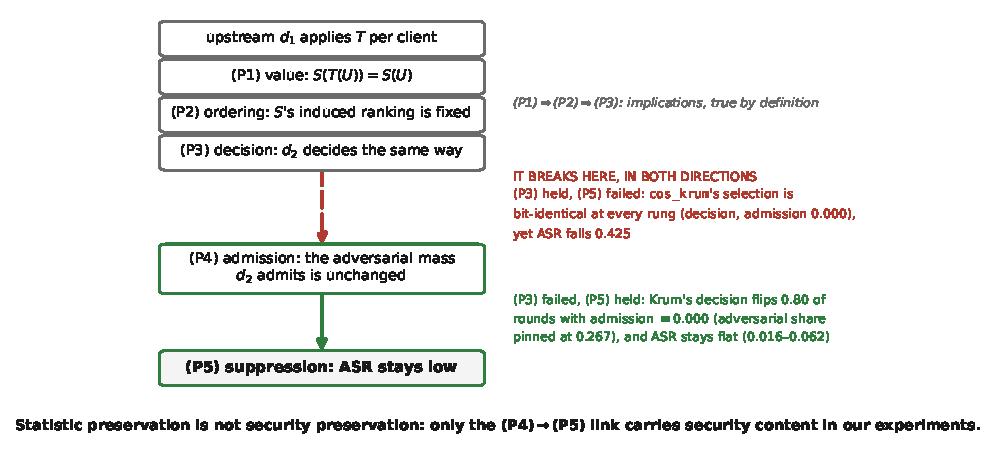
\includegraphics[width=0.98\linewidth]{figures/story_chain.pdf}
\caption{\textbf{The preservation chain, and where it breaks.} (P1)$\Rightarrow$(P2)$\Rightarrow$(P3)
holds by definition; \textbf{below (P3) the chain breaks, in both directions}, and both witnesses come
from the oracle intervention that pins every adversary's coefficient and so closes
Lemma~\ref{lem:annihilation}'s attenuation channel \emph{by construction} (\S\ref{sec:targeted}).
The pooled statistic-level prediction we had frozen is separately \textbf{rejected} by a
pre-registered ladder (\S\ref{sec:dose_response}), and a pre-registered replication in a different
invariance class reproduces the negative but \textbf{refutes the cross-arm admission ordering}, so
\textbf{admission is more causally proximal than the statistic, and not a validated predictor}. Every number in the figure is
recomputed from the scoring scripts' own JSON by \texttt{story\_chain\_figure.py}.}
\label{fig:story}
\end{figure}

\begin{figure}[t]
\centering
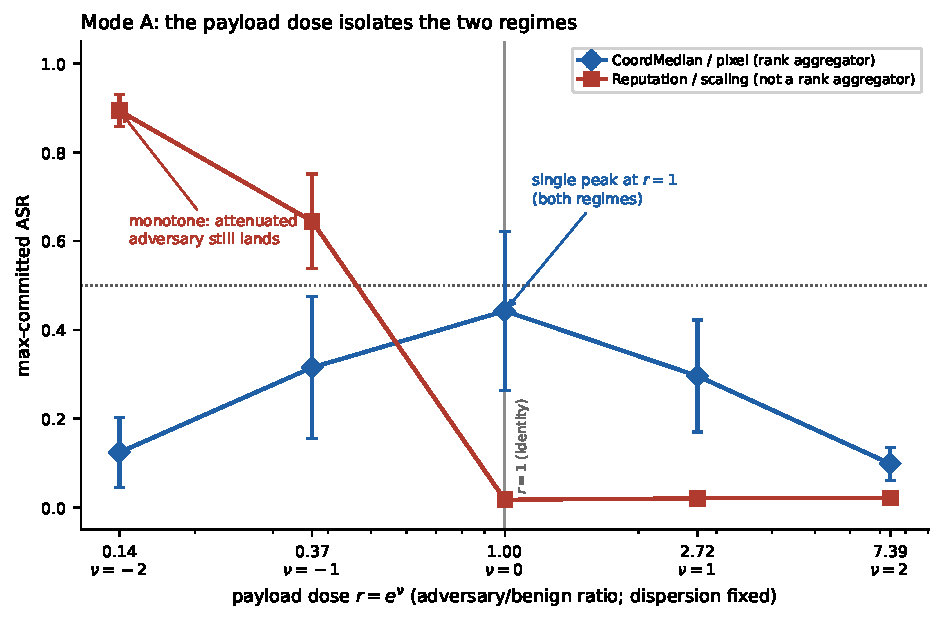
\includegraphics[width=0.70\linewidth]{figures/targeted_modeA.pdf}
\caption{\textbf{The two regimes, exhibited: the payload dose separates them.} \emph{The picture of regimes A and B of \S\ref{sec:framework}, produced by the instrument of \S\ref{sec:targeted_rest}.} With the statistic's dispersion fixed and only the adversary/benign weight ratio $r$ swept, \texttt{coord\_median} (a rank aggregator, the class the regimes are stated for) is single-peaked at $r{=}1$ as Theorem~\ref{thm:bounded_reweight} predicts, while reputation is monotone: off-spec, and the theorem is not claimed for it. Bars are Student-$t$ $95\%$ intervals, recomputed per seed by \texttt{analyze\_targeted\_dose.py}; the Mode-S companion is Table~\ref{tab:targeted}.}
\label{fig:modeA}
\end{figure}

Table~\ref{tab:dose_perseed} is every cell of the ladder; Figure~\ref{fig:dose_measured} plots it on the measured axis and Figure~\ref{fig:dose_ladder} on the nominal one. Both are produced by \texttt{analyze\_dose\_response.py} and \texttt{dose\_response\_figure.py} from \texttt{results/dose\_response/}; nothing below is transcribed from a log.

\paragraph{The replication arm's post-hoc seed-matched difference.} The frozen primary for the \texttt{coord\_median} replication (\S\ref{sec:targeted}) is the \emph{unpaired} $\Delta = +0.098$, and it is not superseded by what follows. Between-seed variance on this cell is large (identity ASR spread $0.287$--$0.677$), which the unpaired test cannot see through, so we also report the seed-matched difference: positive in $5/5$ seeds, paired $t = 3.39$, one-sided $p = 0.014$. \textbf{This is post-hoc and was not pre-registered}; we report it because it is the honest description of a small consistent effect, and we label it post-hoc wherever it appears. It does not change the frozen verdict: the admission \emph{ordering} is refuted either way.

\begin{figure}[h]
\centering
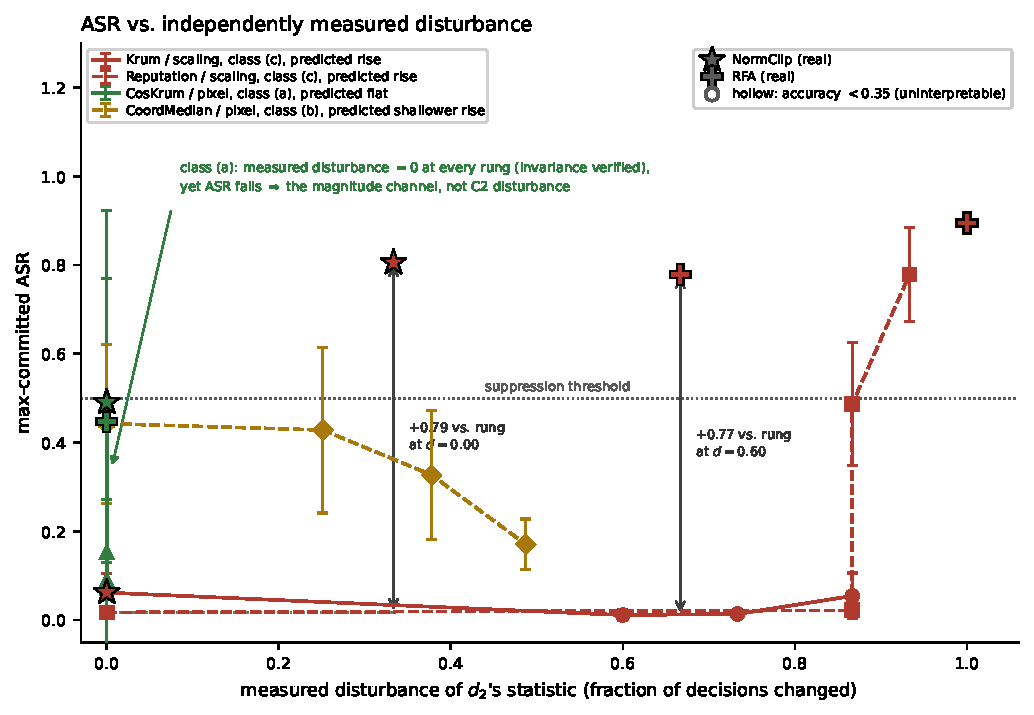
\includegraphics[width=0.62\linewidth]{figures/dose_measured.pdf}
\caption{\textbf{The measured axis: ASR against disturbance of each arm's own statistic}, an abscissa fixed before the freeze ($n{=}5$, Student-$t$ 95\% intervals; the figure script imports the arm and anchor construction from the scoring script, so the two cannot diverge). Stars and crosses are the two \emph{real} upstream transforms measured on these same cells: at matched disturbance they sit $+0.77$ and $+0.79$ ASR \emph{above} the synthetic curve, though their realized weight ratios (mean $3.61$ and $11.93$, maximum $4.90$ and $17.38$) lie \emph{inside} the ladder's span; \S\ref{sec:dose_response} attributes the gap to $\Delta_c$, post-hoc. The class-(a) arm's four rungs coincide at disturbance exactly $0$ and its ASR falls anyway: Lemma~\ref{lem:annihilation}'s magnitude channel, not C2 disturbance. Hollow markers fail the $0.35$ accuracy gate.}
\label{fig:dose_measured}
\end{figure}

\begin{figure}[h]
\centering
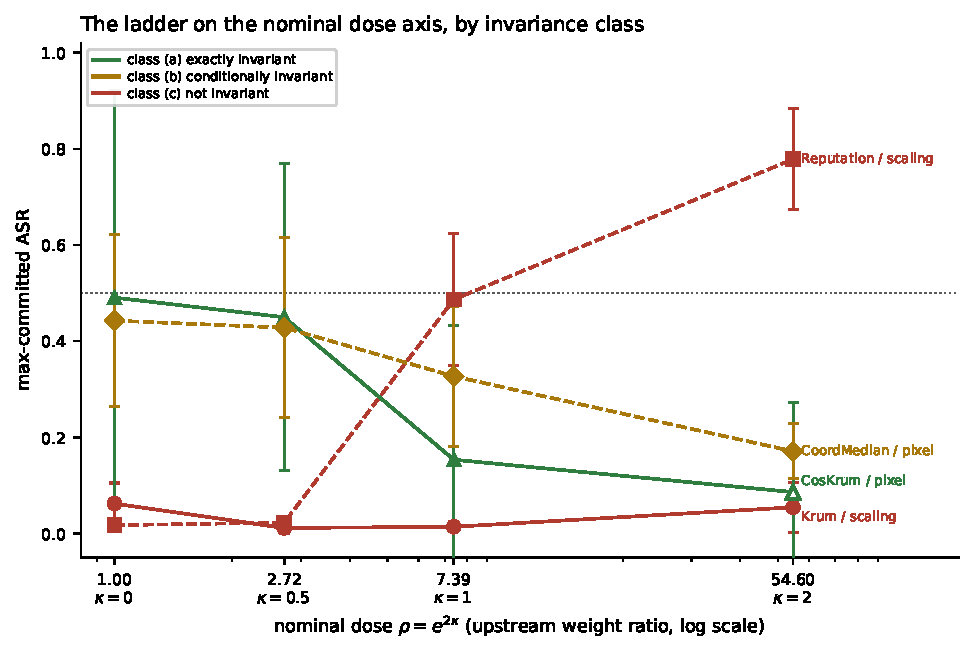
\includegraphics[width=0.62\linewidth]{figures/dose_ladder.pdf}
\caption{\textbf{The nominal axis}: the same 16 cells against the dose $\rho = e^{2\kappa}$, coloured by Proposition~\ref{prop:invariance} class. Of the two class-(c) arms the fragility claim is stated over, only reputation rises; the other two arms \emph{fall}. This is the axis the frozen per-arm shapes were stated on, and the pooled prediction was stated on the measured axis of Figure~\ref{fig:dose_measured}. Hollow markers fail the $0.35$ accuracy gate.}
\label{fig:dose_ladder}
\end{figure}

\begin{table}[h]
\caption{All 16 rungs, $n{=}5$. \emph{disturb} is the independently measured disturbance of that arm's own statistic at that rung, computed before the freeze with no ASR involved; \emph{rise} is ASR relative to the arm's own $\kappa{=}0$ rung and is the primary test's ordinate. CIs are Student-$t$ at $n{=}5$ and are wide by design: the ladder was powered to detect a monotone trend, not to resolve single cells. $^{\dagger}$ fails the $0.35$ clean-accuracy gate.}
\label{tab:dose_perseed}
\centering\scriptsize\setlength{\tabcolsep}{2.5pt}
\begin{tabular}{llrrrcrrrrrrr}
\toprule
\textbf{arm} & $\kappa$ & $\rho$ & \textbf{dist.} & \textbf{ASR} & \textbf{95\% CI} & \textbf{rise} & \textbf{acc} & \multicolumn{5}{c}{\textbf{per-seed ASR (42--46)}} \\
\midrule
\texttt{krum} & $0$ & $1.00$ & $0.000$ & $0.062$ & $[0.019, 0.105]$ & $+0.000$ & $0.565$ & $0.115$ & $0.021$ & $0.047$ & $0.057$ & $0.069$ \\
scaling & $0.5$ & $2.72$ & $0.600$ & $0.011$ & $[-0.001, 0.023]$ & $-0.051$ & $0.652$ & $0.000$ & $0.010$ & $0.011$ & $0.027$ & $0.007$ \\
class (c) & $1.0$ & $7.39$ & $0.733$ & $0.014$ & $[0.003, 0.024]$ & $-0.048$ & $0.682$ & $0.003$ & $0.015$ & $0.021$ & $0.021$ & $0.008$ \\
 & $2.0$ & $54.60$ & $0.867$ & $0.054$ & $[0.002, 0.106]$ & $-0.008$ & $0.619$ & $0.005$ & $0.039$ & $0.077$ & $0.113$ & $0.037$ \\
\midrule
\texttt{reputation} & $0$ & $1.00$ & $0.000$ & $0.017$ & $[0.012, 0.022]$ & $+0.000$ & $0.777$ & $0.014$ & $0.012$ & $0.017$ & $0.023$ & $0.019$ \\
scaling & $0.5$ & $2.72$ & $0.867$ & $0.022$ & $[0.014, 0.031]$ & $+0.005$ & $0.779$ & $0.016$ & $0.018$ & $0.024$ & $0.033$ & $0.020$ \\
class (c) & $1.0$ & $7.39$ & $0.867$ & $0.487$ & $[0.349, 0.624]$ & $+0.470$ & $0.765$ & $0.439$ & $0.547$ & $0.578$ & $0.557$ & $0.313$ \\
 & $2.0$ & $54.60$ & $0.933$ & $0.779$ & $[0.673, 0.885]$ & $+0.762$ & $0.701$ & $0.710$ & $0.843$ & $0.730$ & $0.896$ & $0.714$ \\
\midrule
\texttt{cos\_krum} & $0$ & $1.00$ & $0.000$ & $0.490$ & $[0.058, 0.922]$ & $+0.000$ & $0.607$ & $0.003$ & $0.269$ & $0.630$ & $0.864$ & $0.686$ \\
pixel & $0.5$ & $2.72$ & $0.000$ & $0.450$ & $[0.130, 0.769]$ & $-0.041$ & $0.569$ & $0.764$ & $0.236$ & $0.165$ & $0.648$ & $0.435$ \\
class (a) & $1.0$ & $7.39$ & $0.000$ & $0.153$ & $[-0.127, 0.433]$ & $-0.337$ & $0.466$ & $0.132$ & $0.090$ & $0.000$ & $0.543$ & $0.001$ \\
 & $2.0$ & $54.60$ & $0.000$ & $0.086$ & $[-0.100, 0.271]$ & $-0.405$ & $0.220^{\dagger}$ & $0.083$ & $0.000$ & $0.000$ & $0.345$ & $0.000$ \\
\midrule
\texttt{coord\_median} & $0$ & $1.00$ & $0.000$ & $0.443$ & $[0.263, 0.622]$ & $+0.000$ & $0.767$ & $0.395$ & $0.287$ & $0.449$ & $0.677$ & $0.405$ \\
pixel & $0.5$ & $2.72$ & $0.251$ & $0.428$ & $[0.241, 0.615]$ & $-0.015$ & $0.764$ & $0.454$ & $0.215$ & $0.430$ & $0.638$ & $0.402$ \\
class (b) & $1.0$ & $7.39$ & $0.378$ & $0.327$ & $[0.181, 0.472]$ & $-0.116$ & $0.749$ & $0.351$ & $0.139$ & $0.352$ & $0.463$ & $0.328$ \\
 & $2.0$ & $54.60$ & $0.487$ & $0.170$ & $[0.113, 0.228]$ & $-0.272$ & $0.690$ & $0.179$ & $0.090$ & $0.204$ & $0.192$ & $0.187$ \\
\bottomrule
\end{tabular}
\end{table}

\paragraph{The primary test, and two post-hoc sensitivities that cannot change its verdict.} The frozen primary test is a one-sided Spearman correlation of \emph{rise} against \emph{measured disturbance} pooled over all 16 cells, confirmed only at $\rho_s > 0$ with $p < 0.05$: we obtain $\rho_s = +0.351$, $p = 0.091$, so it is \textbf{refuted}. Two sensitivities are recorded because they are informative about \emph{why}, and are labelled post-hoc because neither was frozen. (i) The four $\kappa{=}0$ cells are constructed $(0,0)$ points (zero disturbance and zero rise by definition) and dropping them gives $\rho_s = +0.780$, $p = 0.001$ ($n{=}12$); so the pooled correlation is carried by the arm-2 rise and destroyed by the two arms whose ASR falls, not by the identity anchors. (ii) Against the \emph{nominal} dose $\kappa$ (i.e.\ $\log \rho$) rather than measured disturbance, $\rho_s = -0.354$, $p = 0.911$: the wrong sign, which is the same fact as three arms falling. Neither is scored.

\paragraph{Per-arm trend tests.} One-sided Jonckheere--Terpstra across the four ordered rungs, $5$ seeds each, $\alpha = 0.05$; the normal-approximation $p$ agrees with a $20{,}000$-draw permutation $p$ to three decimals throughout. Arm 1: $J = 70$, $z = -0.34$, $p_{\uparrow} = 0.632$. Arm 2: $J = 144$, $z = +4.64$, $p_{\uparrow} = 1.7{\times}10^{-6}$. Arm 3: $J = 29$, $z = -3.10$, $p_{\uparrow} = 0.999$ ($p_{\downarrow} = 9.8{\times}10^{-4}$); dropping the gated $\kappa{=}2.0$ rung leaves $z = -2.06$, $p_{\downarrow} = 0.020$, so the decrease is not an artifact of the collapsed cell alone. Arm 4: $J = 31$, $z = -2.96$, $p_{\uparrow} = 0.998$ ($p_{\downarrow} = 1.5{\times}10^{-3}$). No frozen rule tests the decreasing direction; $p_{\downarrow}$ is descriptive.

\paragraph{Clean accuracy against dose separates two ways of losing ASR.} Descriptive, not pre-registered. Accuracy trends by the same test: arm 1 $z = +1.35$, arm 2 $z = -3.30$, arm 3 $z = -3.50$, arm 4 $z = -4.11$. Arm 3 pays $0.607 \to 0.220$: a $0.39$ collapse through the Lemma~\ref{lem:annihilation} contraction channel, and the reason its $\kappa{=}2.0$ cell is uninterpretable rather than a success. Arm 4 pays only $0.767 \to 0.690$ while ASR more than halves, so there the dose genuinely \emph{helps} coordinate median: a refutation of our predicted shape, but a benign mechanism. Arm 2 is the cleanest cell in the ladder, losing $0.076$ accuracy while ASR rises $46\times$.

\paragraph{Anchor residuals, and why the instrument is the finding.} Residual is real-transform ASR ($n{=}5$, from \texttt{metric\_swap\_topup}) minus the synthetic rung at the nearest measured disturbance. NormClip$\to$Krum: disturbance $0/9$, ASR $0.062$ vs.\ rung $0.062$, residual $+0.001$. RFA$\to$Krum: $6/9 = 0.667$, ASR $0.779$ vs.\ rung $0.011$ at disturbance $0.600$, residual $\mathbf{+0.767}$. NormClip$\to$Reputation: $3/9 = 0.333$, ASR $0.806$ vs.\ rung $0.017$, residual $\mathbf{+0.789}$. RFA$\to$Reputation: $9/9$, $0.895$ vs.\ $0.779$, residual $+0.116$. Both \texttt{cos\_krum} anchors sit at disturbance $0$ and land ($+0.000$, $-0.044$). \texttt{coord\_median} was not in the metric-swap menu, so arm 4 has \emph{no} real-transform anchor and its ecological validity is untested. The two large residuals are not a range mismatch: realized $\rho$ is mean $3.61$ / max $4.90$ for NormClip and mean $11.93$ / max $17.38$ for RFA, both inside the ladder's $[1.00, 54.60]$ span. What differs is \emph{which} clients get reweighted (NormClip and RFA reweight in a way correlated with adversary status, our permutation deliberately does not) and we state that as the hypothesis caveat~(iii) was written to test, not as a measured quantity: the shipped disturbance logs record only $c_{\min}$, $c_{\max}$ and $\rho$ per round, not per-client coefficients, so an adversary-versus-benign coefficient contrast requires a new (cheap, no-ASR) measurement.

\paragraph{Two checks that passed.} The $\kappa{=}0$ rung reproduces each arm's published standalone value exactly on every shared seed (16 seed-level comparisons across four arms, largest $|\Delta\text{ASR}|$ and $|\Delta\text{acc}|$ both $0.00\text{e}{+}00$ at tolerance $10^{-6}$), so $\kappa{=}0$ really is the identity and the fresh rung and the published baseline are the same quantity. \textbf{The first-rung fall we rest the (P4)$\not\Rightarrow$(P5) witness on}, in full: \texttt{cos\_krum} / pixel at $\rho{=}2.72$ falls $0.173$ with clean accuracy moving only $0.599 \to 0.567$, paired $t{=}{-}1.976$, one-sided $p{=}0.044$, falling in $5/8$ seeds. And \texttt{cos\_krum}'s selection never changed in any of the $120$ measured cells, with maximum relative score drift $1.1{\times}10^{-4}$: Proposition~\ref{prop:invariance}'s classification of which statistics a positive per-client rescaling can disturb is verified directly, independently of the outcome the ladder then failed to predict.

\section{Secondary results: baselines, the adaptive stress test, scale, and switching}
\label{app:secondary}

\paragraph{The margin behaves like a certificate, not just a switch.} C3 is binary, but the margin $m$ is measurable and its \emph{strength} tracks security: over the 29 measured rounds with $w_a>0$, higher margin goes with lower realized adversarial mass (Spearman $\rho = -0.48$, $p = 0.009$), Corollary~\ref{cor:aggregate_mass}'s bound holding in every one, a number rather than a verdict, though the link is directional, not fitted, and post-hoc.

\begin{figure}[t]
\centering
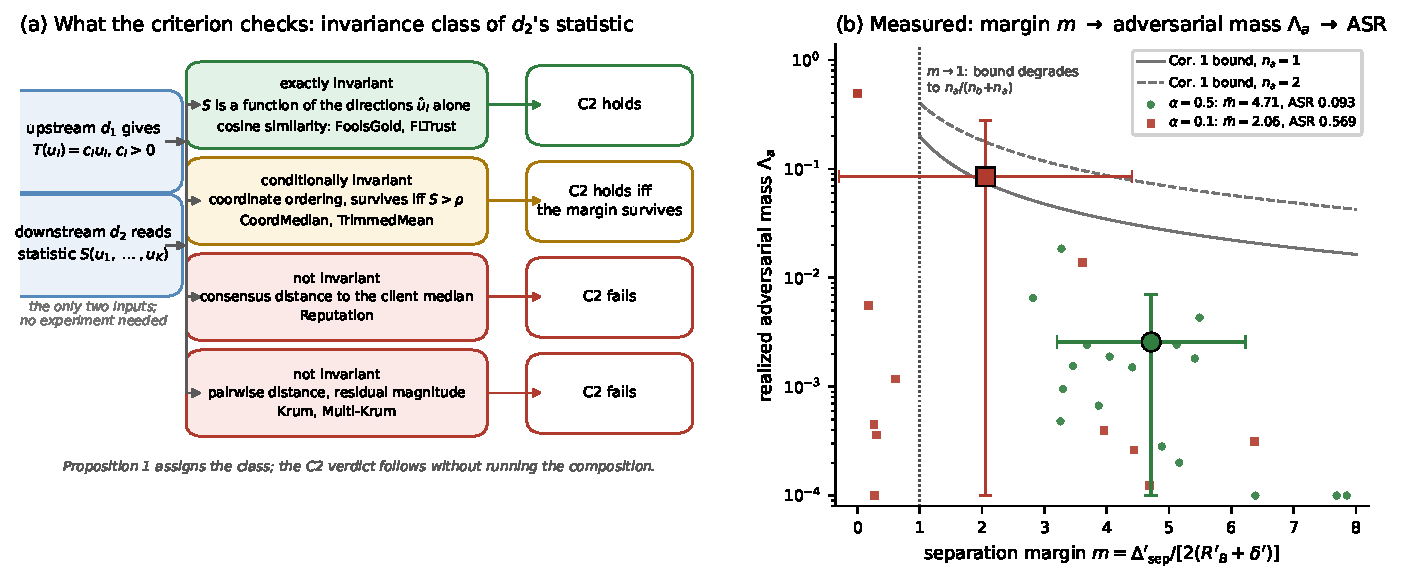
\includegraphics[width=0.84\linewidth]{figures/mechanism_chain.pdf}
\caption{\textbf{The criterion is a mechanism test, and the mechanism is measurable.}
\textbf{(a)} What C2 checks: the upstream transform $T$ and the statistic $S$ that $d_2$ reads
determine an \emph{invariance class} (Proposition~\ref{prop:invariance}), and the class
determines the verdict with no composition run, which is why norm clipping does not blind
FoolsGold but does blind Reputation.
\textbf{(b)} The measured chain for FG$\to$RFA, per round, on the transformed points RFA
actually receives; each marker is one round with $w_a>0$ (rounds where FoolsGold zeroes every
adversary are Lemma~\ref{lem:annihilation} and carry no payload), large markers are
mean~$\pm$~s.d., and values below $10^{-4}$ are drawn at $10^{-4}$.
Corollary~\ref{cor:aggregate_mass}'s bound holds in every round, and the $\alpha{=}0.1$
collapse is visible in the theorem's own quantity: $m$ falls from $4.71 \pm 1.51$ ($n{=}17$)
to $2.06 \pm 2.35$ ($n{=}12$), with several rounds at $m{<}1$ where the bound degrades to
$n_a/(n_b{+}n_a)$, and realized $\Lambda_a$ rises $0.003 \to 0.085$ (max $0.50$) as
composition ASR goes $0.093 \to 0.569$.}
\label{fig:mechanism}
\end{figure}

\begin{table}[h]
\caption{Framework validation (representative pairs; full tallies in text). Threshold: LOW $< 0.5$, HIGH $\geq 0.5$.}
\label{tab:validation}
\centering\small
\begin{tabular}{lcccc}
\toprule
\textbf{Composition} & \textbf{Category} & \textbf{Predicted} & \textbf{Max ASR} & \textbf{Correct?} \\
\midrule
\multicolumn{5}{l}{\emph{PASS: C1$\wedge$C2$\wedge$C3 (predicted LOW)}} \\
FoolsGold $\to$ RFA & PASS & LOW & $0.093$ & \checkmark \\
FoolsGold $\to$ CoordMedian & PASS & LOW & $0.107$ & \checkmark \\
Reputation $\to$ CoordMedian & PASS & LOW & $0.423$ & \checkmark \\
\midrule
\multicolumn{5}{l}{\emph{C1-FAIL: no constituent suppresses (predicted HIGH)}} \\
Reputation $\to$ RFA & C1-FAIL & HIGH & $0.825$ & \checkmark \\
NormClip $\to$ FoolsGold$^\dagger$ & C1-FAIL & HIGH & $0.887$ & \checkmark \\
RFA $\to$ FoolsGold$^\dagger$ & C1-FAIL & HIGH & $0.914$ & \checkmark \\
\midrule
\multicolumn{5}{l}{\emph{C2-FAIL: discriminative property destroyed (predicted HIGH)}} \\
NormClip $\to$ Reputation & C2-FAIL & HIGH & $0.819$ & \checkmark \\
\midrule
\multicolumn{5}{l}{\emph{C3-FAIL: margin compressed (predicted HIGH)}} \\
FoolsGold $\to$ TrimmedMean & C3-FAIL & HIGH & $0.508$ & \checkmark \\
NormClip $\to$ RFA & C3-FAIL & HIGH & $0.853$ & \checkmark \\
\midrule
\multicolumn{5}{l}{\emph{False negatives (predicted HIGH, measured LOW)}} \\
NormClip $\to$ CM \,/\, RFA $\to$ CM & C3-FAIL & HIGH & $0.433$ \,/\, $0.485$ & $\times$ \\
\bottomrule
\multicolumn{5}{l}{\footnotesize $^\dagger$Reclassified from C2-FAIL: by Proposition~\ref{prop:invariance}(a) these preserve C2.} \\
\end{tabular}
\end{table}

\paragraph{Single-defense baselines.} Measured under the identical protocol (5 seeds, 50 rounds), no individual defense achieves low max-committed ASR: CM 0.52, FG 0.73, Rep 0.84, TM 0.85, RFA 0.89, NC 0.94. Against the best single defense (CM, 0.52), FG$\to$RFA (0.093) is $5.6\times$ lower and FG$\to$CM (0.107) is $4.9\times$ lower. FoolsGold alone reaches ASR 0.20 on model-scaling only by collapsing the model to 10\% accuracy, so it is not suppression: consistent with its C1 failure.

\paragraph{Adaptive attacks against FG$\to$RFA.} We evaluate one whitebox adaptive attack family that jointly evades both defenses: disjoint coordinate blocks minimize cosine similarity (evade FG) while $\epsilon$-ball projection stays near the geometric median (evade RFA). The adversary has full state access, and these constraints are in tension. ASR against FG$\to$RFA (5 seeds each, base quoted on the \emph{same} five seeds \emph{and the same pixel attack the adaptive family is built from}, so the comparison is seed-matched and same-attack rather than against the $n{=}30$ mean or the pairs worse scaling arm): base committed pixel $0.045 \pm 0.013$; Neurotoxin~\citep{zhang2022neurotoxin} top-20\% at scale 2.0 $0.048 \pm 0.009$; projection only, no decorrelation, $\epsilon{=}2$: $0.050 \pm 0.008$. With joint constraints the sweep over $\epsilon$ gives $0.036 \pm 0.015$ ($\epsilon{=}0.5$), $\mathbf{0.167 \pm 0.069}$ ($\epsilon{=}1$), $0.130 \pm 0.030$ ($\epsilon{=}2$), $0.124 \pm 0.025$ ($\epsilon{=}4$). ASR peaks at $\epsilon{=}1$: tighter projection over-constrains the attack, larger $\epsilon$ fails to evade RFA, and without decorrelation FoolsGold suppresses it outright, so the competing constraints leave a narrow effective window. This is an empirical finding (Theorem~\ref{thm:bounded_reweight} concerns mechanism preservation and does not bound an adaptive adversary whose optimization is untied to its conditions) and it probes one natural family of joint constraints at a handful of $\epsilon$ values, not the adaptive attack space. Within it, $0.167$ is $3.7\times$ the seed-matched committed-pixel ASR ($2.6\times$ the $n{=}30$ pixel mean of $0.064$; against the pairs scaling arm, which the adaptive family does not attack, the ratios would read $3.3	imes$ and $1.8	imes$).

\paragraph{Scale.} At $N{=}100$, $f{=}0.05$, ResNet18 both pre-registered PASS predictions hold: FG$\to$RFA max ASR $= 0.069$, FG$\to$CM $= 0.152$. We flag that these runs reach only ${\approx}0.29$ clean accuracy at 50 rounds (ResNet18 is far from converged at this budget), so they establish that suppression transfers across scale and architecture, not that the composition is deployable at $N{=}100$ as configured.

\subsection{Heterogeneity, and where the criterion breaks}
\label{app:alpha_sweep}
Earlier drafts swept heterogeneity for single defenses only; no composition had been run at any $\alpha \neq 0.5$. We therefore ran all three PASS pairs across $\alpha \in \{0.1, 1.0, 10.0\}$ (3 seeds, both attacks, 50 rounds; max-committed ASR / clean accuracy):

\begin{center}\small
\begin{tabular}{lcccc}
\toprule
\textbf{Composition} & $\alpha{=}0.1$ & $\alpha{=}0.5$ & $\alpha{=}1.0$ & $\alpha{=}10.0$ \\
\midrule
FG$\to$RFA & \textbf{0.569} / 0.20 & 0.093 / 0.50 & 0.051 / 0.57 & 0.063 / 0.62 \\
FG$\to$CM & 0.433 / 0.40 & 0.107 / 0.68 & 0.133 / 0.74 & 0.129 / 0.78 \\
Rep$\to$CM & \textbf{0.548} / 0.48 & 0.423 / 0.76 & 0.377 / 0.79 & 0.326 / 0.81 \\
\bottomrule
\end{tabular}
\end{center}

\noindent In our sweep, which is three seeds per cell and fixes direction rather than magnitude, the certified compositions stay below threshold for $\alpha \in \{0.5, 1.0, 10.0\}$, including the near-IID setting where one might expect FoolsGold to founder on legitimately similar benign updates: $\alpha{=}10$ is indistinguishable from $\alpha{=}0.5$. \textbf{Under extreme heterogeneity ($\alpha{=}0.1$) two of the three PASS compositions cross the threshold} (FG$\to$RFA $0.569$, Rep$\to$CM $0.548$) and only FG$\to$CM survives, at $0.433$: a real boundary condition on the framework, with caveats in both directions: FG$\to$RFA at $\alpha{=}0.1$ is strongly bimodal across seeds ($0.065$--$0.923$), so at $n{=}3$ the direction is clear but the magnitude is not, and clean accuracy degrades badly ($0.20$--$0.48$), so the regime stresses utility as well as security. Crucially Theorem~\ref{thm:bounded_reweight} supplies a diagnostic quantity that retrospectively explains this boundary: re-measuring the transformed points at $\alpha{=}0.1$, RFA's separation margin $m := \Delta'_{\mathrm{sep}}/[2(R'_B+\delta')]$ collapses from an all-round mean of $3.24$ (met in 68\% of rounds) to $1.01$ (met in 20\%), over the payload-carrying rounds alone, the ones Figure~\ref{fig:mechanism} plots, the same collapse reads $4.71 \pm 1.51$ ($n{=}17$) to $2.06 \pm 2.35$ ($n{=}12$) with the per-round minimum falling $2.82 \to 0.00$, the difference being that the all-round means average in the Lemma~\ref{lem:annihilation} rounds at $m{=}0$, exactly the boundary $m \to 1$ where Corollary~\ref{cor:aggregate_mass}'s bound degrades to $40\%$ adversarial mass, because extreme heterogeneity inflates the benign radius $R'_B$ until the benign cluster is no longer separated from the adversarial points, which is the precondition the theorem requires. A practitioner running the 5--10 round pilot we recommend would measure $m \approx 1$ and decline to deploy. The criterion is therefore mechanistically diagnostic at this boundary (the property that makes a screening rule usable) though this is a post-hoc explanation of a known failure, not a pre-registered prediction of it.

\subsection{Composition vs.\ randomized switching}
\label{sec:mixing}

\paragraph{High persistence sharply reduces the value of temporal switching.} In our tested regime, $\gamma \approx 0.66$ ($\gamma := \text{ASR}(t{+}1)/\text{ASR}(t)$ after one clean round): triggers decay slowly enough that intermittent suppression cannot clear them, so temporal mixing approaches the weaker constituent defense's performance. Whether switching retains any value depends jointly on $\gamma$, injection strength, switching frequency, and recovery dynamics: persistence alone does not imply switching is worthless. The quantitative boundary is architecture-specific; the qualitative prediction (high-$\gamma$ attacks blunt switching) is what this secondary analysis contributes, and nothing in the preservation argument rests on it.

\paragraph{Order-sensitivity control.} Both variants apply both defenses every round and differ \emph{only} in order, so compute is matched and any gap is structural. We report it as a \textbf{motivating demonstration that composition order is structurally consequential, not as evidence for the criterion}: the mechanism behind the largest gap is a degeneracy rather than a signal-preservation failure, as the diagnosis below makes clear. Pixel ASR, 5 seeds: fixed FG$\to$CM $0.076 \pm 0.035$ versus randomized 50/50 ordering $0.681 \pm 0.133$ ($9\times$) and temporal mixing of one defense per round $0.679 \pm 0.159$; fixed FG$\to$RFA $0.037 \pm 0.011$ versus randomized $0.719 \pm 0.113$ ($19\times$). The mechanism is the degeneracy of §\ref{sec:intro}: CoordMedian supplies no per-client transform, so every CM$\to$FG round reduces to FoolsGold alone, leaving half the rounds defended by a single constituent that cannot suppress on its own. On a reputation+TrimmedMean menu ($n{=}30$), composition reaches ASR $0.316$ against $0.915$ for temporal mixing.

\section{The metric-swap suite's two-sided prediction}
\label{app:gate_prediction}

Because C1 binds for all eight pairs, every frozen label in the metric-swap suite was HIGH (a consequence of the measured inputs rather than a later choice), so the suite bears on specificity only. One prediction inside it was genuinely two-sided. \texttt{cos\_krum}'s C1 verdict on model-scaling turns on whether the accuracy gate is applied ($0.078$ ASR at $0.146$ clean accuracy), so we froze \emph{both} readings in advance: primary (gated) $\Rightarrow$ HIGH, secondary (numeric only) $\Rightarrow$ LOW, with the rule fixed beforehand that a LOW outcome at accuracy $\ge 0.35$ would mean the gate was wrong. Both cells came out \textbf{HIGH} ($0.508$, $0.566$), so the gate is vindicated against a pre-registered alternative that would have overturned it. This is the only place in the paper where our own accuracy gate was put at risk by a frozen rule.

\section{The prospective suite, arm by arm}
\label{app:prospective}

\textbf{(i) FLTrust as $d_1$ (7 pairs, 2/7): out of scope.} When $d_1$ alone suppresses, the composition inherits that suppression whatever $d_2$ does, so all five predicted-HIGH pairs are misses even though their C2/C3 failures are real: FLTrust genuinely destroys Reputation's consensus-distance signal, but destroying a mechanism that was never load-bearing costs nothing. This is C0, and it was invisible on the original 42 pairs, where the strongest single defense reaches only $0.519$ and the lowest ASR among all 39 non-PASS pairs is $0.433$; no pair was ever out of scope. We apply C0 here \emph{retrospectively}, which is weaker than a pre-registered exclusion.

\textbf{(ii) FLTrust as $d_2$ (6 pairs, 6/6): in scope, but nearly an identity.} Proposition~\ref{prop:invariance}(a) predicts $\cdot\to$FLTrust preserves C2, and it does, but FLTrust gates on a scale-invariant cosine and then \emph{renormalizes every update to $\|g_{\mathrm{srv}}\|$}, discarding magnitude outright, so a positive rescaling $u_i \mapsto c_i u_i$ is \emph{exactly} cancelled: FLTrust discards precisely what $d_1$ modifies. The per-seed data show this directly. Krum$\to$FLTrust and MKrum$\to$FLTrust are \textbf{bit-identical} to FLTrust alone on all six runs (pass-through $d_1$); NC$\to$FLTrust is bit-identical \emph{on the pixel attack}, where no client exceeds $\tau{=}5$ so $c_i \equiv 1$, and differs only within seed noise on model-scaling, where clipping fires; Rep$\to$ and RFA$\to$FLTrust likewise differ only within noise. The lone real deviation is FG$\to$FLTrust ($0.064$, up to $0.084$ per seed): the one $d_1$ producing exact \emph{zeros} rather than positive rescalings, changing FLTrust's client set instead of its magnitudes, which is the Lemma~\ref{lem:annihilation} interaction. So this arm confirms that theory and implementation agree, and demonstrates the degeneracy mechanism cleanly, but it is \textbf{not falsifiable}: every $d_1$ in our menu is a \emph{non-negative} per-client rescaling, FLTrust cancels the positive part exactly, and so the only channel left open is the \emph{zero pattern}, which is precisely where the one deviation appears. Proposition~\ref{prop:invariance}(a) permits no other outcome on the strictly-positive part, and Lemma~\ref{lem:annihilation} accounts for the rest.

\textbf{(iii) Neither defense is FLTrust (7 pairs, 5/7): the only arm that could have surprised us.} All were predicted HIGH; correct are rep$\to$krum $0.880$, nc$\to$mkrum $0.943$, rfa$\to$mkrum $0.875$, krum$\to$rfa and mkrum$\to$rfa both $0.870$. Of those five, only rep$\to$krum composes two real mechanisms: MultiKrum at $K{=}5$ is bit-identical to FedAvg, so nc$\to$mkrum and rfa$\to$mkrum are NormClip and RFA standalone, and krum$\to$rfa and mkrum$\to$rfa are one measurement of RFA standalone made twice (per-seed $|\Delta\mathrm{ASR}| = 0.000$). Neither miss is a mechanism error: fg$\to$krum reads $0.078$ at $9.9\%$ clean accuracy (a collapsed model, the same hollow-suppression artifact as FoolsGold alone) and krum$\to$cm reads $0.450$ against a $0.5$ threshold as a degenerate pair reducing to CoordMedian alone, whose own baseline is $0.519$: threshold noise on a borderline constituent. This arm contains \emph{zero} predicted-LOW pairs, so like Tier 2 it bears on specificity only.

\paragraph{The suggestive contrasts, withdrawn.} We had read three matched pairs, $d_1$ held fixed while $d_2$ moved from FLTrust to a Euclidean rule, as a $19$--$20\times$ gap turning on exactly the property Proposition~\ref{prop:invariance} identifies. Two of them ran against MultiKrum, which at $K{=}5$ selects \emph{all five} participants and is therefore bit-identical to FedAvg ($1.9\times10^{-6}$ per aggregation; a genuine selector again at $K{=}10$), so those arms carried no downstream defense at all. Substituting the genuine selector Krum does not repair them, and that is the finding: all three Krum arms take their max-committed ASR from the pixel backdoor, on which Krum's own standalone ASR is $0.583$, so the gap measures C1 failure rather than disturbed invariance, and nc$\to$krum is bit-identical to Krum alone on all three seeds because under that attack no client exceeds $\tau{=}5$ and $d_1$ is the exact identity. Counting the pass-through $d_1$ rows as well, $8$ of the $20$ rows reduce to a single defense rather than the $5$ labelled DEGEN at freeze, and arm (iii) composes two real mechanisms in $2$ pairs, not $7$. The frozen labels and the $13/20$ score stand; what we retract is our reading of them. The confound is accordingly worse than we reported, in the way Lemma~\ref{lem:testability} predicts: the invariant-signal $d_2$ is also the only $d_2$ in this menu that suppresses alone, so effectiveness and mechanism co-vary across the contrast. This is why breaking the confound requires holding standalone effectiveness fixed rather than choosing a different defense.

\section{Adversary-correlated dispersion $\Delta_c$, measured}
\label{app:delta_c}

\subsection{Heterogeneity is not the mechanism: $\rho$ against $\Delta_c$}
\label{sec:rho_vs_deltac}

\noindent \textbf{The finding, stated first.} What costs a downstream defense its suppression is not how heterogeneous the upstream transform is but \textbf{whether its reweighting is correlated with adversary identity}, and not even the size of that correlation, which has \textbf{two opposite regimes}. This is why our own headline predictor failed.

\paragraph{Two different things a coefficient vector does, and the theory sees only one.} (Symbols: Appendix~\ref{app:notation}.) Proposition~\ref{prop:invariance} turns on \textbf{dispersion}, $\rho := \max_i c_i/\min_i c_i$ (how far apart the coefficients are, which decides whether an ordering survives) and says nothing about \emph{which} clients receive which coefficient. That second property is \textbf{adversary-correlated dispersion},
\[
\Delta_c \;:=\; \mathbb{E}[c_i \mid i \in A] \;-\; \mathbb{E}[c_i \mid i \notin A],
\qquad A \text{ the adversarial participants,}
\]
and the two are \textbf{independently controllable}, not merely uncorrelated in our sample: a transform can spread the coefficients arbitrarily at $\Delta_c = 0$ exactly, or leave them nearly equal while shifting the adversary's share, and Proposition~\ref{prop:rho_deltac} exhibits a family of each. \textbf{Proposition~\ref{prop:invariance} and Theorem~\ref{thm:bounded_reweight} constrain $\rho$; Lemma~\ref{lem:annihilation}'s attenuation channel is about $\Delta_c$}, and \S\ref{sec:dose_response} finds the real transforms differ on the second. $\Delta_c$ is \emph{not} a screening quantity: computing it requires knowing $A$ (\S\ref{sec:conclusion}).

\paragraph{Two mechanism-preserving regimes, at opposite ends of $\rho$.} Lemma~\ref{lem:annihilation} is a second, independent route to suppression, and the two together explain all three PASS compositions. Let $r := w_a/\max_b w_b$ and $S$ be the attack's coordinate extremeness. \textbf{(A) Ordering preservation} keeps the adversary in the tail where a rank aggregator discards it ($S \cdot r > 1$). \textbf{(B) Attenuation} instead drives the adversarial transformed value \emph{inside} the benign spread, where it cannot be an extreme order statistic and its payload is scaled by $r$ ($S \cdot r \ll 1$; $r=0$ is exact annihilation). The hazard is $S \cdot r \approx 1$, and our two weighting defenses sit at opposite ends: FoolsGold's weights are bounded ($\rho \le 2.1$, $S\cdot r \ge 4.8$), regime A; Reputation's are wildly unbounded ($\rho$ mean $1.4{\times}10^{5}$) precisely \emph{because} it crushes the adversary ($S\cdot r = 0.017$), regime B. So Reputation$\to$CoordMedian violates the ordering condition by five orders of magnitude and still suppresses (Figure~\ref{fig:modeA}, App.~\ref{app:dose_detail}, exhibits both regimes). Hence $\rho$ does not order $\Delta_c$ (Proposition~\ref{prop:rho_deltac}), and $\Delta_c$'s \emph{magnitude} does not order suppression either, the same large $|\Delta_c|$ being protective at one end and catastrophic at the other. \textbf{Neither quantity is a predictor}; they buy an account of \emph{why} a heterogeneity-based reading mispredicts.

$\Delta_c := \mathbb{E}[c_i \mid i \in A] - \mathbb{E}[c_i \mid i \notin A]$ for every per-client transform in the paper, over the same $5$ seeds $\times$ $3$ rounds and, within a round, the \emph{same} raw update stack for every transform, so the rows are comparable by construction (\texttt{measure\_coefficient\_targeting.py}, \texttt{results/coefficient\_targeting.json}). \textbf{No ASR is computed and no model is trained per transform}, which is what lets this be added without rescoring anything; the figures are \textbf{post-hoc and exploratory} and no frozen prediction depends on them. Coefficients are read back from transformed norms, $c_i = \|T(u_i)\|/\|u_i\|$, so Table~\ref{tab:delta_c} measures the shipped code path rather than the builder's description of it. As a provenance check the synthetic families' adversarial coefficient shares reproduce \texttt{results/admission\_measurement.json} to $0.0$ absolute on all 13 cells, so these rows may be read on the same axis as the Mode-S and Mode-A figures of \S\ref{sec:targeted}.

\begin{table}[h]
\centering\small\setlength{\tabcolsep}{4pt}
\caption{$\rho$ says how much a transform spreads the coefficients; $\Delta_c$ says who receives the spread. They are not ordered together: RFA and NormClip target the adversary $2$--$3.6\times$ harder than the ladder's most dispersed rung at $\rho$ that is $3.7$--$13\times$ \emph{smaller}. Means over non-degenerate rounds; the synthetic rows are attack-pooled since their coefficients do not depend on the attack.}
\label{tab:delta_c}
\begin{tabular}{@{}llrrrr@{}}
\toprule
\textbf{transform} & \textbf{attack} & $\rho$ & $\mathbb{E}[c \mid A]$ & $\mathbb{E}[c \mid \neg A]$ & $\Delta_c$ \\
\midrule
NormClip & model-scaling & $4.19$ & $0.268$ & $0.989$ & $-0.721$ \\
NormClip & pixel & $1.00$ & $1.000$ & $1.000$ & $0.000$ \\
Reputation & model-scaling & $8.3{\times}10^{5}$ & $0.003$ & $1.387$ & $-1.383$ \\
Reputation & pixel & $1.68$ & $0.915$ & $1.019$ & $-0.105$ \\
FoolsGold & model-scaling & $1.9{\times}10^{12}$ & $1.497$ & $0.834$ & $\mathbf{+0.663}$ \\
FoolsGold & pixel & $1.8{\times}10^{12}$ & $1.365$ & $0.986$ & $\mathbf{+0.378}$ \\
RFA & model-scaling & $14.8$ & $0.125$ & $1.332$ & $-1.208$ \\
RFA & pixel & $1.69$ & $0.923$ & $1.012$ & $-0.089$ \\
\midrule
\multicolumn{6}{@{}l@{}}{\emph{Synthetic families of \S\ref{sec:dose_response}--\S\ref{sec:targeted}, same code path:}} \\
ladder, $\kappa{=}0.5/1.0/2.0$ & --- & $2.72/7.39/54.6$ & --- & --- & $-0.140/{-}0.240/{-}0.336$ \\
Mode~S, all rungs & --- & $1.00$--$54.6$ & --- & --- & $\mathbf{0.000}$ \\
Mode~A, $\nu{=}{-}2\ldots{+}2$ & --- & $7.39$--$7.39$ & --- & --- & $-1.138 \ldots +2.469$ \\
\bottomrule
\end{tabular}
\end{table}

\noindent Three readings, in decreasing confidence. \textbf{(1) $\rho$ is not a proxy for $\Delta_c$}: the two are anti-ordered on the anchors, and NormClip on the pixel backdoor has $\rho = 1$ exactly because no client exceeds $\tau{=}5$, so $\Delta_c = 0$ there for a reason the invariance classification cannot see. \textbf{(2) Both transforms carrying a missed anchor are targeted far beyond any ladder rung}, which puts the residuals of \S\ref{sec:dose_response} on a measured axis rather than a range mismatch; $\Delta_c$ does not sort the anchors themselves, since NormClip carries one that misses and one that lands. \textbf{(3) $\Delta_c$ is nonetheless not a predictor of suppression}: RFA is strongly negative at $-1.208$ and rfa$\to$krum fails at $0.779$, while Reputation is more negative still at $-1.383$ and rep$\to$coord\_median suppresses. That is the two-regime structure of \S\ref{sec:framework} again: strong negative $\Delta_c$ can mean either annihilation or mere dilution, and $\Delta_c$'s magnitude alone does not say which. We report it as the axis on which the ladder's anchors were unmatched, not as the quantity that replaces the statistic.

\section{Confusion matrix in full}
\label{app:confusion}

Exactly 5 of the 42 pairs have max-committed ASR $< 0.5$: the 3 PASS pairs plus the 2 false negatives, all of which appear among the representative rows of Table~\ref{tab:validation}. Pooling both in-distribution tiers (each pair scored against the label committed for it at the time) gives TP${}=3$, FP${}=2$, TN${}=35$, FN${}=2$ (38/42; specificity 94.6\%, which we report but do not lead with, since 37 of 42 pairs are negatives and specificity is inflated by that imbalance; precision $1.0$ at base rate $11.9\%$ is the $8.4\times$ enrichment that matters, and recall is 40\% under the tightened C1, since FG$\to$RFA now counts as a miss). We report this pooled figure with its decomposition rather than on its own, because the tiers are not equivalent evidence: it is 16/18 development \emph{fit} plus 22/24 held-out \emph{prediction}. The four sub-tiers the body refuses to pool are development \emph{fit}, held-out \emph{specificity}, out-of-sample \emph{positives with no informative negatives}, and the 13/20 \emph{prospective} suite. Scoring instead against the criterion's mechanism labels, which classify both failed LOW calls as HIGH, gives TP${}=3$, FP${}=0$, TN${}=37$, FN${}=2$ (40/42); we take the more conservative pooled figure as primary. The two false positives, fg$\to$NC ($0.927$) and fedavg$\to$CM ($0.519$), were hedged as speculative at pre-registration time and neither satisfies C1; every pair that actually satisfies C1$\wedge$C2$\wedge$C3 came out LOW. Category tally after the Proposition~\ref{prop:invariance} correction: degenerate 18, C1-fail 11, C2-fail 3, C3-fail 7, PASS 3, and all 3 surviving C2 failures are $\cdot \to$ Reputation, exactly the non-invariant class of Proposition~\ref{prop:invariance}(c). With a positive set of only 2 certified in-distribution pairs and recall 40\%, the 94.6\% specificity figure is high partly because the positive class is rare, so we report it as a supporting statistic rather than a headline. The conditions are sufficient, not necessary, and they do reject working compositions. Extension to 3-way compositions: 9/10 triples correct (too small for confidence).

\section{Diagnosing the two false negatives in full}
\label{app:false_negatives}

NormClip$\to$CM ($0.433$) and RFA$\to$CM ($0.485$) were labelled C3-FAIL on the reading that \emph{any} heterogeneous upstream rescaling compresses a rank aggregator's margin. Theorem~\ref{thm:bounded_reweight}(1) says something weaker and quantitative: ordering survives when the attack's coordinate extremeness exceeds the realized weight ratio, $S > \rho$. Measured, NormClip's ratio is mild. Over 9 live rounds it clips only $0$--$2$ of 5 clients (11 of 45 client-rounds), so ${\approx}76\%$ of clients receive $c_i = 1$ \emph{exactly}, and the largest raw norm we observe is $24.5$ against $\tau{=}5$, bounding $\rho \leq 4.9$; against $S{=}10$ the margin $S/\rho \geq 2.0$ still clears $1$. RFA-reweighting is likewise near-uniform on benign clients. Both pairs therefore sit close to the \emph{uniform} rescaling case, where ordering is preserved exactly, which is why their ASR lands in an intermediate band just under threshold rather than in the high band the binary label predicts. \textbf{The refinement does not recover them.} Both also fail C1: CoordMedian alone is already at $0.519$, and neither NormClip ($0.935$) nor RFA ($0.885$) suppresses, so no reading of C3 makes either pair certifiable. What the diagnosis buys is a sharper condition and an account of the residual: a $d_2$ whose own baseline sits at $0.519$ needs only a mild order-preserving upstream transform to cross $0.5$, so these two are threshold noise around a marginal aggregator, not suppression the framework failed to recognise. The operational refinement is to evaluate C3 for rank aggregators against the \emph{realized} $\rho$ from a 5--10 round pilot rather than the binary question of whether $d_1$ is heterogeneous: the same quantity Theorem~\ref{thm:bounded_reweight}(1) already requires, which the labelling had not been using.

\section{Condition-by-condition scoring, and the run-count saving}
\label{app:condition_scoring}

The results below are \S\ref{sec:prioritization}'s, moved here for space. None changes a reported number.

\paragraph{The out-of-sample bookkeeping, in full.} All $4$ out-of-sample PASS predictions the tightened criterion licenses held, as did both in-distribution C1$\wedge$C2$\wedge$C3 pairs. \textbf{But all $7$ are \emph{positive} predictions whose FAIL controls are uninformative} (DBA fails even undefended), which is why \S\ref{sec:prioritization} declines to read them as an out-of-sample classification result: five positive predictions against an $11.9\%$ base rate ($5/42$, Appendix~\ref{app:confusion}), with the positive direction separately unvalidated (\S\ref{sec:targeted}).

\paragraph{Does every condition earn its place? C3 does not, reported as a finding.} Scoring all 42 pairs on each condition \emph{independently}: C1 alone selects 4 at $50\%$ precision, C2 alone 14 at $36\%$, C1$\wedge$C2 selects 2 at $100\%$, and \textbf{C3 alone selects 35 at $9\%$}, below the $12\%$ base rate, never binding on a pair C1$\wedge$C2 already admits. So \textbf{we demote C3 to a margin diagnostic and recommend C1$\wedge$C2}, retaining it on theoretical grounds only: Theorem~\ref{thm:bounded_reweight} makes margin compression a real failure mode and the $\alpha{=}0.1$ failure of \S\ref{sec:prioritization} is exactly a margin collapse. It changes no number: a finding about the criterion, not an improvement to it. \textbf{One scope limit on the C2 column that we describe as read off the two defenses' definitions}: for the conditional classes (\texttt{coord\_median}, \texttt{trimmed\_mean}, \texttt{rfa}) it is not, and \texttt{c2\_provenance} in the same generator censuses the difference: $3$ of the $14$ pairs C2 admits rest on algebraic invariance and $11$ on a per-pair call made in sample, those $11$ containing all $5$ low-ASR pairs. \emph{Within this menu} the algebraically settled region holds $3$ pairs and no positive, so here C2's own coverage is carried by judgement, not by Prop.~\ref{prop:invariance}. \textbf{That second half we then removed by enlarging the region rather than relabelling it}: those $3$ pairs are one column of a $3\times3$ census, and closing it prospectively puts a low-ASR pair inside the algebraic region and separates the two strategies more sharply there than anywhere in this table (\S\ref{app:census}). What is disclosed and not repaired is the \emph{first} half, which needs an invariance result for the conditional classes; we do not have one.

\paragraph{What the saving is.} Counted in runs rather than pairs (C1's standalone evaluations are runs too) the saving is \textbf{$420$ unscreened against $80$ screened}, \textbf{$81\%$ fewer composition-evaluation runs}, not the $95.2\%$ of \emph{pairs} we previously reported; \textbf{nothing is eliminated before any run}, and the structural claim is the scaling $|A|\,S\,D(D{-}1)$ (\emph{quadratic} in the defense count) to $|A|\,S\,((D{-}1)+|\text{admitted}|)$. GPU-hour figures are \emph{estimates}; no timing telemetry was recorded.

\section{What the boundary permits, claim by claim}
\label{app:can_cannot}

The inventory below separates the three kinds of \emph{no} this paper reports: \emph{structural} (no design satisfying the gate can answer the question, Prop.~\ref{prop:identification}), \emph{open} (answerable in principle, but not by an oracle instrument), and \emph{scope} (outside what the committed-attack setting measures). Nothing here is a new claim; each row points at the section that establishes it.

\begin{table}[h]
\caption{\textbf{What this design can and cannot conclude.} The middle column is about
\emph{identifiability}, not statistical power: a ``no'' marked \emph{structural} cannot be repaired by
more seeds, defenses or attacks (Proposition~\ref{prop:identification}). Every entry is scoped to the
measured setting of \S\ref{sec:validation}.}
\label{tab:can_cannot}
\centering\scriptsize\setlength{\tabcolsep}{4pt}
\begin{tabular}{@{}p{0.42\linewidth}p{0.14\linewidth}p{0.38\linewidth}@{}}
\toprule
\textbf{question} & \textbf{identifiable?} & \textbf{answer, and its evidence} \\
\midrule
Does disturbing $d_2$'s statistic change its \emph{decision}? & measured & \textbf{Yes}: Krum's selection flips in up to $0.80$ of rounds \\
Does it change the \emph{admitted adversarial mass}? & by construction & \textbf{No}: unchanged in every one of the $60$ measured rounds \\
Does it change \emph{suppression}? & instrumented & \textbf{No}: $|\Delta|{=}0.026$, inside margin (Prop.~\ref{prop:nonidentifiability}(a)) \\
Does \emph{adversary-correlated} reweighting change suppression? & instrumented & \textbf{Yes}, non-monotonically: single-peaked (Mode~A) \\
Does admitted mass \emph{order} outcomes across defenses? & pre-registered & \textbf{No: refuted}: $+0.098$ against a frozen ${+}0.150$ \\
Is (P4) \emph{sufficient} for (P5)? & control arm & \textbf{No}: \texttt{cos\_krum} admits $0.000$ while ASR falls \\
Can (P4) be screened \emph{without} adversary identity? & \textbf{no: open} & Both instruments are oracles: the stated open problem \\
Does C1 identify C2's contribution? & \textbf{no: structural} & Empty cell by the gate, for every menu (Prop.~\ref{prop:identification}) \\
Does any of this certify \emph{deployed} security? & \textbf{no: scope} & Committed attack only; one adaptive test breaks it \\
\bottomrule
\end{tabular}
\end{table}

\section{Anticipated objections}
\label{app:objections}

Five objections we expect, answered against text that is already in the paper rather than by new
argument. Nothing here is a new claim; each answer is a pointer plus the scope it turns on.

\paragraph{1. This is small-scale federated learning, not decentralized foundation-model training.}
Agreed, and we claim \textbf{methodological} relevance only (\S\ref{sec:intro}): no transformer arm, no
foundation-model measurement, and no sentence implying either. What transfers is a statement about
\emph{causal structure}: any criterion whose eligibility gate is defined on the same outcome it
predicts conditions on a descendant of both mechanism and effectiveness (Prop.~\ref{prop:identification}), and
that argument does not depend on model scale or participant count. What does \emph{not} transfer is
every empirical magnitude, which is why each is reported per arm, tiered at \textbf{very unequal
weight and never pooled} (Table~\ref{tab:tiers}), and scoped in Table~\ref{tab:scope_levels}. The
result forbids an inference; it does not measure a system.

\paragraph{2. The interventions are oracles: no deployed system can pin an adversary's coefficient or
read adversary identity.} Correct, and that is why Mode~S is an \textbf{instrument, not a screen}. The
Conclusion says so in those terms: Mode~S measures level (P4) only by reading adversary identity, which
no deployable defense can, so our experiments \textbf{identify the causal channel and are not a (P4)
screen}. Pinning $c{=}1.0$ has one purpose, to cut the confounded path of Figure~\ref{fig:modeS}(a) by
construction, exactly as an oracle-labelled control isolates a channel in an ablation. The deployable
question is left open as the paper's closing sentence. The one control that \emph{removes} an oracle
component (score-only, which scores the transformed stack but aggregates the untransformed selected
update) does not change the verdict (App.~\ref{app:score_only}, \ref{app:decomposition}).

\paragraph{3. $n{=}5$ seeds is small.} It is: $n{=}5$ per arm, $n{=}8$ for \texttt{cos\_krum}, with
Student-$t$ $95\%$ intervals throughout and no claim that a small effect is zero. Where suppression does
not move we report \textbf{no evidence of a practically meaningful change under the pre-specified
$\pm0.15$ equivalence margin}, a margin frozen before the runs (Table~\ref{tab:scope_levels}), never a claim
that suppression is unchanged. Two design choices do more for precision than seeds would: the identity rungs are
imported \textbf{bit-identical per seed} (largest deviation $0.00\mathrm{e}{+}00$), so the contrast is
within-seed rather than across noise, and the central claim is a \textbf{sign reversal}
($-0.272$ against $+0.098$ on the identical cell, Table~\ref{tab:comparability}), which is not a null
result. Finally, Prop.~\ref{prop:identification} says the cell that would validate the criterion is
\emph{empty by design}: more seeds cannot repair it (Table~\ref{tab:can_cannot}).

\paragraph{4. If ASR does not move, why does a change of decision matter?} Because the change of
decision is what a preservation criterion \emph{measures}, and the gap between the two is the finding.
An invariance argument certifies the top three levels of Def.~\ref{def:levels} while the security
content sits at level (P4), the adversarial contribution admitted. A criterion reading the Krum arm
would call that composition broken (the decision flips in up to $80\%$ of rounds) for a composition
whose suppression shows no measurable change: a false alarm in the direction that costs coverage
(Prop.~\ref{prop:emergent} caps such a screen's recall at $80\%$). The converse fails too:
\texttt{cos\_krum}'s selection is bit-identical at every rung yet it never suppresses ($0.584$ at the
identity) and its ASR \emph{falls} $0.173$ at the first accuracy-gate-passing rung, the full-ladder
endpoint of $0.425$ lying below the accuracy floor, so exact invariance of the statistic neither
implies suppression nor holds it fixed (App.~\ref{app:targeted_full}).

\paragraph{5. The theory covers only positive per-client rescalings.} Yes, and we say so wherever it is
used: \textbf{a laboratory for studying composition, not a general model of it}
(\S\ref{sec:intro}; Prop.~\ref{prop:invariance}, Thm.~\ref{thm:bounded_reweight},
App.~\ref{app:proofs}). The class is not arbitrary (it is what norm clipping, contribution weighting
and reputation weighting do to a client's update) but it excludes coordinate-wise filters and any
transform that changes an update's direction, and the theorem's own margin closes under heterogeneity
($m{=}3.24 \to 1.01$ at $\alpha{=}0.1$), so \textbf{it certifies nothing where heterogeneity is high}.
The negative does not rest on the theory: it is a \emph{measured} counterexample, and a narrower theory
makes the counterexample sharper rather than weaker, since \textbf{the theorem certifies mechanism
preservation, not security}, it bounds no ASR.

\section{Experimental Details}
\label{app:details}

\begin{figure}[b]
\centering
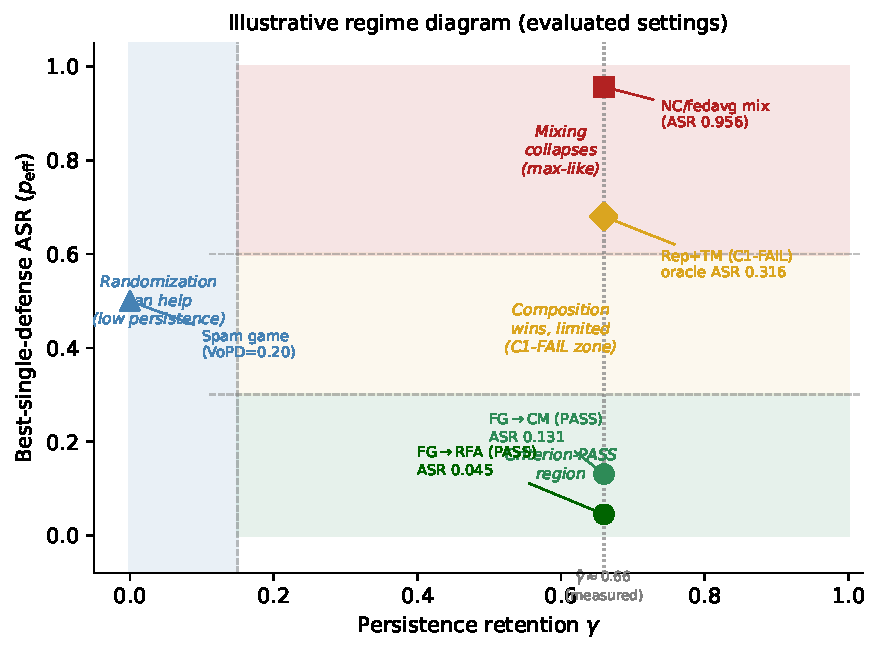
\includegraphics[width=0.62\linewidth]{figures/phase_boundary.pdf}
\caption{\textbf{The evaluated settings, plotted. No regimes, and one line, which is a measurement.} X-axis: persistence $\gamma$. Y-axis: best single-defense ASR ($p_\text{eff}$). Each marker is a setting we ran and carries its own measured value; the dotted line is the measured FL persistence $\hat\gamma \approx 0.66$. \textbf{An earlier version shaded four regime bands and drew threshold guides at $\gamma{=}0.15$, $p_\text{eff}{=}0.3$ and $p_\text{eff}{=}0.6$; none of those numbers was measured, so all six are gone.} Five points cannot locate a boundary, and nothing here is evidence of a phase transition in $(\gamma, p_\text{eff})$ space.}
\label{fig:regime}
\end{figure}

\noindent Figure~\ref{fig:regime} places the evaluated settings in the $(\gamma, p_{\mathrm{eff}})$ plane. At the persistence we measure ($\hat\gamma \approx 0.66$) the one temporal mix we ran reaches ASR $0.956$, which is the reason the paper composes rather than switches; the figure records those points and draws no boundary between them.

\paragraph{FL configuration.} $N{=}10$ clients, $K{=}5$ per round, 50 rounds, SGD with momentum 0.9, learning rate 0.01, local epochs 3, batch size 32, Dirichlet $\alpha{=}0.5$ (non-IID). Scale experiments: $N{=}100$, $K{=}10$, $f{=}0.05$, ResNet18 with GroupNorm.

\paragraph{Attacks.} Model-scaling: scale factor 10, 50\% poison fraction, target class 0. Pixel backdoor: $5{\times}5$ bottom-right trigger, target class 0. DBA: 4 sub-triggers at image corners, $f{=}0.4$/$0.6$. Joint-constraint: $\epsilon \in \{0.5, 1.0, 2.0, 4.0\}$, disjoint coordinate blocks per adversary, single-step $\epsilon$-ball projection per round.

\paragraph{Defenses.} NormClip $\tau{=}5.0$, i.e.\ $u_i \mapsto u_i\min(1, \tau/\|u_i\|_2)$ over the whole flattened update; TrimmedMean $\beta{=}0.2$ (trim 20\% each tail); RFA: unweighted Weiszfeld, 50 iterations, tolerance $10^{-6}$, initialised at the mean; FoolsGold: $w_i \propto \log((1-s_i)/(s_i+\epsilon)+\epsilon)$ with $s_i$ the client's maximum absolute pairwise cosine similarity normalised by the round maximum, $\epsilon{=}10^{-5}$, then shifted by $-\min_i$ and normalised, so the least-trusted client of each round receives weight exactly $0$ (empirically 2 of 5 clients per round).

\paragraph{Reputation.} Despite the name this defense is \emph{memoryless}, it keeps no cumulative per-client state and is recomputed from scratch each round from that round's $K$ participants. Consensus is the coordinate-wise median $m$ of the $K$ updates; scores are $\ell_2$ distances $d_i = \|u_i - m\|_2$; the bandwidth is adaptive, $\sigma = \mathrm{median}_i(d_i)$ (clamped $\geq 10^{-6}$); weights are $w_i = \exp(-d_i/\sigma)$, normalised to sum to 1. No clipping, no initialisation. Its discriminative property is therefore \emph{consensus distance}, not similarity spread, which is why Proposition~\ref{prop:invariance}(c) predicts that $\cdot \to$ Reputation compositions fail C2. Weights are strictly positive, so Reputation never produces the zero vectors of Lemma~\ref{lem:annihilation}.

\paragraph{Adversary count per round.} Adversaries are the fixed client identities $\{0,\dots,fN-1\}$; each round samples $K$ participants uniformly without replacement from all $N$, with no stratification. For $N{=}10$, $f{=}0.2$, $K{=}5$ the per-round adversary count is hypergeometric: $P(n_a{=}0) = P(n_a{=}2) = 56/252 = 0.222$, $P(n_a{=}1) = 140/252 = 0.556$; measured over 100 rounds we observe $0.19/0.54/0.27$. Two consequences, both matching the data. CoordMedian's count majority $n_a < K/2 = 2.5$ holds for every attainable $n_a \in \{0,1,2\}$, i.e.\ in \emph{100\%} of rounds. TrimmedMean's budget is $\lfloor\beta K\rfloor = \lfloor 1.0 \rfloor = 1$, so it is exceeded whenever $n_a{=}2$: 22.2\% of rounds, ${\approx}11$ of 50. This is why FG$\to$TrimmedMean fails ($0.508$) while FG$\to$CoordMedian succeeds ($0.107$) under an otherwise identical upstream transform. We retain the pre-registered C3-FAIL label for FG$\to$TM; the count-budget violation is an additional mechanism, not a relabelling.

\paragraph{Theorem quantities.} FoolsGold weight ratio across 5 seeds $\times$ 20 rounds ($N{=}10$, $f{=}0.2$, model-scaling): max $\rho = 2.1$, giving extremeness ratio $S/\rho \geq 4.8$ with $S{=}10$ (regime A). Reputation, same protocol (5 seeds $\times$ 20 rounds, 81 rounds containing both adversarial and benign clients): $\rho$ mean $1.44{\times}10^{5}$, max $2.84{\times}10^{6}$, p95 $6.1{\times}10^{5}$; mean adversarial weight $4.83{\times}10^{-4}$ against mean benign weight $0.278$, and $w_a < 10^{-3}$ in 85\% of rounds. Reputation therefore fails the ordering condition by ${\sim}5$ orders of magnitude and suppresses via regime B instead. RFA, measured on the transformed points $u'_i = w_i u_i$ that RFA actually receives (25 adversary-present rounds over 3 seeds): FG zeroes every adversary in 32\% of rounds, where Lemma~\ref{lem:annihilation} applies and the measured contraction $1-\Lambda_a$ is $0.29$ on average (range $0.001$--$0.52$). In the other 68\% ($w_a > 0$) the separation condition of Theorem~\ref{thm:bounded_reweight}(2) is satisfied in \emph{every} round, with margin $\Delta'_{\mathrm{sep}}/2(R'_B{+}\delta') \geq 2.8$ (mean $3.2$) and $\delta'/R'_B$ mean $0.19$, max $0.72$. The two cases are exhaustive, so the analysis covers all measured rounds. Proposition~\ref{prop:invariance}(a) verified in the shipped implementation: FoolsGold's weight vector changes by at most $3\times 10^{-8}$ (float32 rounding) under NormClip across 1000 synthetic trials and live rounds in which 1--2 of 5 clients were genuinely clipped (raw norms up to $24.5$ against $\tau{=}5$). Exactly 2 of the 5 clients per round receive zero FoolsGold weight. \textbf{Corollary~\ref{cor:aggregate_mass} in full:} with $D_b := R'_B+\delta'$ bounding every benign residual and $D_a := \Delta'_{\mathrm{sep}}-R'_B-\delta' = (2m-1)D_b$ lower-bounding every adversarial one, the Weiszfeld coefficients satisfy $\sum_j 1/d_j \geq n_b/D_b$ and $1/d_a \leq 1/D_a$, so $\Lambda_a \leq (n_a/D_a)/(n_b/D_b + n_a/D_a) = n_a/(n_b(2m-1)+n_a)$. At $m\to1$ this is $n_a/(n_b+n_a)$, i.e.\ $40\%$ for $n_a{=}2$, $n_b{=}3$; at the measured $m \geq 2.82$ it is $\leq 12.6\%$, and at the all-round mean $m = 3.24$, $\leq 10.8\%$.

\paragraph{Pre-registration provenance.} We distinguish the tiers explicitly. The 18-pair development set is where the criterion was \emph{developed}; its predictions were not committed in advance and we report it as fit. The 24-pair held-out set was pre-registered in \texttt{pre\_registration\_wave2.md} and committed before those experiments ran; it contains no predicted-PASS pair, so it bears only on specificity. The out-of-sample PASS predictions (DBA transfer, $N{=}100$/ResNet18 scale transfer, composition dominance) were pre-registered separately in \texttt{pre\_registration\_oos\_pass.md}, also committed in advance. The 10 three-way predictions were pre-registered in \texttt{pre\_registration\_three\_way.md}. Two held-out LOW calls, hedged as speculative at pre-registration time, failed; we score them as misses rather than dropping them. The prospective suite of \S\ref{sec:prospective} was pre-registered in \texttt{pre\_registration\_prospective.md} at commit \texttt{262cf35}, which precedes the first write to \texttt{results/prospective\_suite/}; single-defense baselines for the three new defenses were measured \emph{before} the freeze, because C1 and C0 take them as inputs (FLTrust $0.048$, Krum $0.583$, Multi-Krum $0.783$ max-committed; FedAvg $0.667$ scaling / $0.768$ pixel, clearing the sanity gate). The predicted labels in that file are reproduced verbatim in the \texttt{PAIRS} list of \texttt{run\_prospective\_suite.py} and the confusion matrix is recomputed from per-seed ASR in \texttt{results/prospective\_suite/summary.json}, not transcribed.

\paragraph{Freeze commits and run tallies for the interventional suites.} Every design, grid and threshold below was git-committed before the corresponding results directory existed, and each hash is verifiable in the repository history. \emph{Dose--response ladder} (\S\ref{sec:dose_response}): \texttt{pre\_registration\_dose\_response.md} at commit \texttt{e711a95}, before \texttt{results/dose\_response/}; $80$ runs. \emph{Metric-swap mirrors} (\S\ref{sec:metric_swap}): $8$ frozen labels at commit \texttt{356897b}. \emph{Prospective suite} (\S\ref{sec:prospective}): commit \texttt{262cf35}, as above. \emph{Targeted intervention, Modes S and A} (\S\ref{sec:targeted}, \S\ref{sec:targeted_rest}): design and thresholds at commit \texttt{5130cec} before \texttt{results/targeted\_dose/} existed; $97$ runs plus $25$ identity runs verified bit-identical per seed (largest deviation $0.00\mathrm{e}{+}0$); the adversarial coefficient share was verified with no ASR involved, before any run. \emph{Rank-discordant replication} (\S\ref{sec:targeted}): \texttt{pre\_registration\_dose\_replication.md} at commit \texttt{06d9bce} before \texttt{results/dose\_replication/} existed; $15$ new runs, identity rung imported bit-identical from the ladder and verified by \texttt{--harness-check}. \emph{Second dataset and architecture} (\S\ref{sec:targeted}): \texttt{pre\_registration\_dose\_femnist.md} at commit \texttt{478b555} before \texttt{results/dose\_femnist/} existed; $12$ new runs, with $\kappa{=}0$ run in-suite because no EMNIST-byclass ladder exists to import from. \emph{Score-only control} (\S\ref{sec:targeted}, Appendix~\ref{app:score_only}): \texttt{pre\_registration\_score\_only.md} at commit \texttt{35788d9} before \texttt{results/score\_only/} existed; $15$ new runs, identity rung imported bit-identical and verified by \texttt{--harness-check}, and the \texttt{cos\_krum} corollary checked at one seed as pre-registered.

\end{document}
